\section{Invariant mass fits}
\label{sec:rkst_fits}

The signal yields are obtained using a simultaneous unbinned maximum likelihood fit
to the 4-body invariant mass, $m(K\pi\ell\ell)$, of the rare, normalisation and control samples.
The simultaneous fit allows to share parameters \eg those describing data-simulation differences.
The yields of the rare channels are parameterised as a function of the corresponding \jpsi yields as
%
\begin{equation}
N_{\ell\ell}(r_{\ell\ell}, N_{\jpsi}) = N_{\jpsi} \cdot \varepsilon^{\rm rel} \cdot r_{\ell\ell},
\end{equation}
%
where $\varepsilon^{\rm rel}$ is the relative efficiency between the rare and resonant channels
(given in Tab.~\ref{tab:RKst_RelEff}). Consequently, $r_{\ell\ell}$ corresponds to the efficiency corrected
ratio between the raw rare and resonant yields:
%
\begin{equation}
r_{\ell\ell} = \frac{N_{\ell\ell} / \varepsilon^{\ell\ell}}{N_{\jpsi} / \varepsilon^{\jpsi(\ell\ell)}}.
\end{equation}
%
The two ratios, $r_{ee}$ and $r_{\mu\mu}$, are then used to determine
the \RKst quantity, as described in Sec.~\ref{sec:RKst_result}.
The following subsections contain a description of the line shapes used to model
the signal and background components in each sample.
%The definition of these shapes follows the steps:
%\begin{itemize}
%\item fit simulated signal candidates
%\item fix some parameters in order to obtain shapes which depend on a limited set of parameters
%\item	
%\end{itemize}

\subsection{Muon channels}

For the rare and resonant $\mu\mu$ channels the fitted variable is the $m(K\pi \mu\mu)$ invariant mass coming
from a kinematic fit where all vertices are required to point to their mother particle.
In the resonant case it is beneficial to also constrain the dimuon mass to the known \jpsi mass;
in this case the invariant mass is referred to as $m(K\pi \mu\mu)_\jpsi$.
The effect of the kinematical constraint is to improve the mass resolution by roughly a factor of 2, which results
in a more stable fit. Furthermore, partially reconstructed background candidates are pushed away from
the \Bz peak towards low invariant mass values. %, which allows to use a wider mass window to better constrain the combinatorial background slope.
The mass spectrum is fitted in the range 5150 -- 5800~\mevcc~ with the lower limit
chosen to totally exclude the partially reconstructed background.
As it is not needed to model partially reconstructed backgrounds in the fit this also
eliminates the systematic uncertainties associated with the knowledge of their shape. 

\subsubsection{\BdToKstJPsmm PDF}

The signal PDF adopted to describe the reconstructed 4-body invariant mass of \BdToKstJPsmm candidates is the 
sum of a Double Crystal Ball~\cite{Skwarnicki:1986xj} (DCB) function with opposite-side tails and a Gaussian function with 
a common mean, $\mu$:
%
\begin{equation*}
\begin{array}{rl}
\mathcal{P}_{\rm sig}(m | \vec{\lambda}) = & 
f_{\rm CB1} \cdot \mathcal{P}_{\rm CB}(m | \mu, \sigma_1, \alpha_1, n_1) \, + \\
& f_{\rm CB2} \cdot \mathcal{P}_{\rm CB}(m | \mu, \sigma_2, \alpha_2, n_2) \, 
+ (1 - f_{\rm CB1} -f_{\rm CB2}) \cdot \mathcal{P}_{\rm Gauss}(m | \mu, \sigma_3) \, ,
\end{array}
\end{equation*}
where $f_{{\rm CB}i}$ is the relative fraction of candidates falling in the $i^{th}$ Crystal Ball function, $\sigma_i$ is the width, $\alpha_i$ and $n_i$ are the parameters controlling the power law tail of each CB, and $\sigma_3$ is the width of the Gaussian function.

As a first step, the parameters of the signal PDF are extracted by fitting the $\mcKpimm_{\jpsi}$ distribution 
of \BdToKstJPsmm simulated candidates; parameters are then fixed for the fit to the data.
Figure~\ref{fig:mumu_MC_fits_main} shows the fitted simulated distribution for the normalisation channel, while
fits or the rare channel in the three \qsq bins are reported in Appendix~\ref{app:RKMCfits}.
In order to account for possible discrepancies in the invariant mass distribution between data and simulation, the mass is allowed to shift, $\mu \rightarrow \mu +m'$, and the widths are allowed to scale, $\sigma_i \rightarrow c \cdot \sigma_i$, where 
the scale factor $c$ is common between the three $\sigma$s.
%
\begin{figure}[h!]
\centering 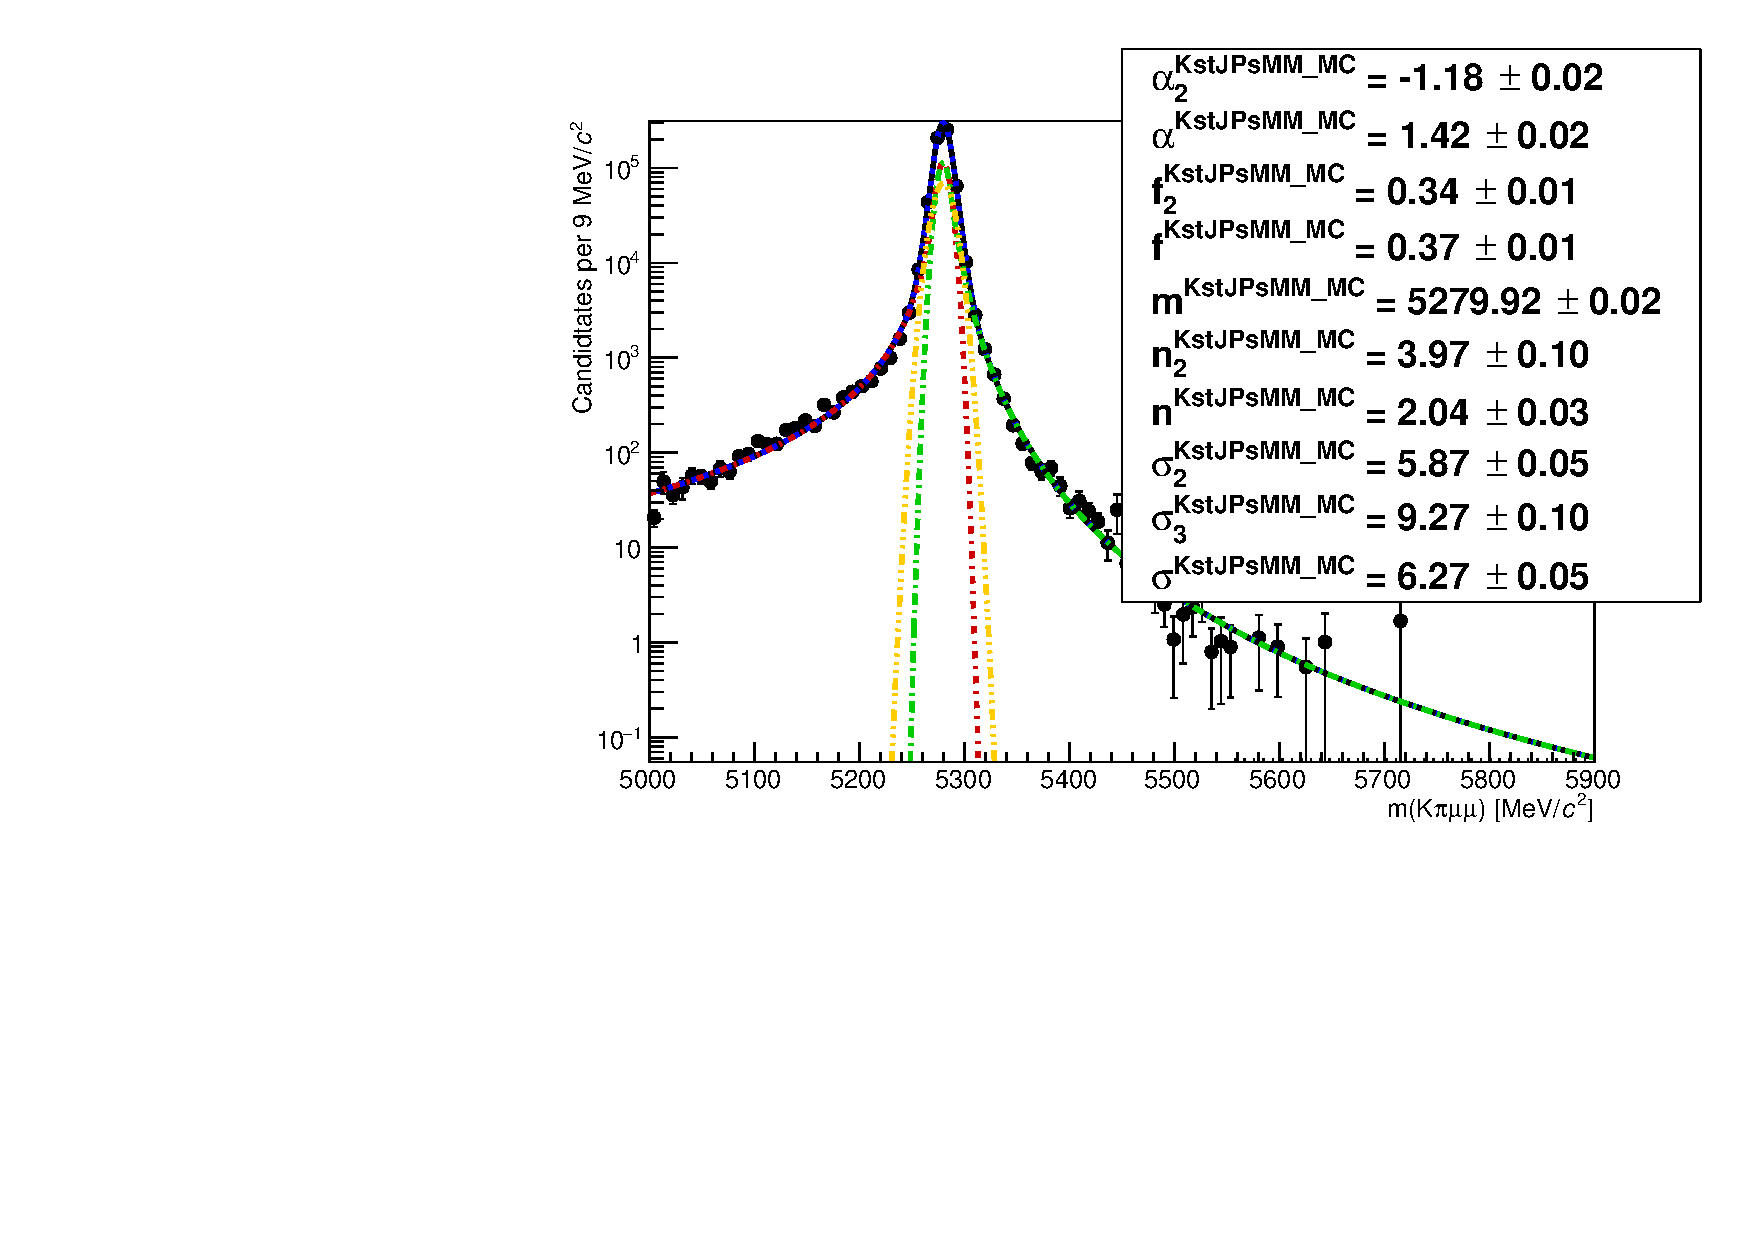
\includegraphics[width=0.7\textwidth]{RKst/figs/Fit/fit_MM/KstJPsMM_MC_log.pdf}
%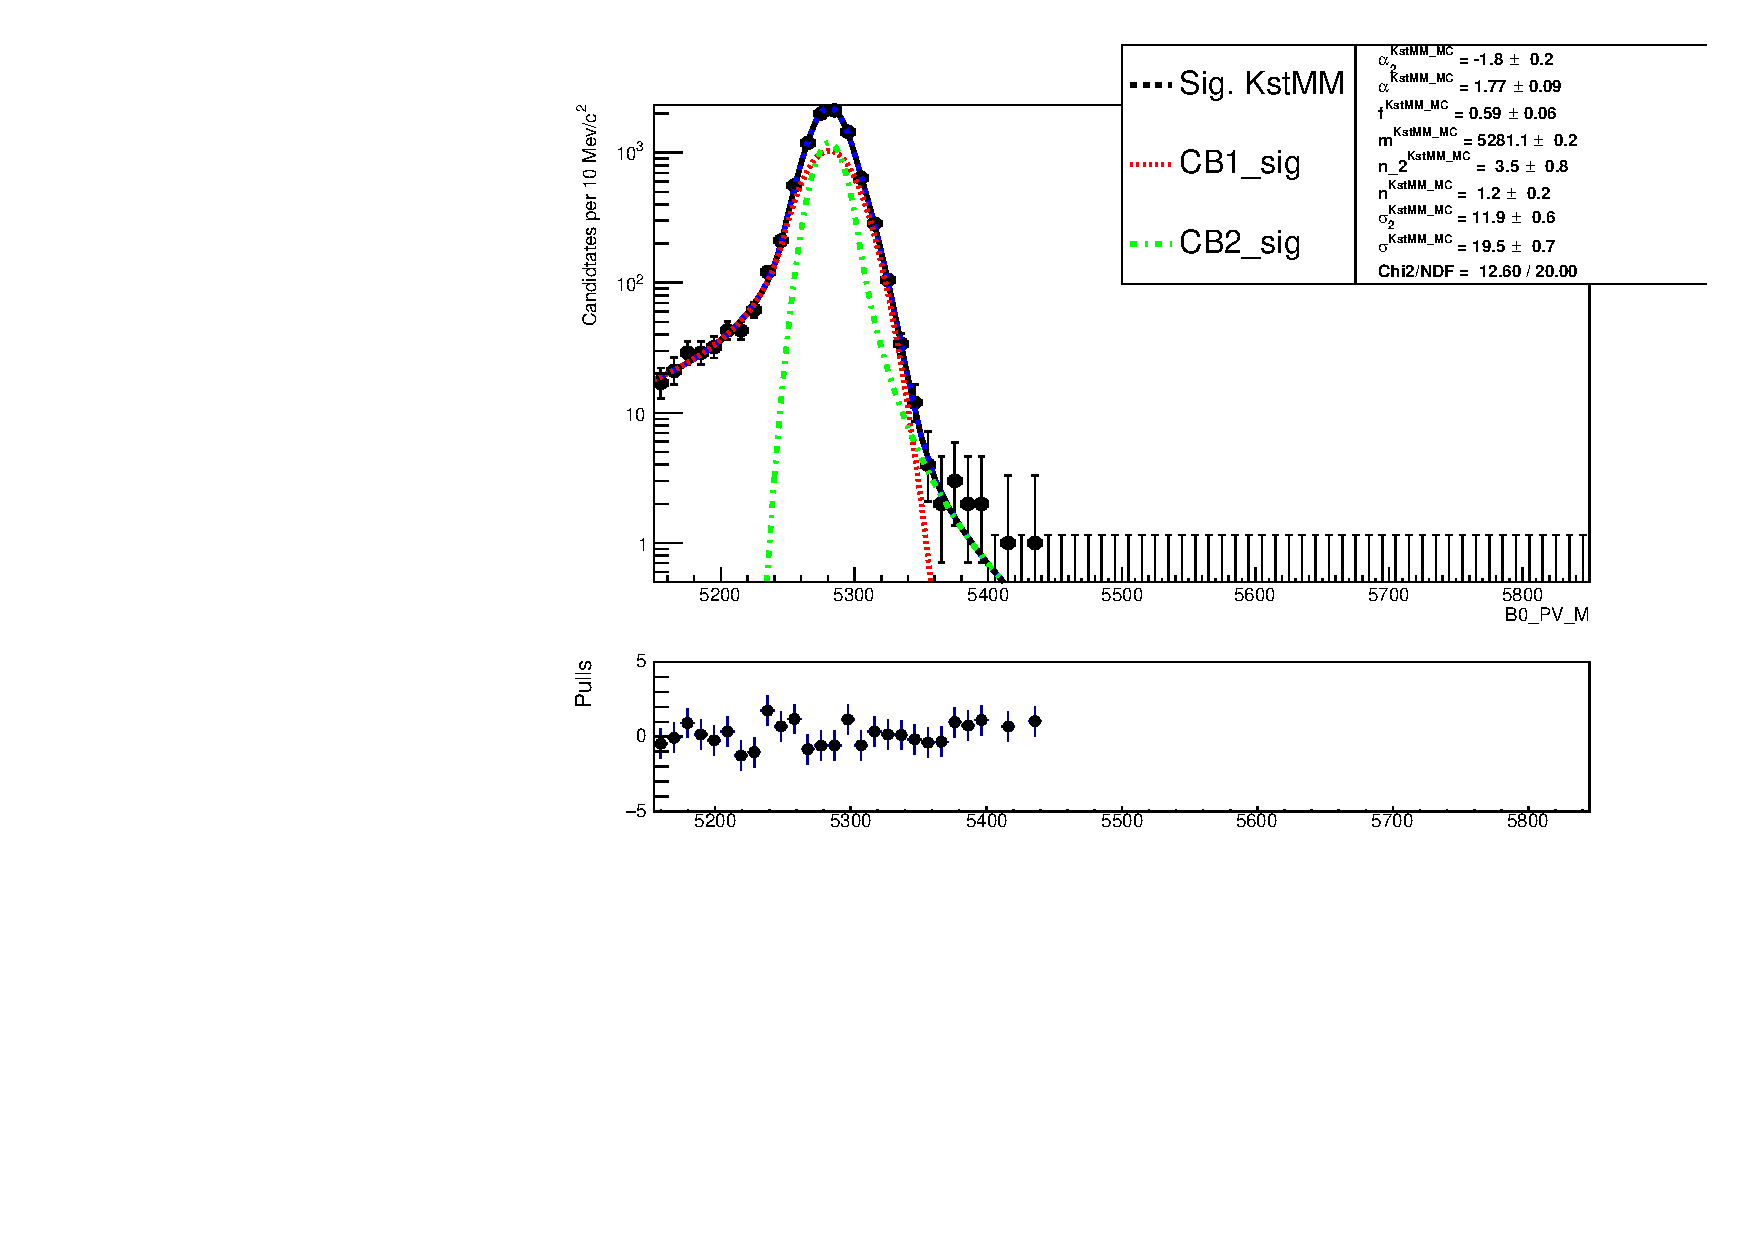
\includegraphics[width=0.48\textwidth]{figs/Fit/KstMM_MC_log_fitAndRes.pdf}
%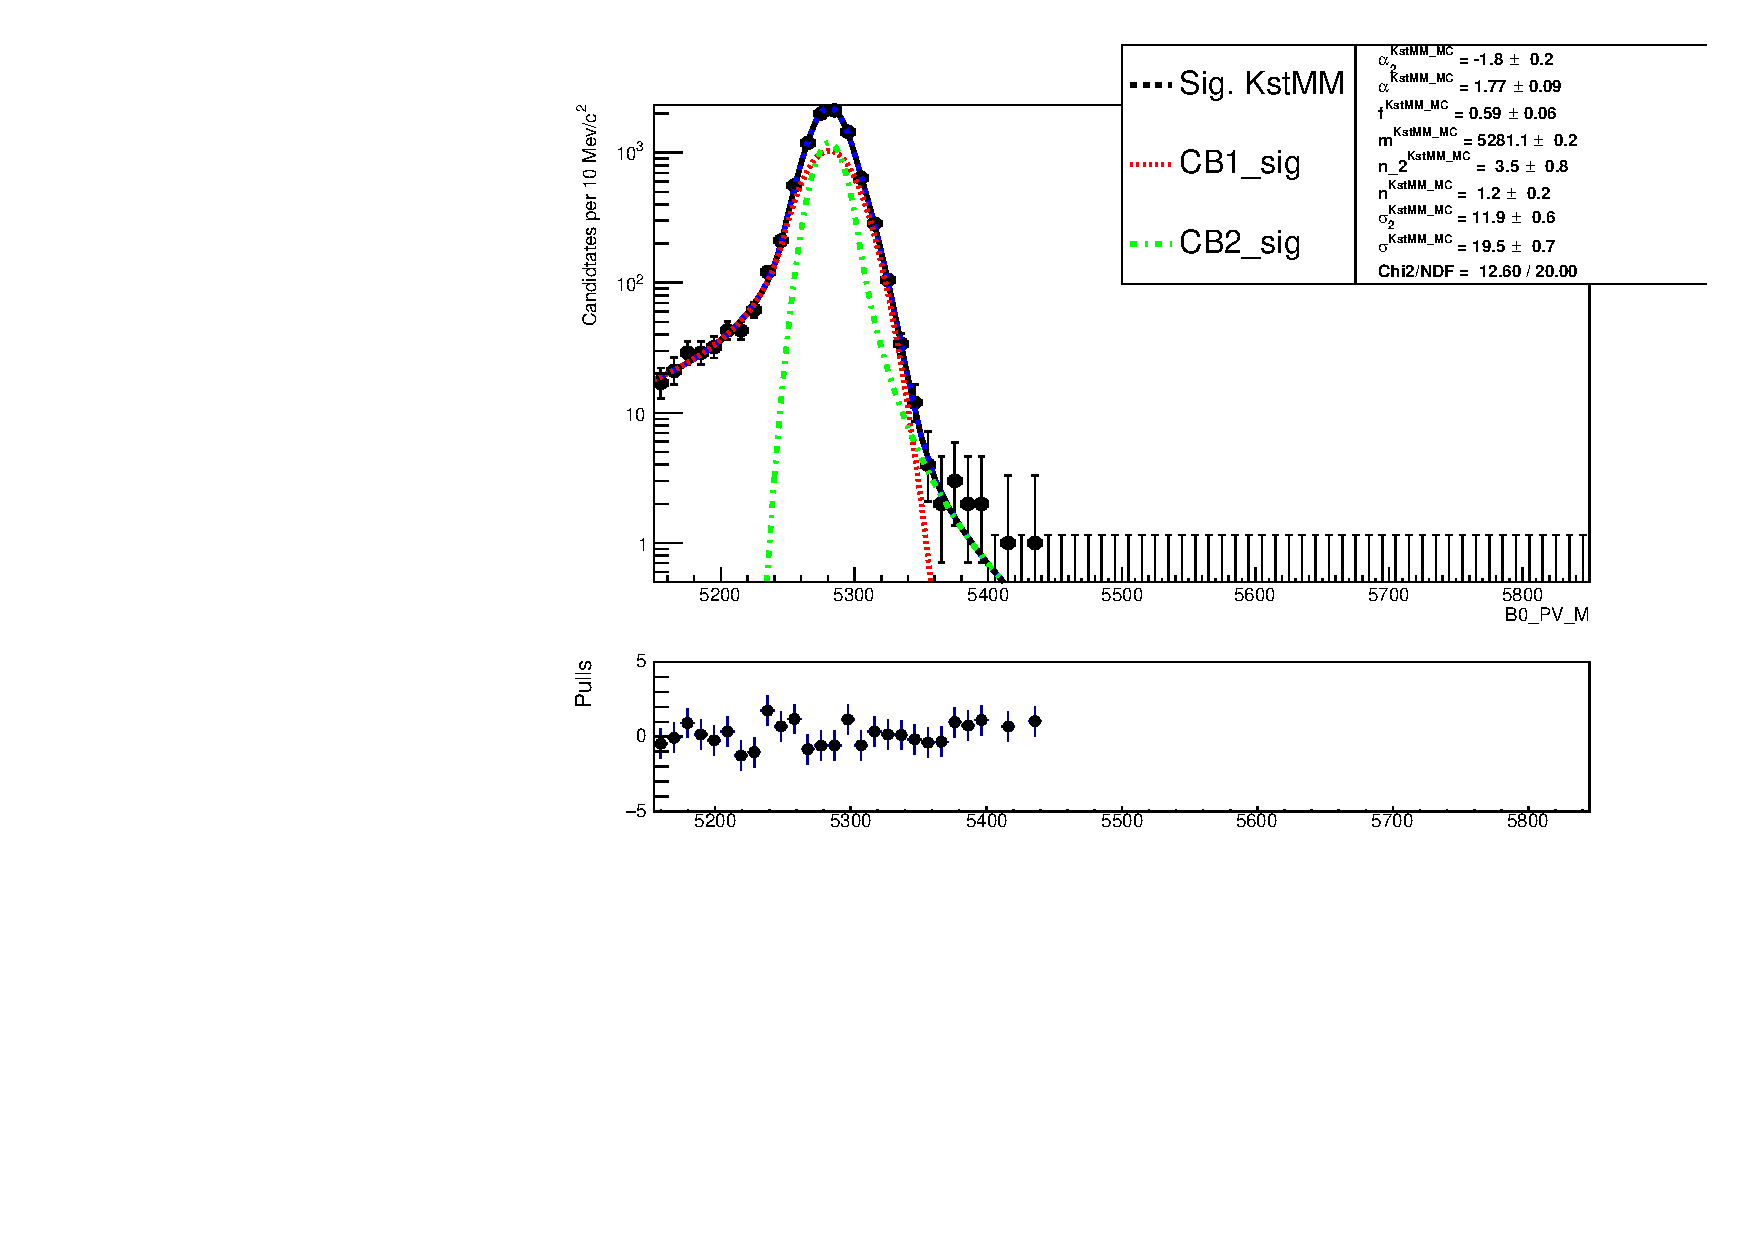
\includegraphics[width=0.48\textwidth]{figs/Fit/KstMM_MC_log_fitAndRes.pdf}
\caption{Fitted $m(K\pi \mu\mu)_{\jpsi}$ mass spectrum for $\Kstarz\jpsi$ simulated events. }
\label{fig:mumu_MC_fits_main}
\end{figure}
%
%The parameter $m'$ is common between the resonant and the rare samples.
%
%For the same reason the widths are allowed to scale, $\sigma_i \rightarrow c \cdot \sigma_i$, where 
%the scale factor $c$ is common between the three $\sigma$s.

In summary, the signal PDF for the $\jpsi(\mu\mu)$ channel fit on data is defined as
%
\begin{equation*}
\begin{array}{rl}
\mathcal{P}_{\rm \jpsi(\mu\mu)}(m | m', c) = &
f_{\rm CB1} \cdot \mathcal{P}_{\rm CB}(m | m', c) + 
f_{\rm CB2} \cdot \mathcal{P}_{\rm CB}(m | m', c) \,+ \\ 
& (1 - f_{\rm CB1} -f_{\rm CB2}) \cdot \mathcal{P}_{\rm Gauss}(m | m', c) \, .$$
\end{array}
\end{equation*}
%
where the only free parameters are the mass shift, $m'$ and the width scale factor, $c$.


The following backgrounds are considered:

\begin{itemize}

\item \textit{Combinatorial}: modelled with an exponential function;

\item \LbTopKJPsmm: described using fully reconstructed simulated events to which the full selection is applied;
%and weights for the $p\kaon$ Dalitz plot are applied; 
this distribution has a broad shape under the signal peak and is smoothed 
using the \verb!RooKeysPdf! class of the \roofit~\cite{Verkerke:2003ir} package;

\item \BsToKstJPsmm: described using the same PDF adopted for the signal, but a different central 
value, $\mu$, which is set at the \Bs nominal mass. The same shift $m'$  is used as for the signal.
%This component is considered only for the fit of the resonant mode, as it is negligible in the rare mode. 

\end{itemize}


\subsubsection{\BdToKstmm PDF}

%The PDF chosen to describe the \Bz invariant mass of \BdToKstmm candidates is a DCB function.
The signal PDF adopted to describe the reconstructed 4-body invariant mass of the rare \BdToKstmm candidates 
is a DCB function with opposite-side tails with a common mean, $\mu$.
The parameters of the PDF are fixed to values obtained by fitting simulated candidates, separately in each \qsq interval.
As for the charmonium channel, the mass is allowed to shift and the widths are allowed to scale with a common factor:
%
$$\mathcal{P}_{\rm \mm, \qsq}(m | m'_{\qsq}, c_{\qsq}) = 
f_{\rm core, \qsq} \cdot \mathcal{P}_{\rm CB}(m | m'_{\qsq}, c_{\qsq}) + 
(1 - f_{\rm core, \qsq}) \cdot \mathcal{P}_{\rm CB}(m | m'_{\qsq}, c_{\qsq}).$$
%
where $f_{\rm core, \qsq}$ is the relative fraction of candidates falling in the first Crystal Ball function, $m'_{\qsq}$ is the mass shift and $c_{\qsq}$ is the width scale.
The subscript ``$q^2$" indicates that independent parameters are used for each \qsq interval.
The background is described by an exponential function in all the three \qsq intervals.

\subsubsection{Summary}

In summary, the free parameters of the simultaneous fit to the $\jpsi(\mu\mu)$ and $\mu\mu$ candidates are the signal and background yields, the combinatorial background slopes, the mass shifts and the width scales.
Figure~\ref{fig:mumu_data_fits} shows the results of the fit to the rare and resonant
$\mu\mu$ candidates. Values of the fitted parameters are reported on the plots.
%
\begin{figure}[bh!]
\centering
%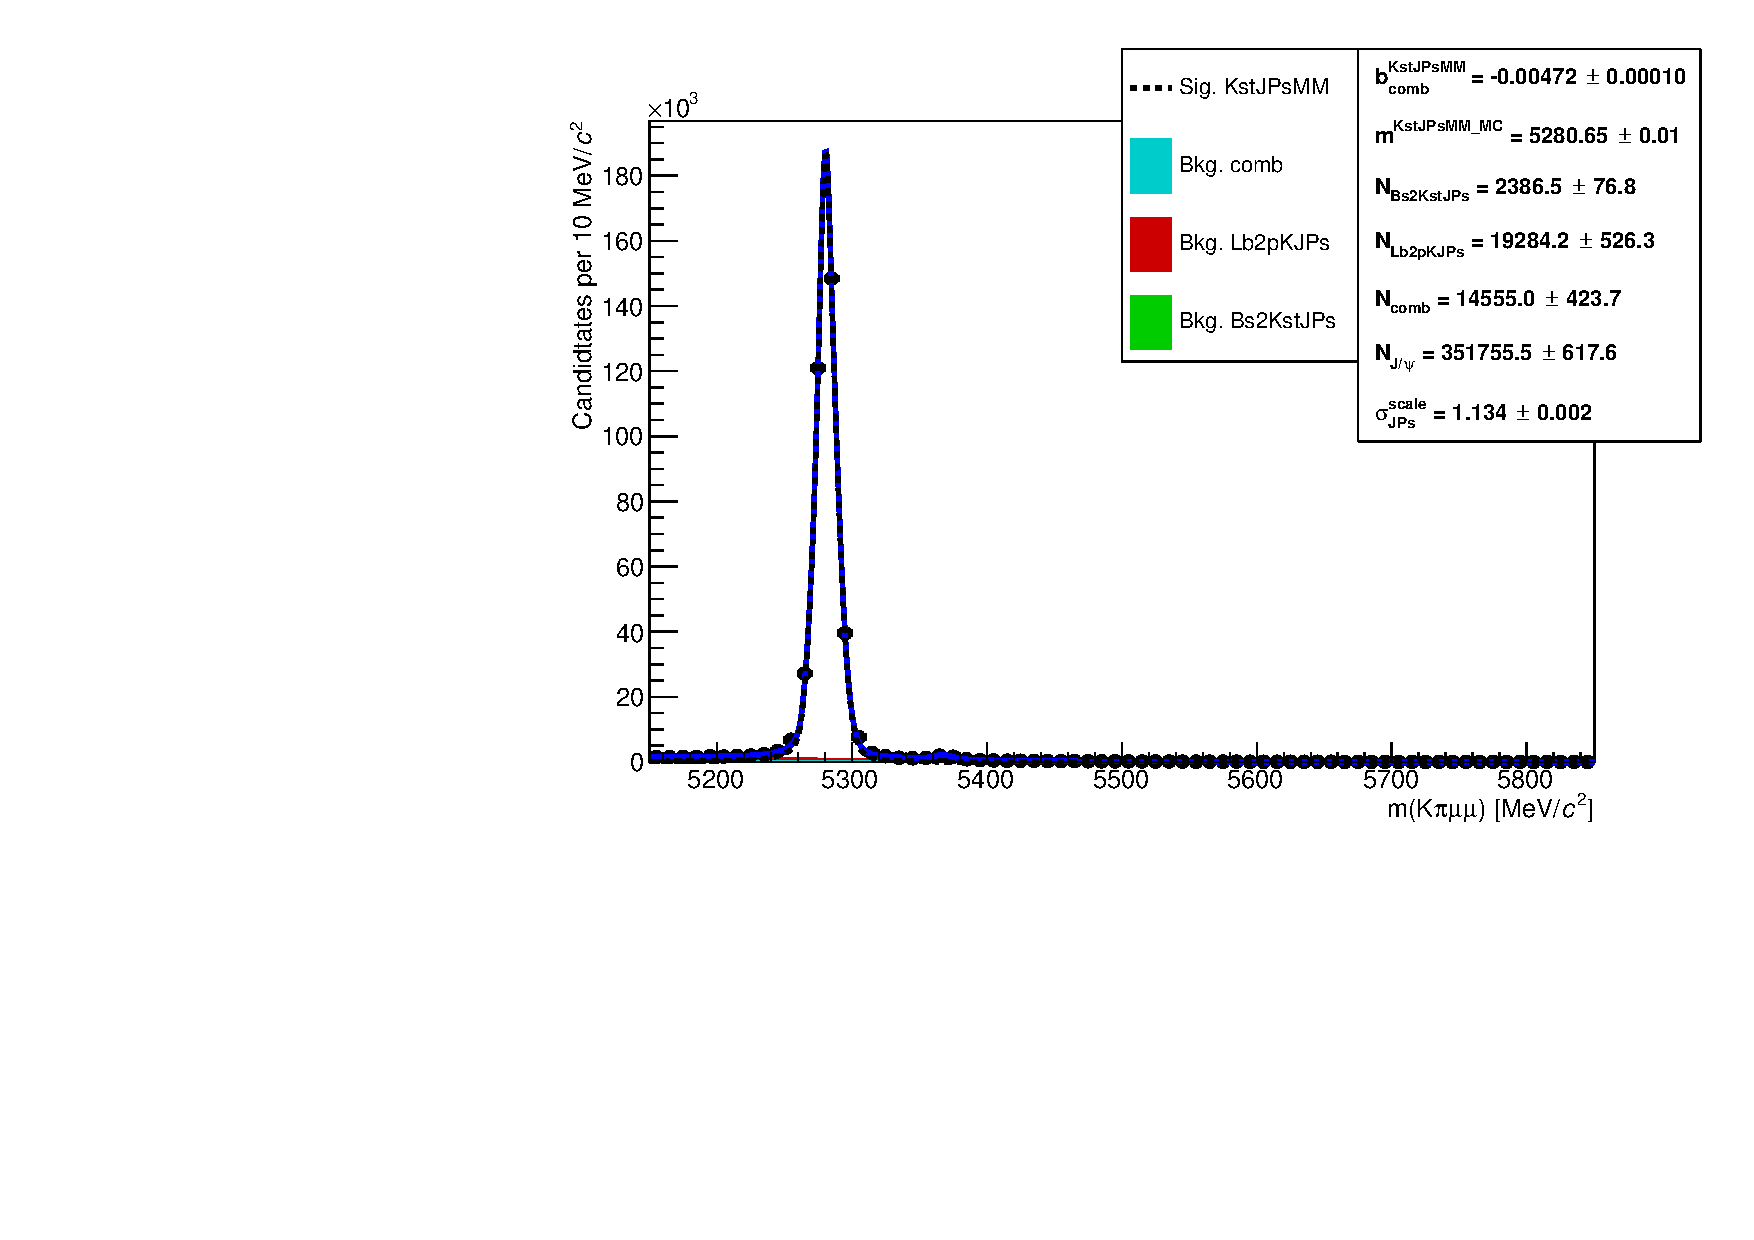
\includegraphics[width=0.49\textwidth]{RKst/figs/Fit/fit_MM/KstJPsMM.pdf}
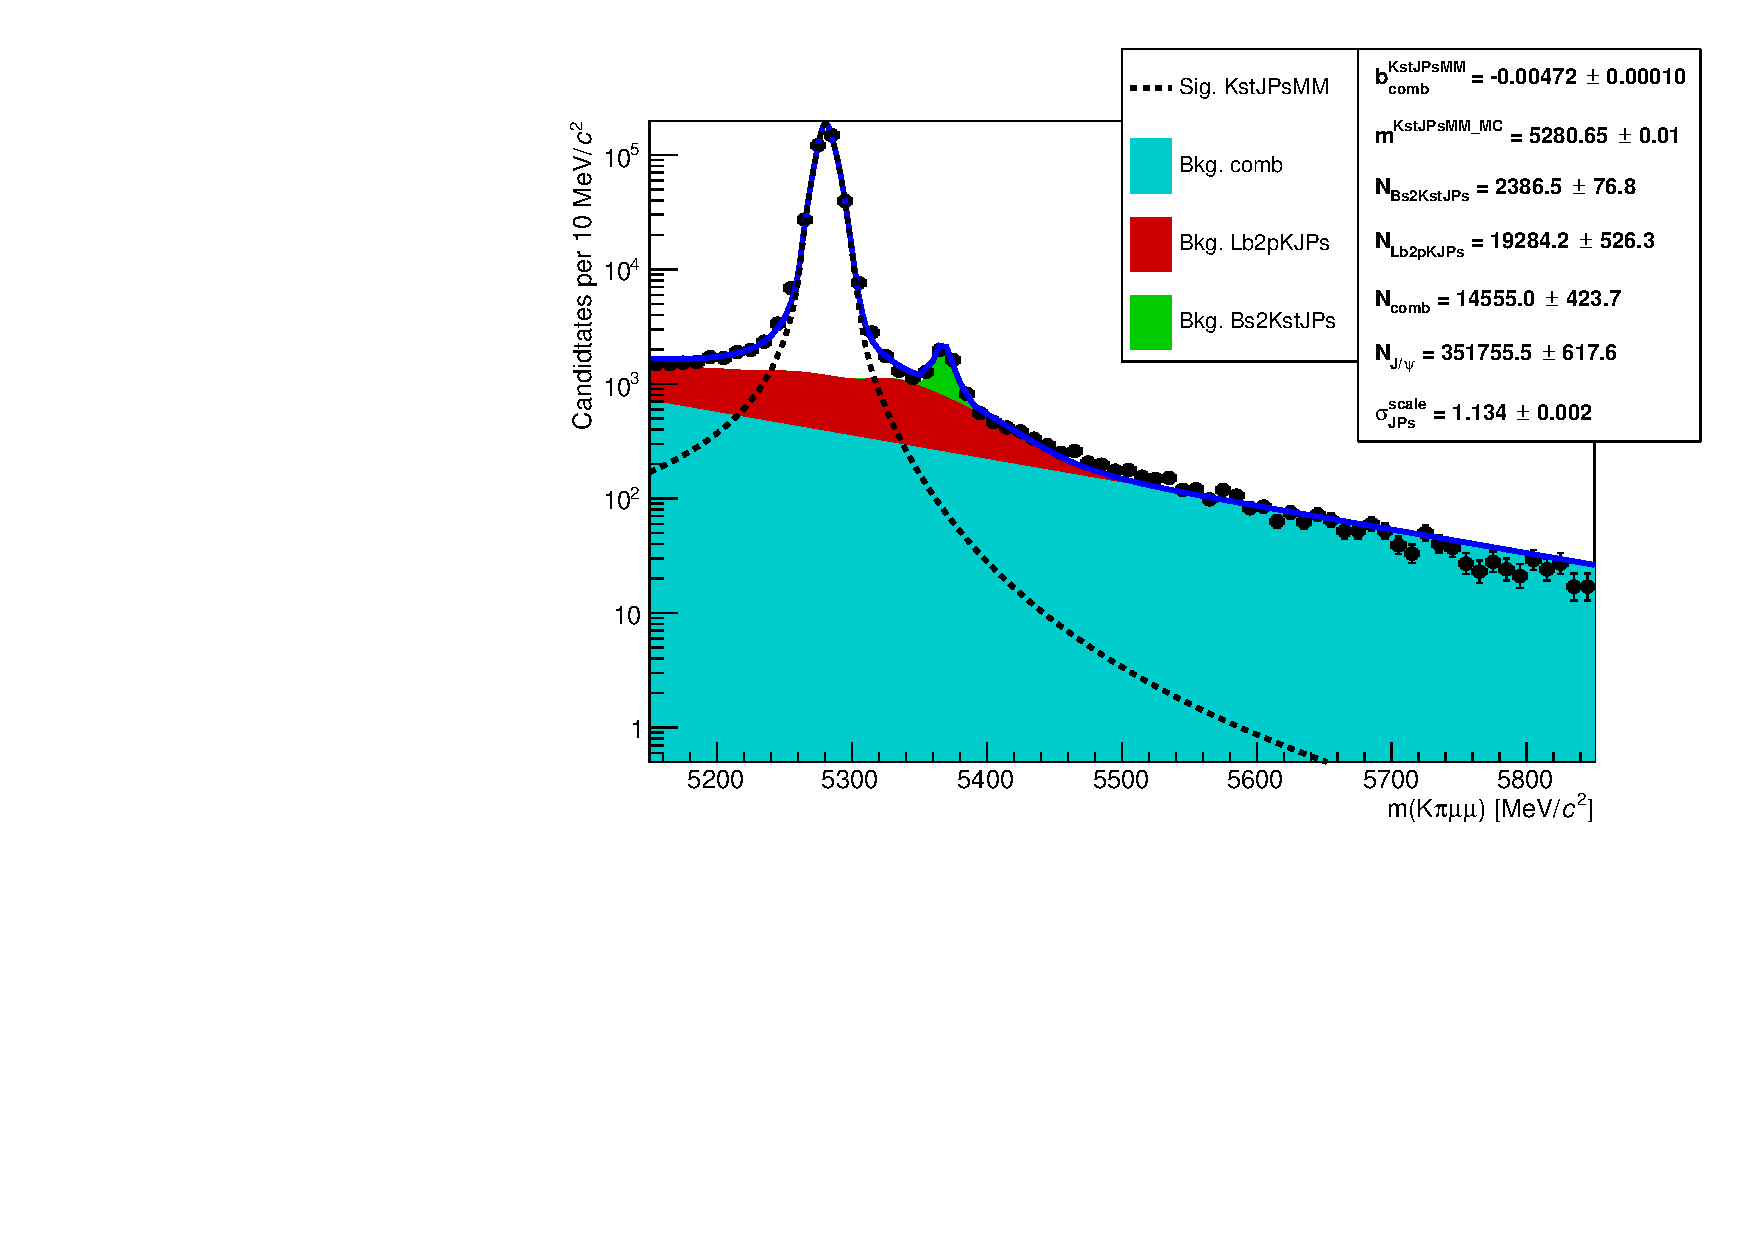
\includegraphics[width=0.7\textwidth]{RKst/figs/Fit/fit_MM/KstJPsMM_log.pdf}
%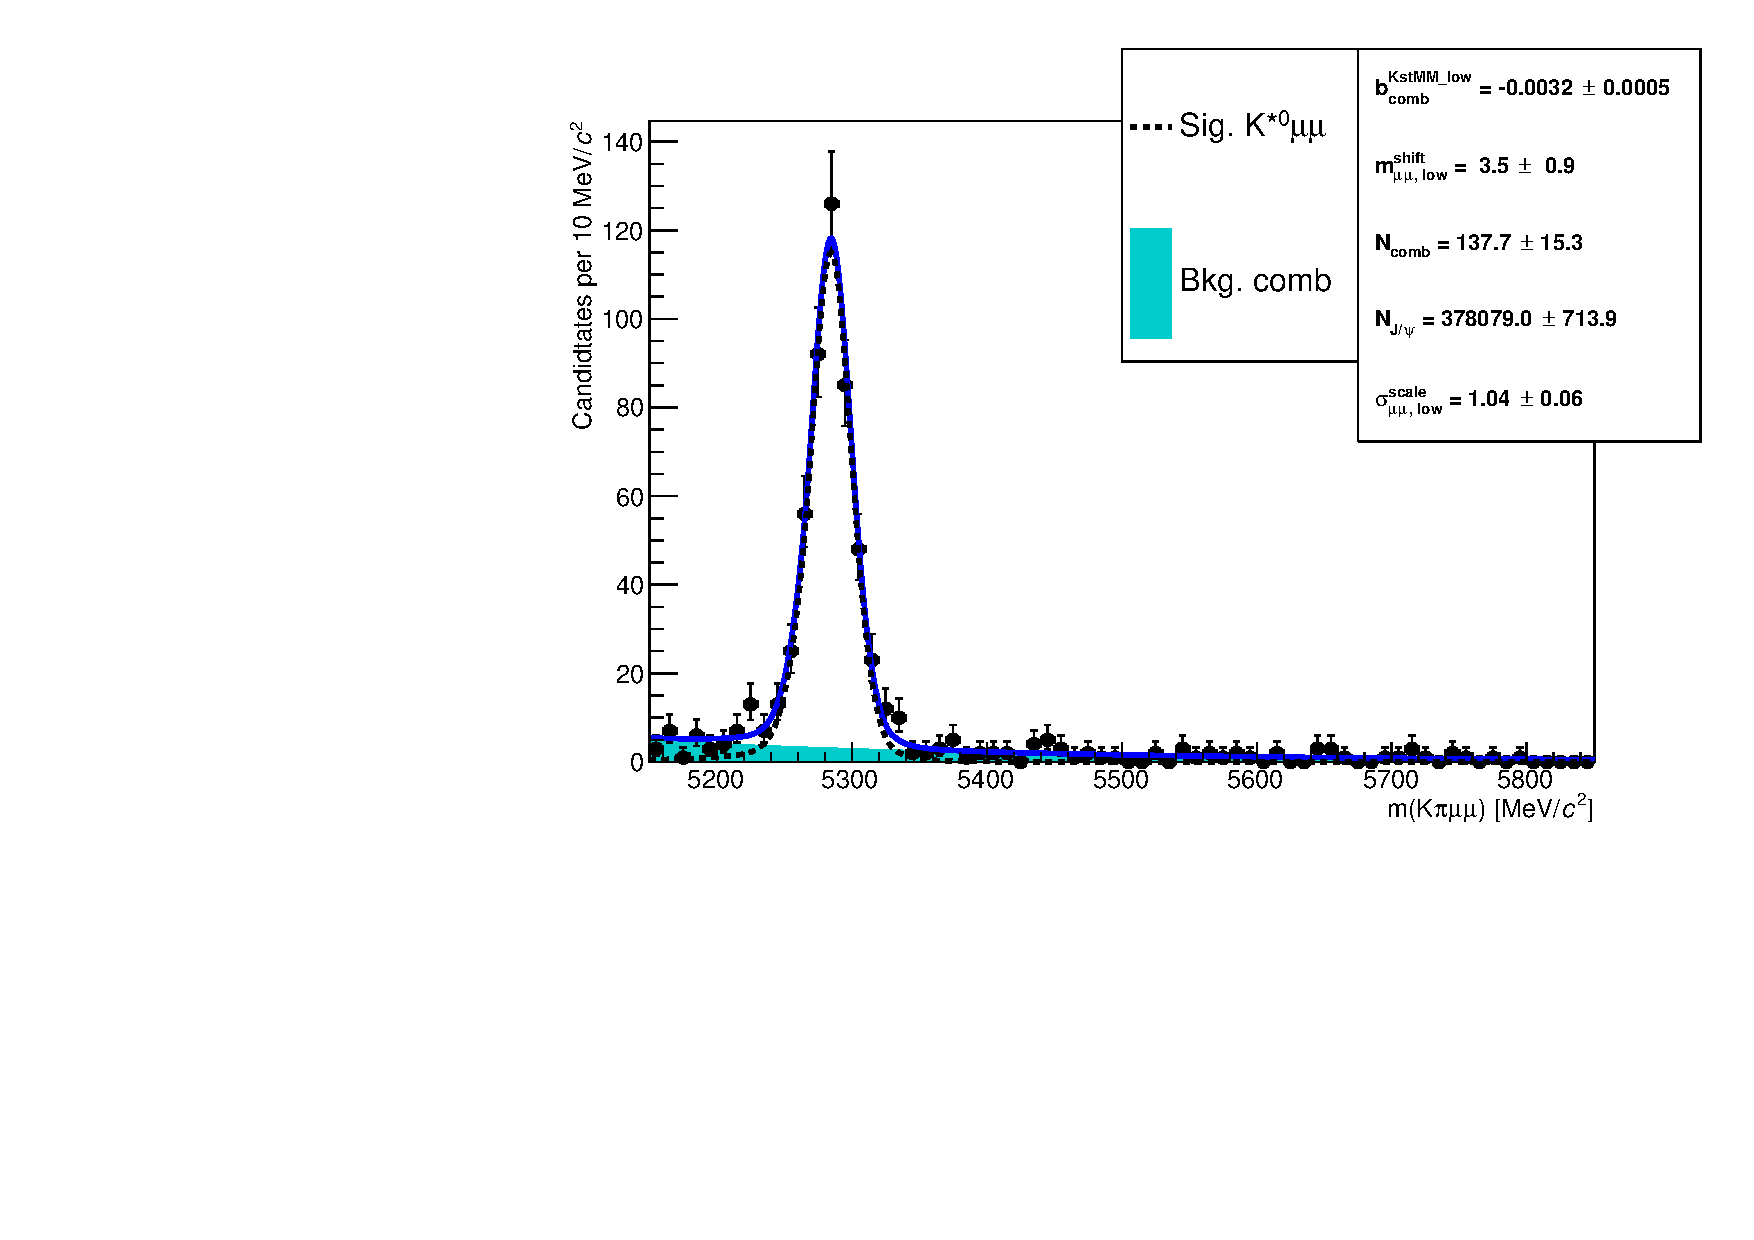
\includegraphics[width=0.55\textwidth]{RKst/figs/Fit/fit_MM/KstMM_low.pdf}
%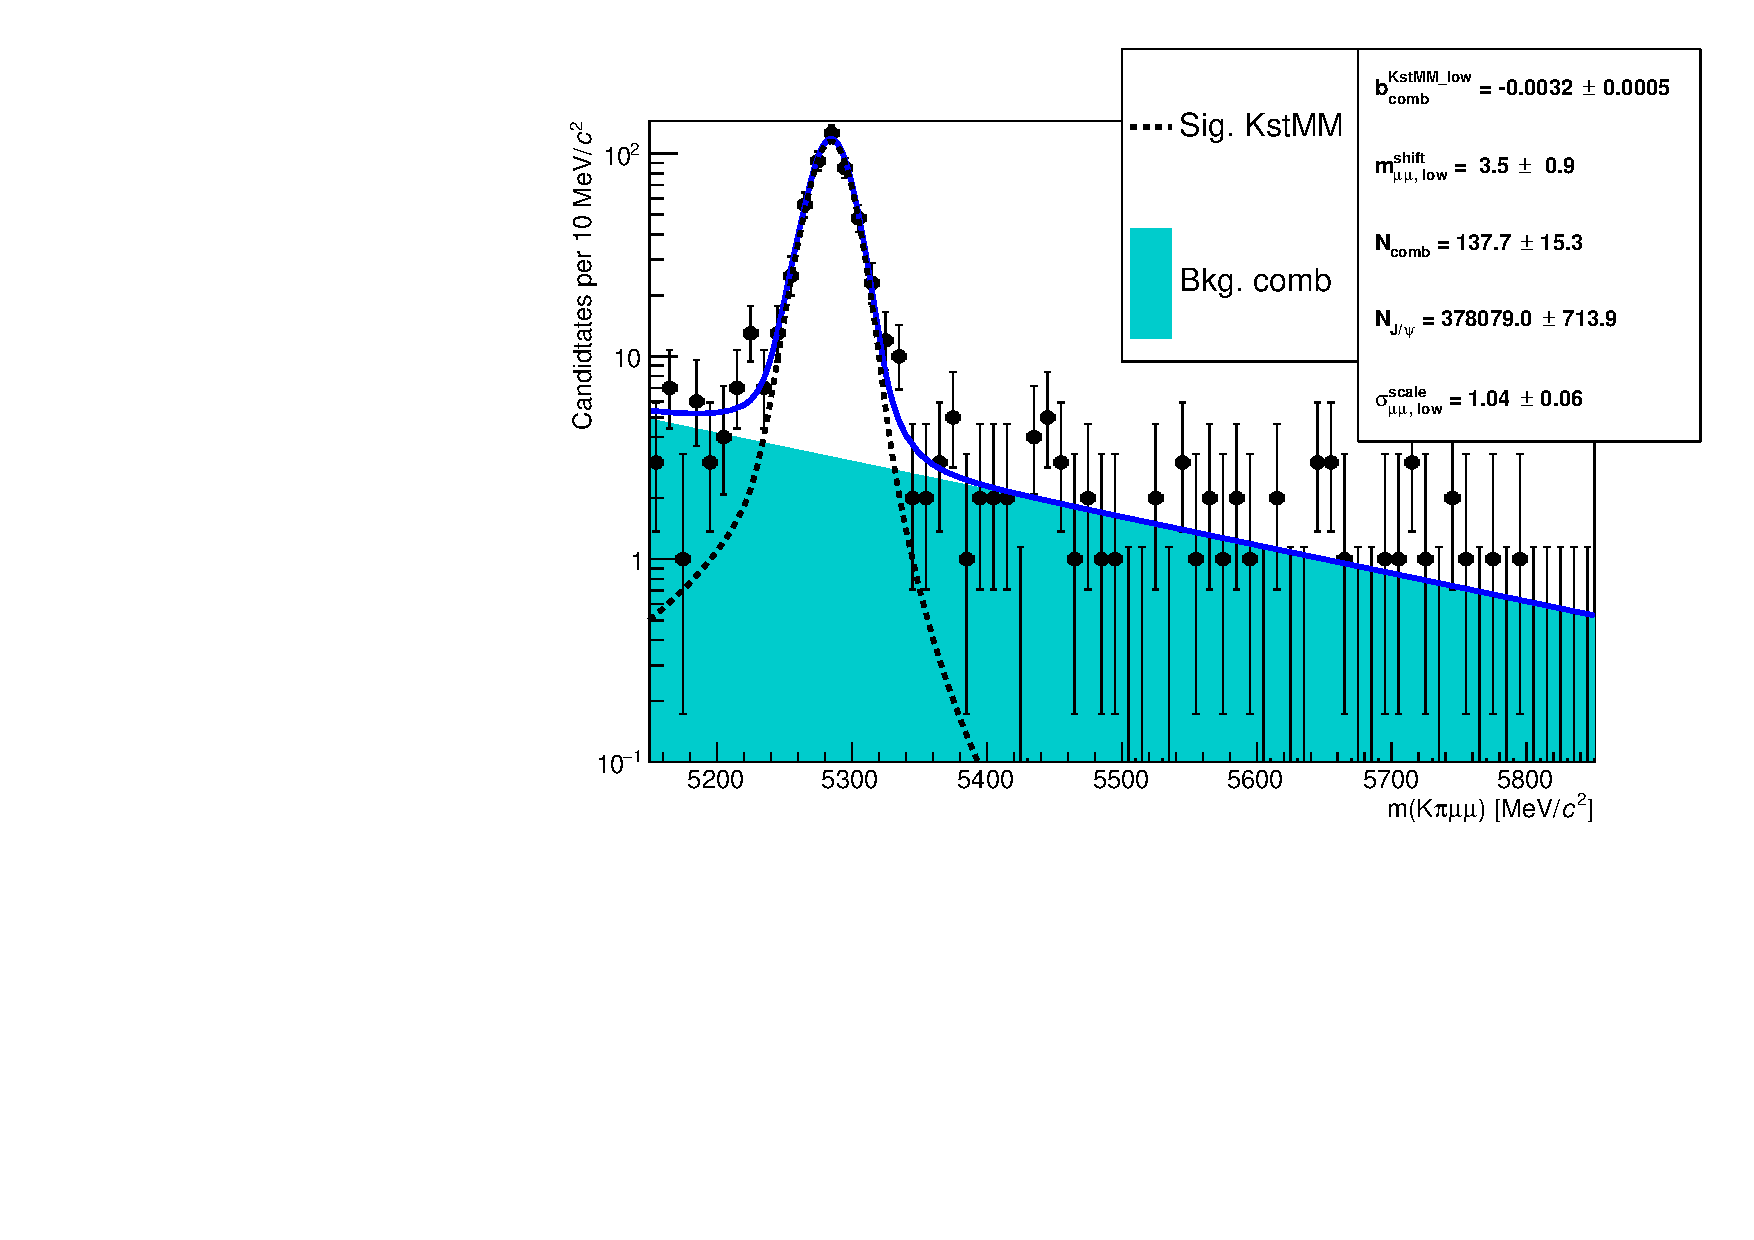
\includegraphics[width=0.49\textwidth]{RKst/figs/Fit/fit_MM/KstMM_low_log.pdf}
%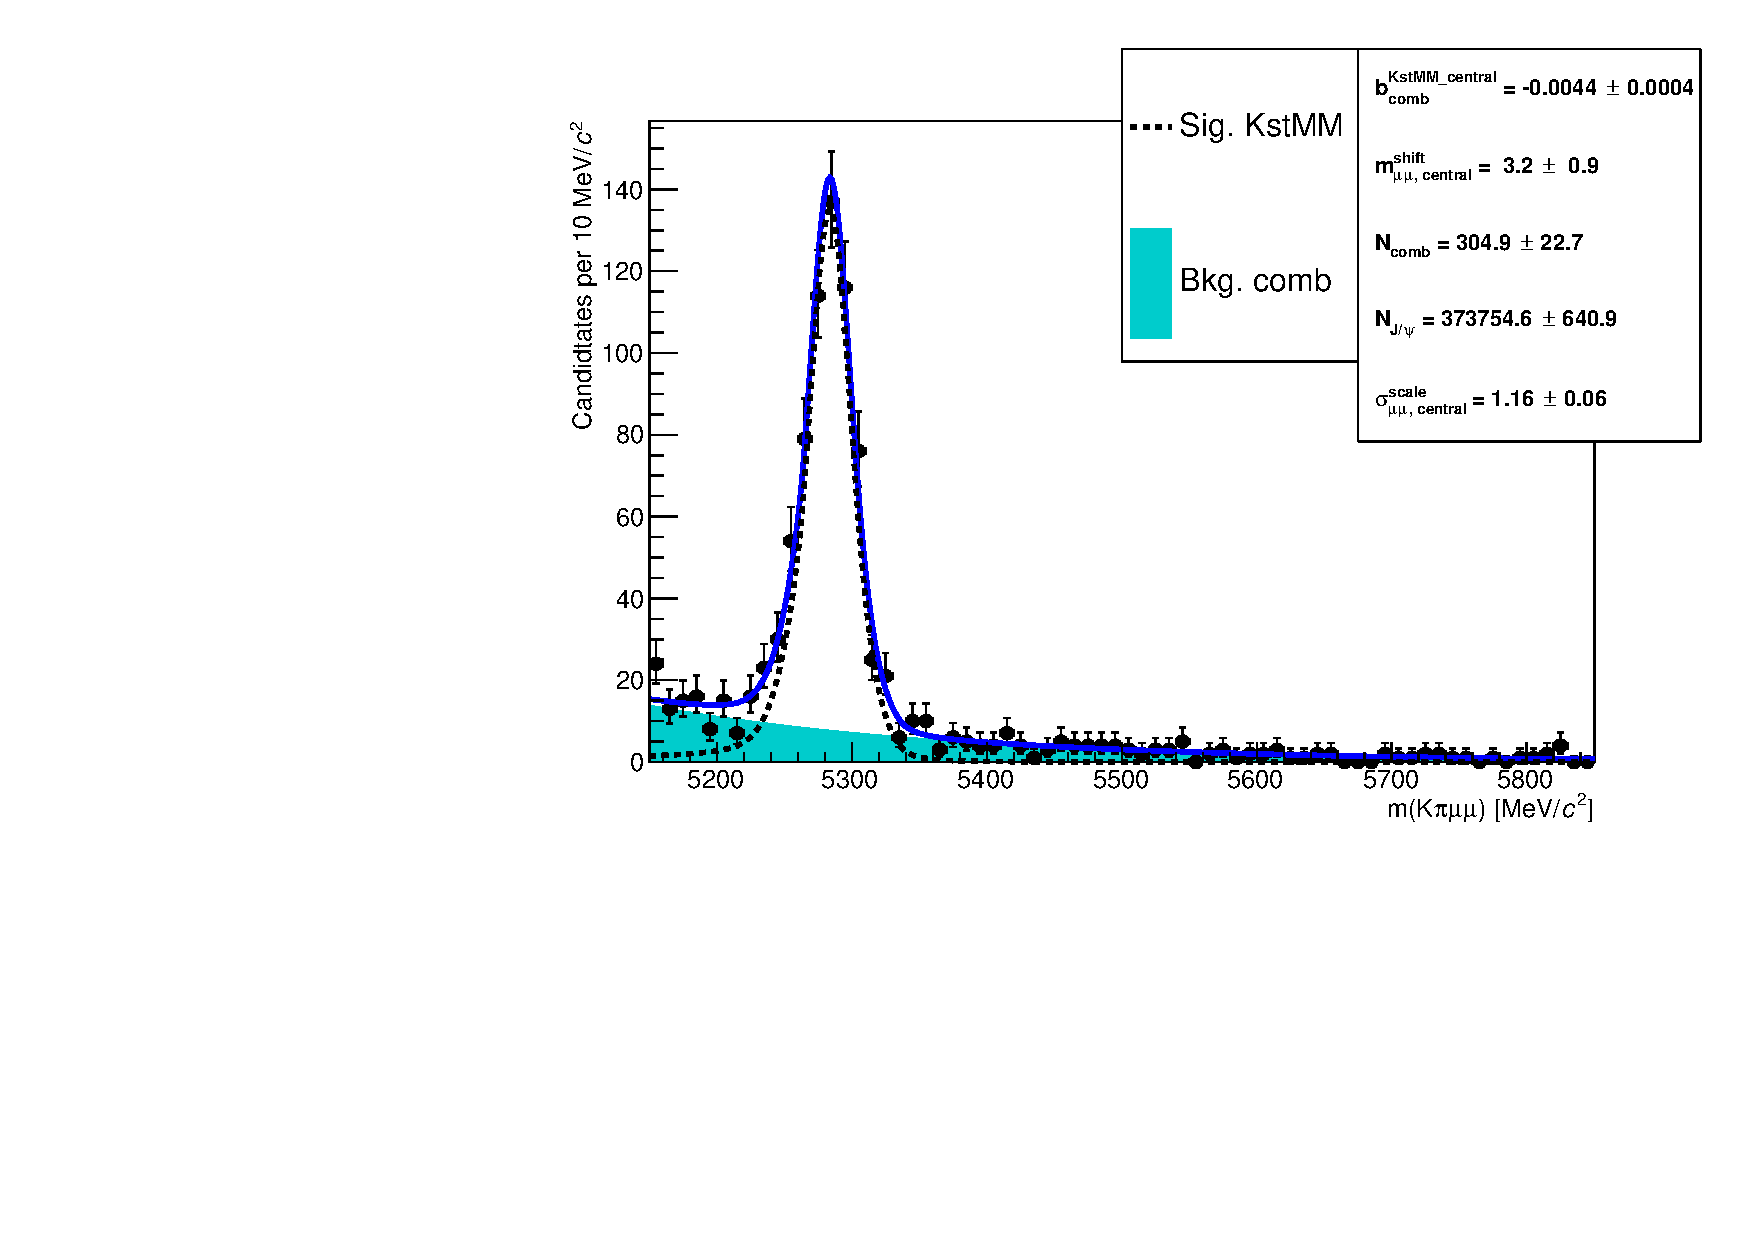
\includegraphics[width=0.55\textwidth]{RKst/figs/Fit/fit_MM/KstMM_central.pdf}
%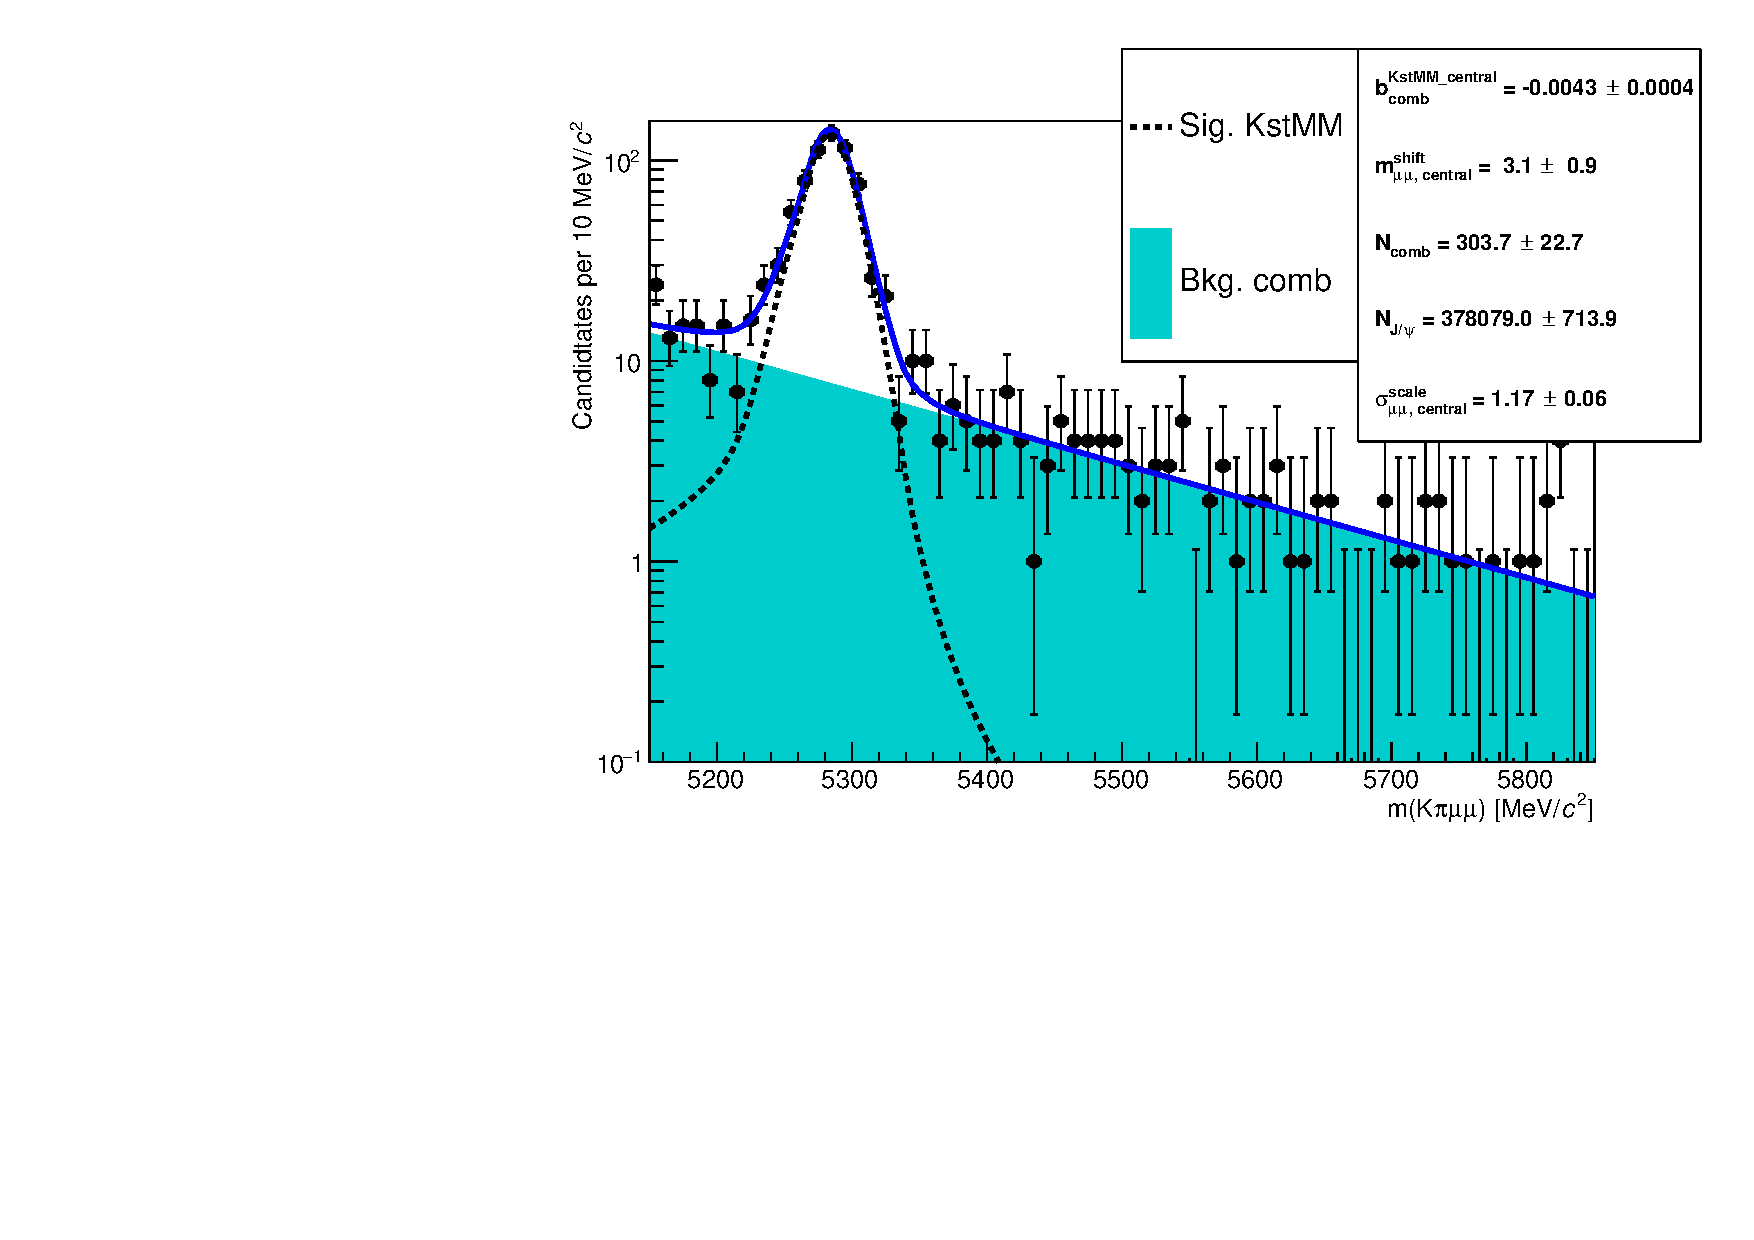
\includegraphics[width=0.49\textwidth]{RKst/figs/Fit/fit_MM/KstMM_central_log.pdf}
%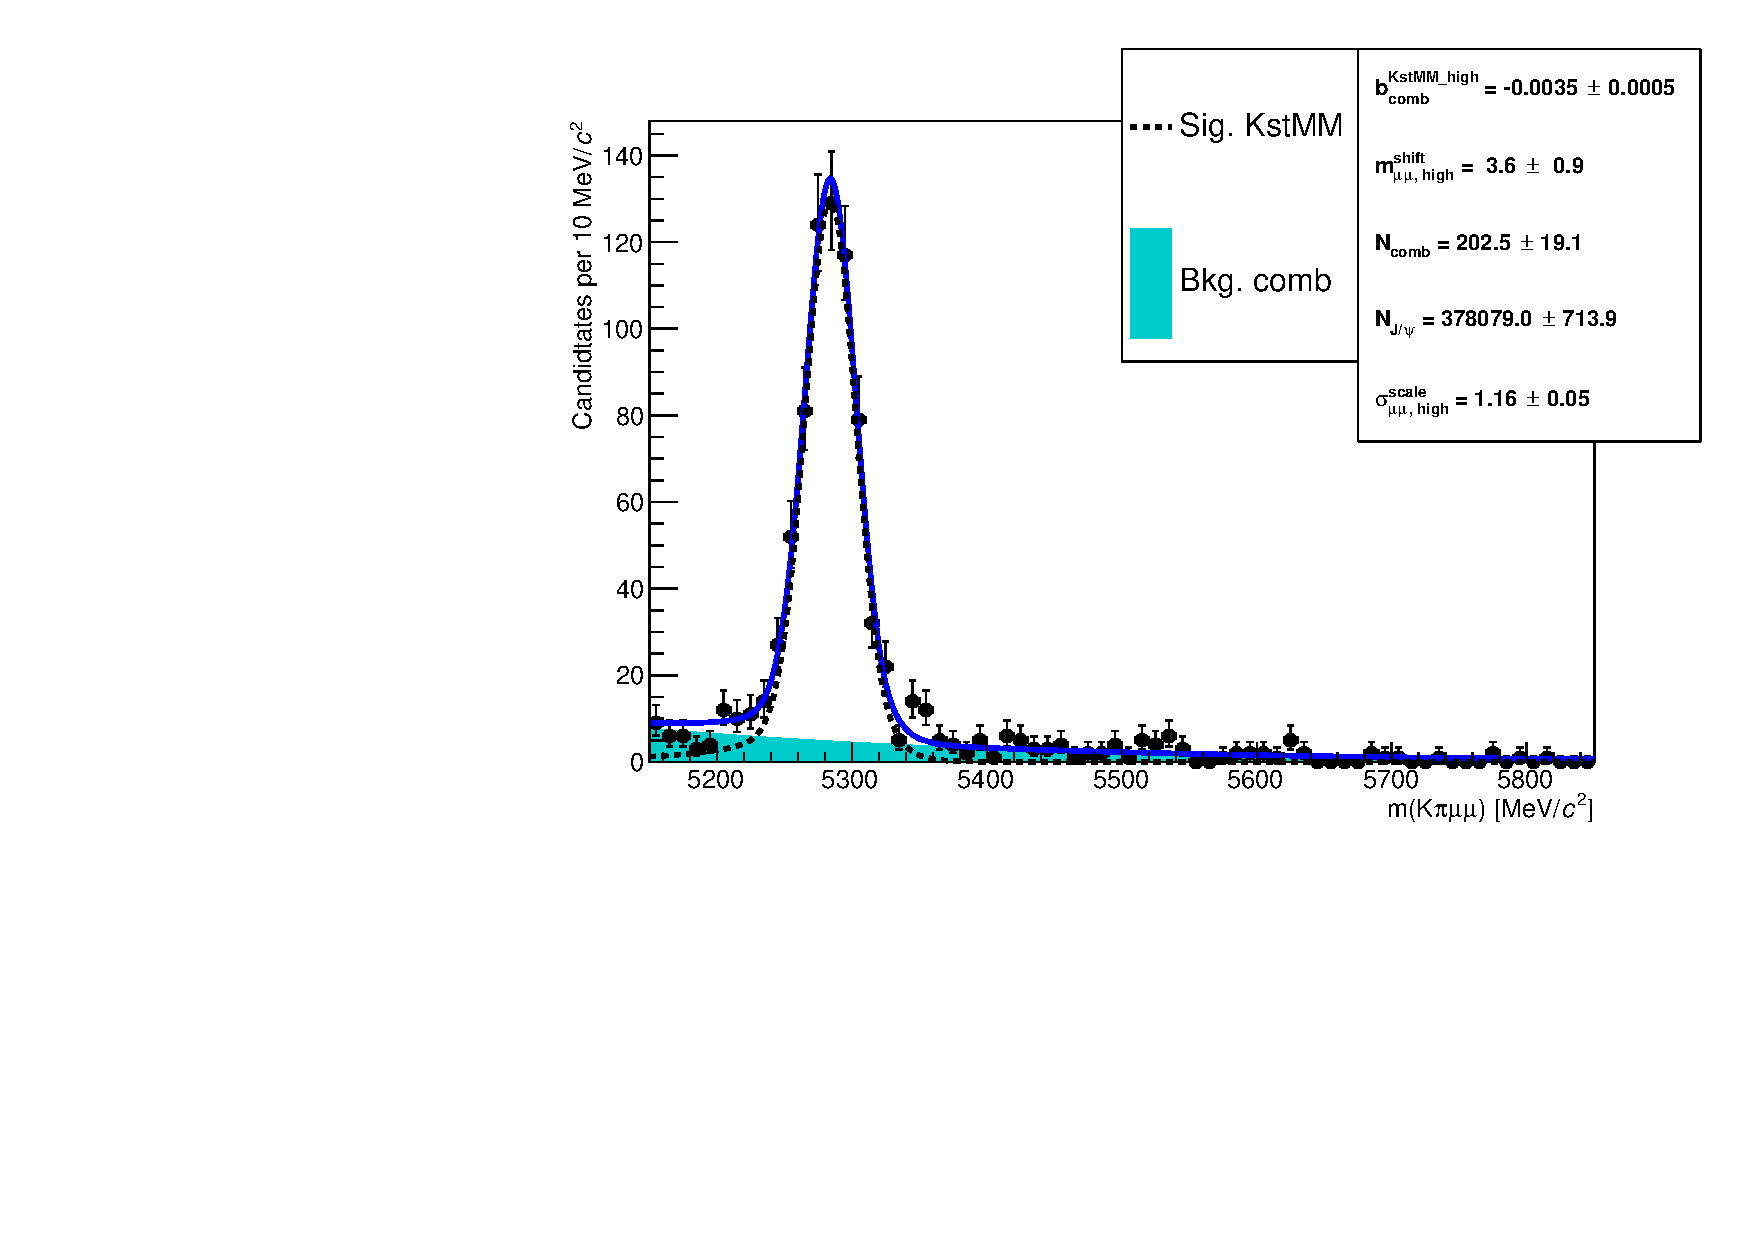
\includegraphics[width=0.55\textwidth]{RKst/figs/Fit/fit_MM/KstMM_high.pdf}
%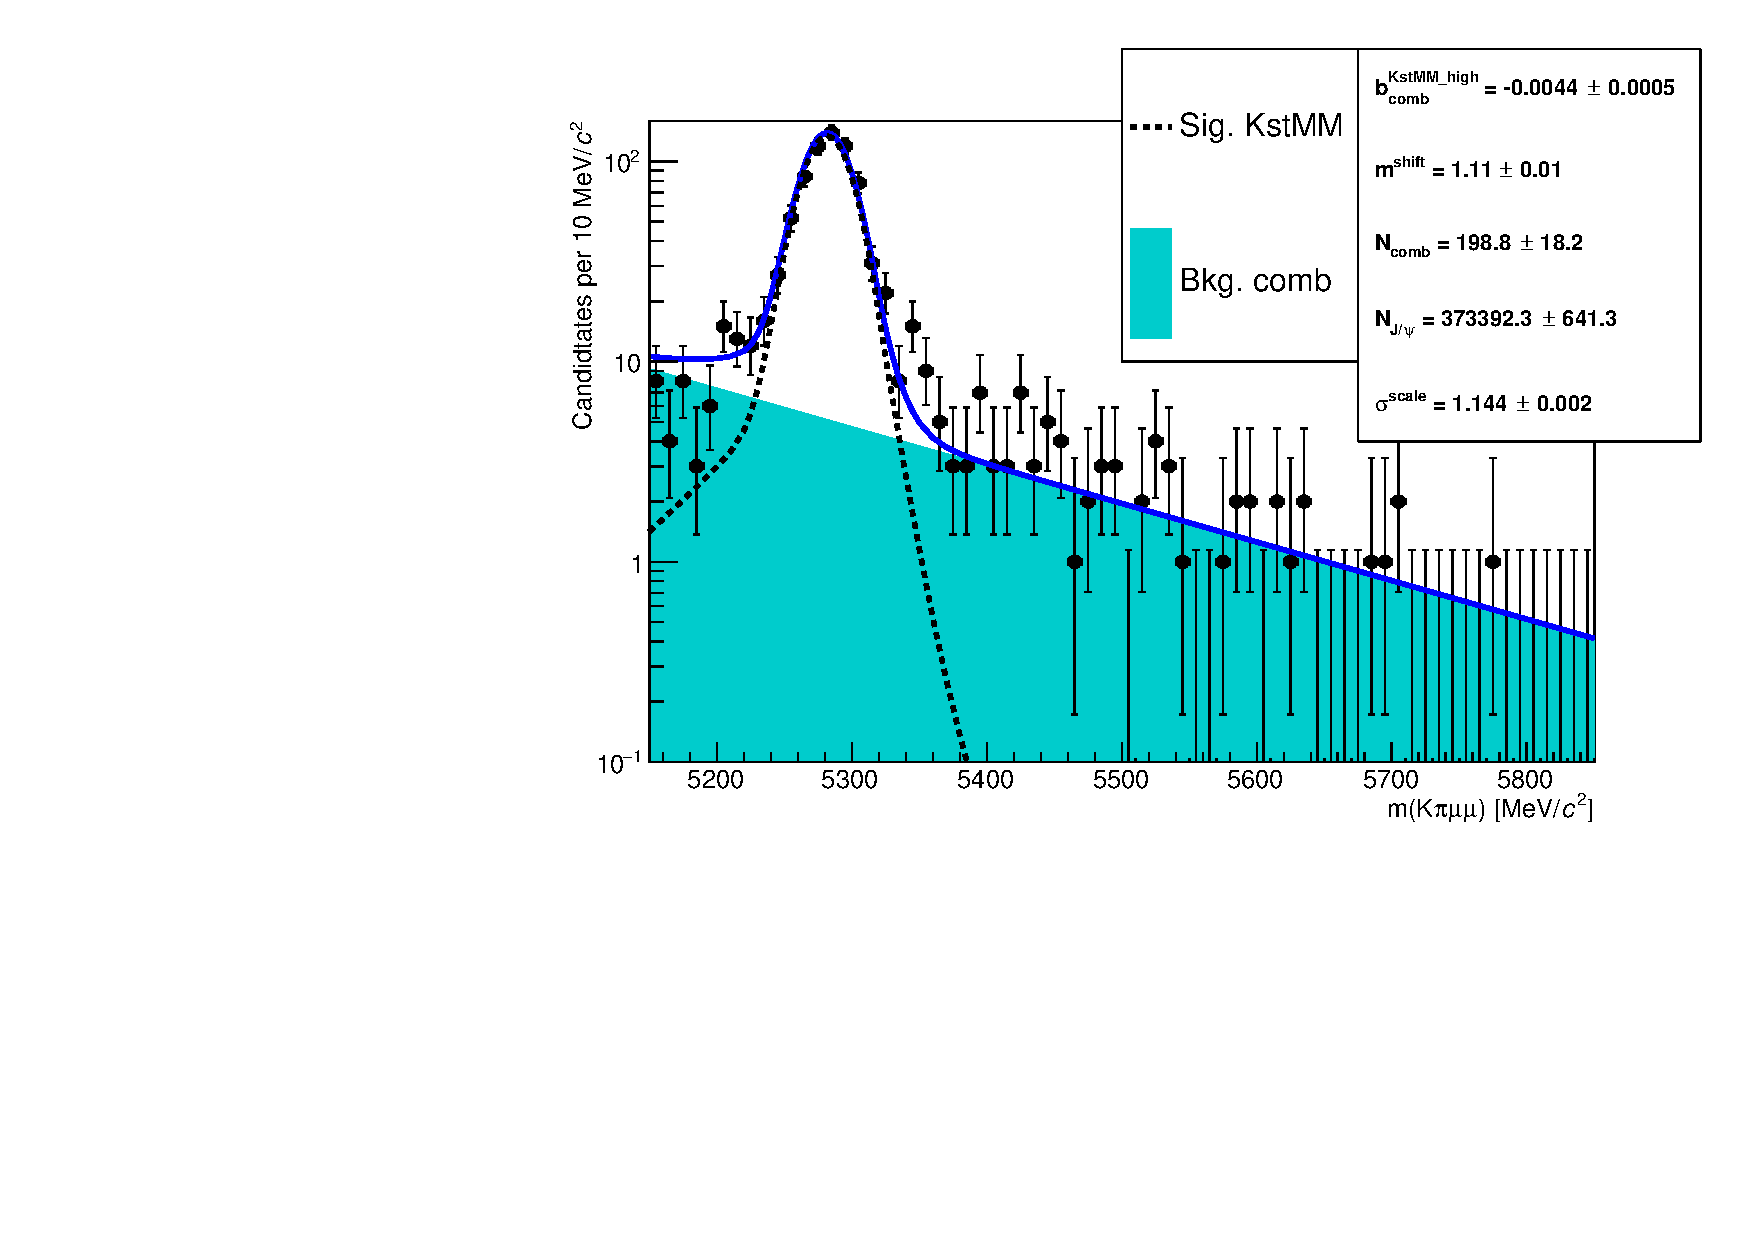
\includegraphics[width=0.49\textwidth]{RKst/figs/Fit/fit_MM/KstMM_high_log.pdf}
\caption{Fitted $m(K\pi \mu\mu)_\jpsi$ invariant mass distribution for $\jpsi(\mu\mu)$ candidates
in logarithmic scale. Dashed black lines represent the signal PDFs and filled shapes the background components. }
\label{fig:mumu_data_fits}
\end{figure}
%
\begin{figure}[h!]
\centering
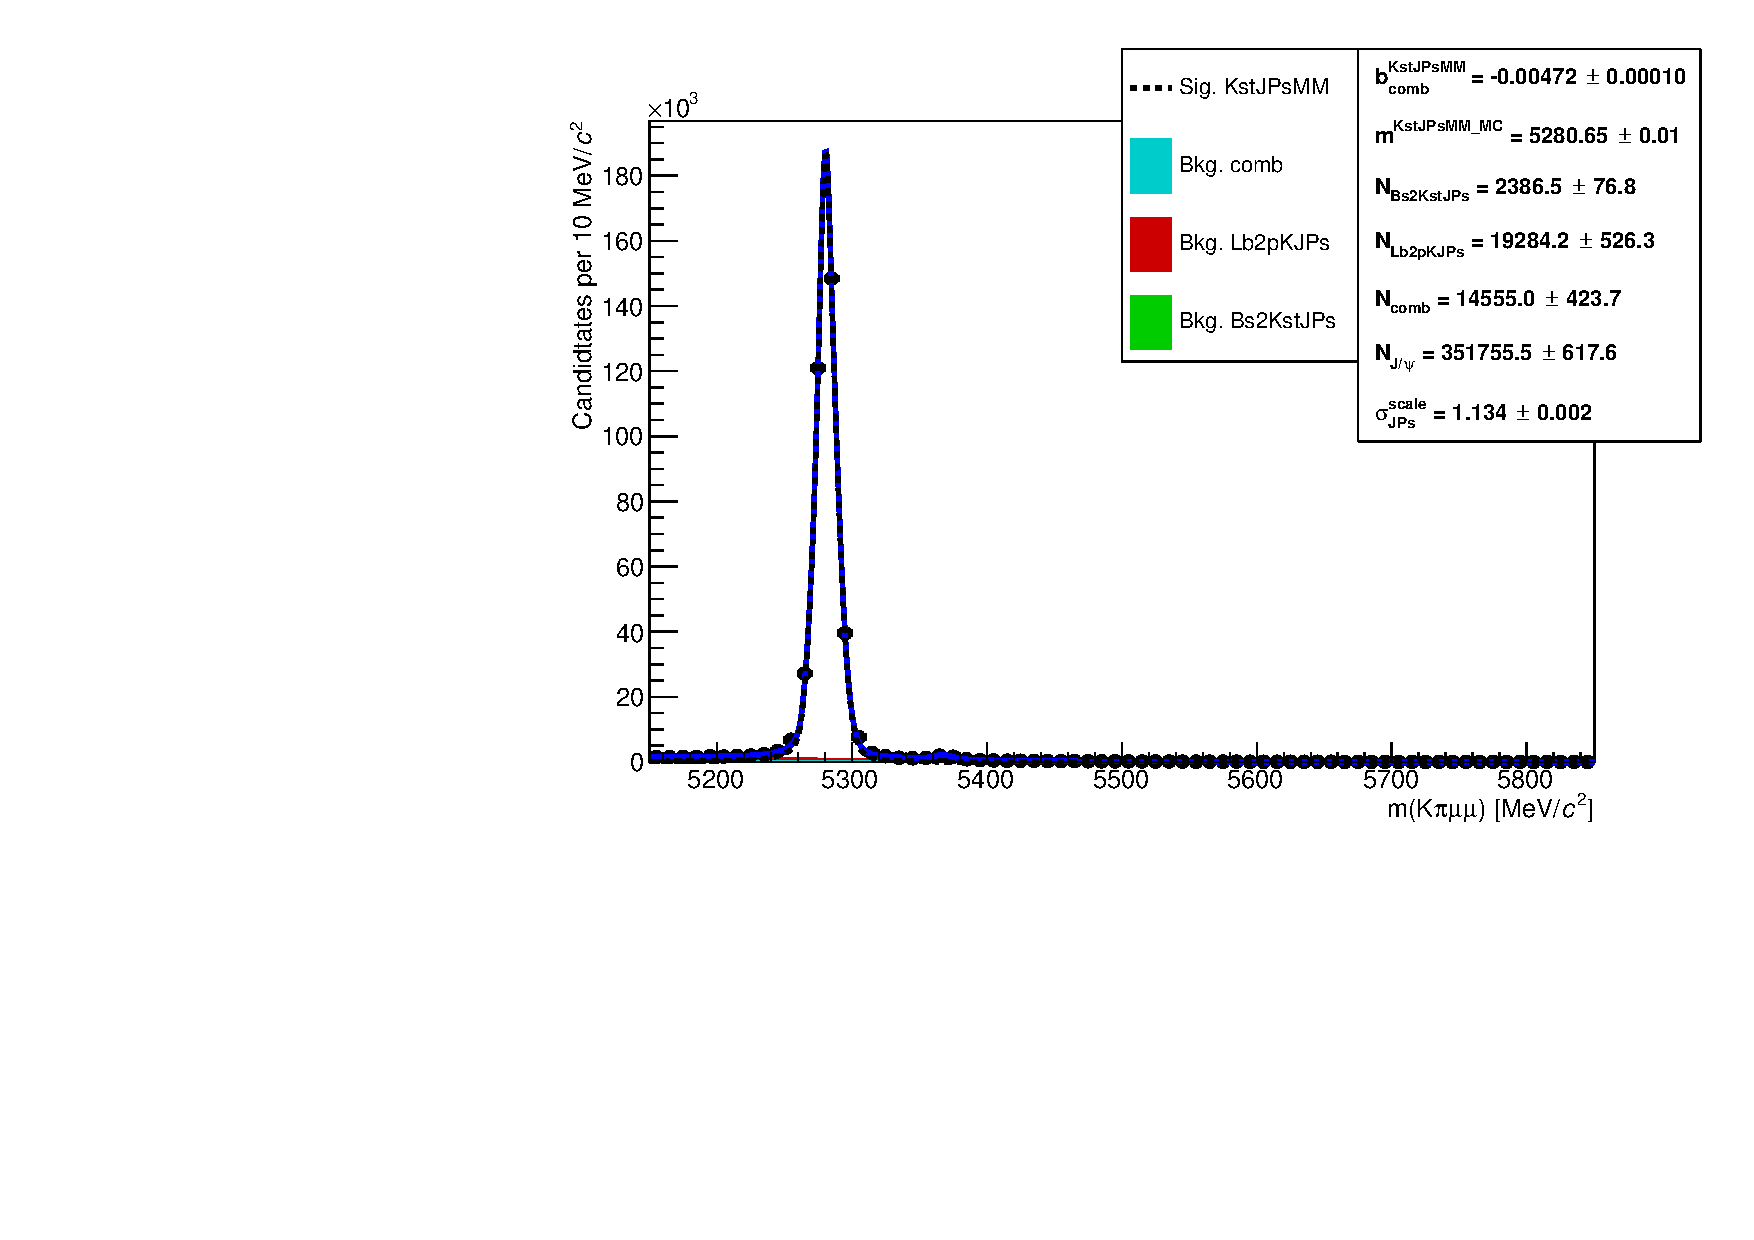
\includegraphics[width=0.49\textwidth]{RKst/figs/Fit/fit_MM/KstJPsMM.pdf}
%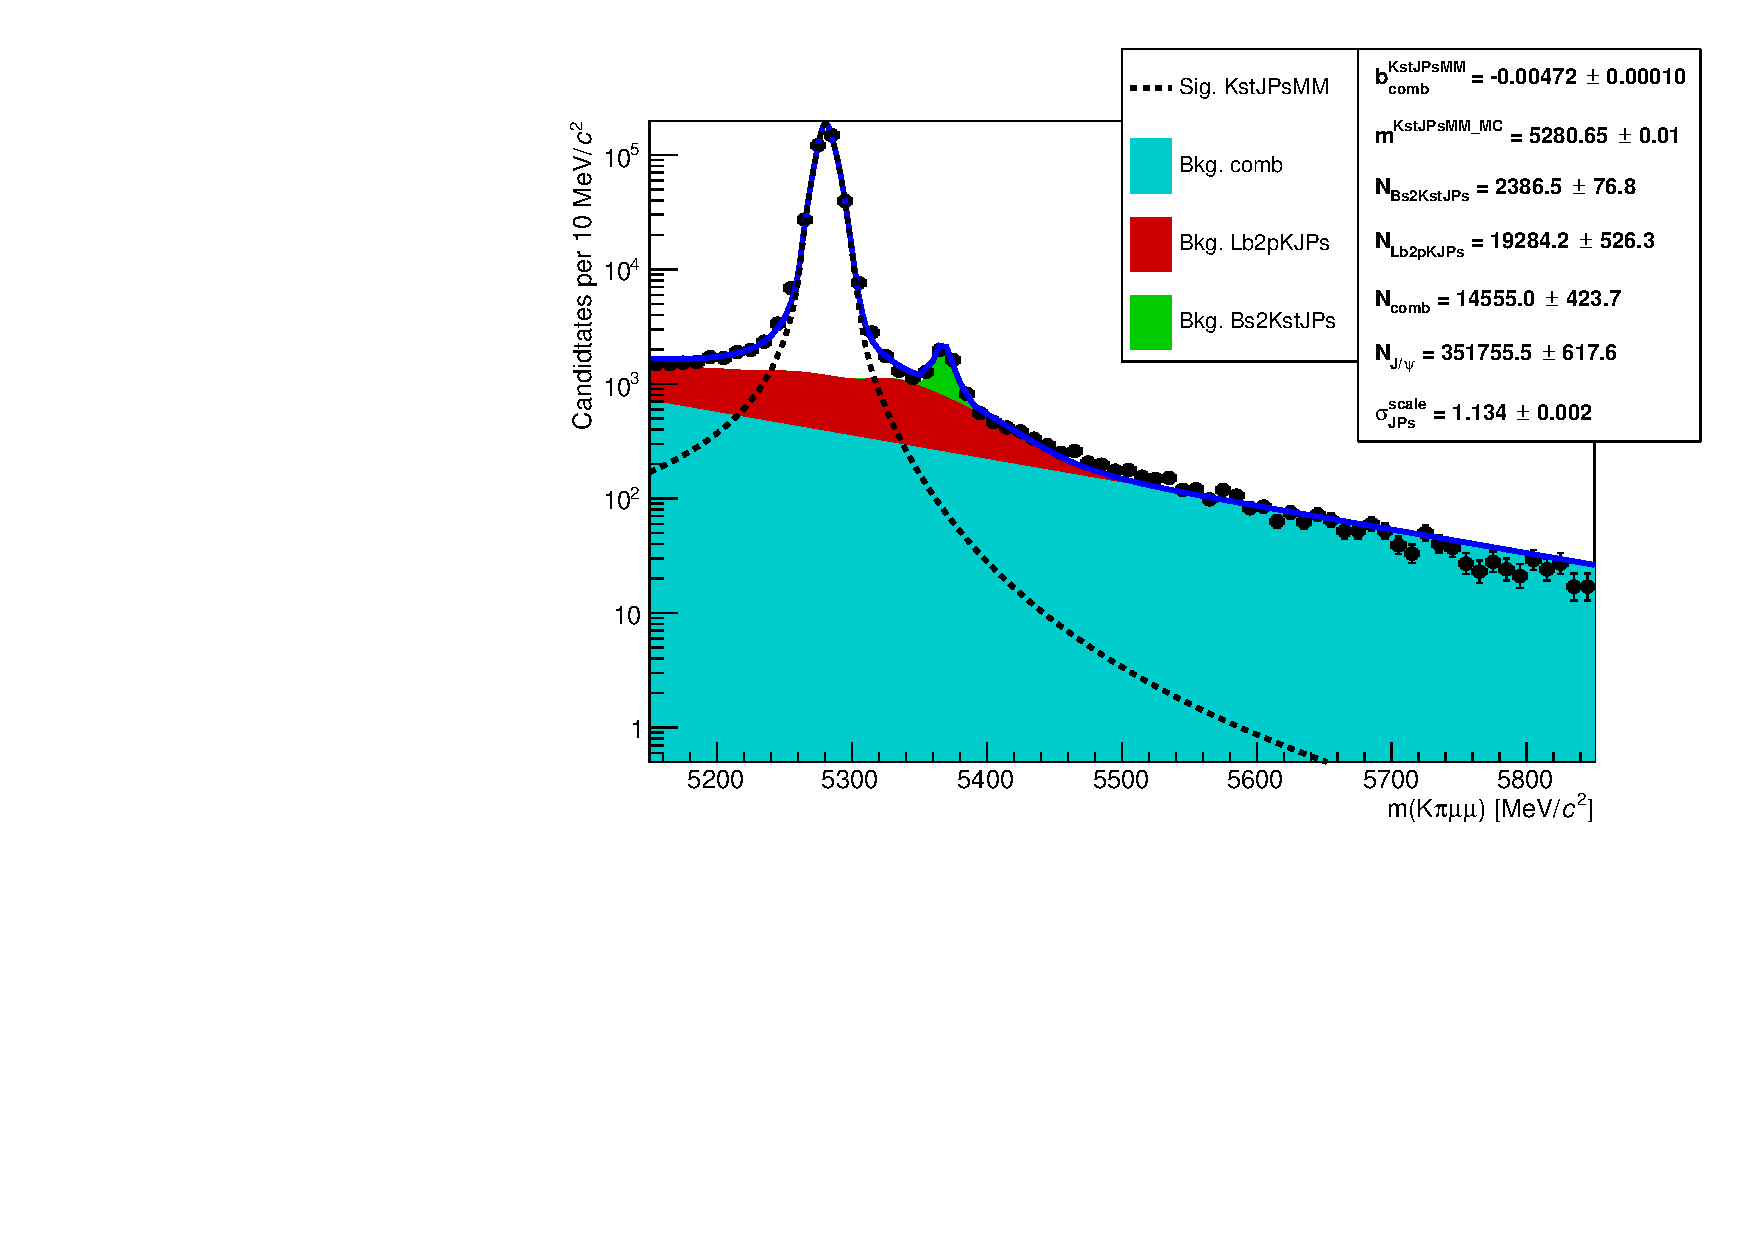
\includegraphics[width=0.49\textwidth]{RKst/figs/Fit/fit_MM/KstJPsMM_log.pdf}
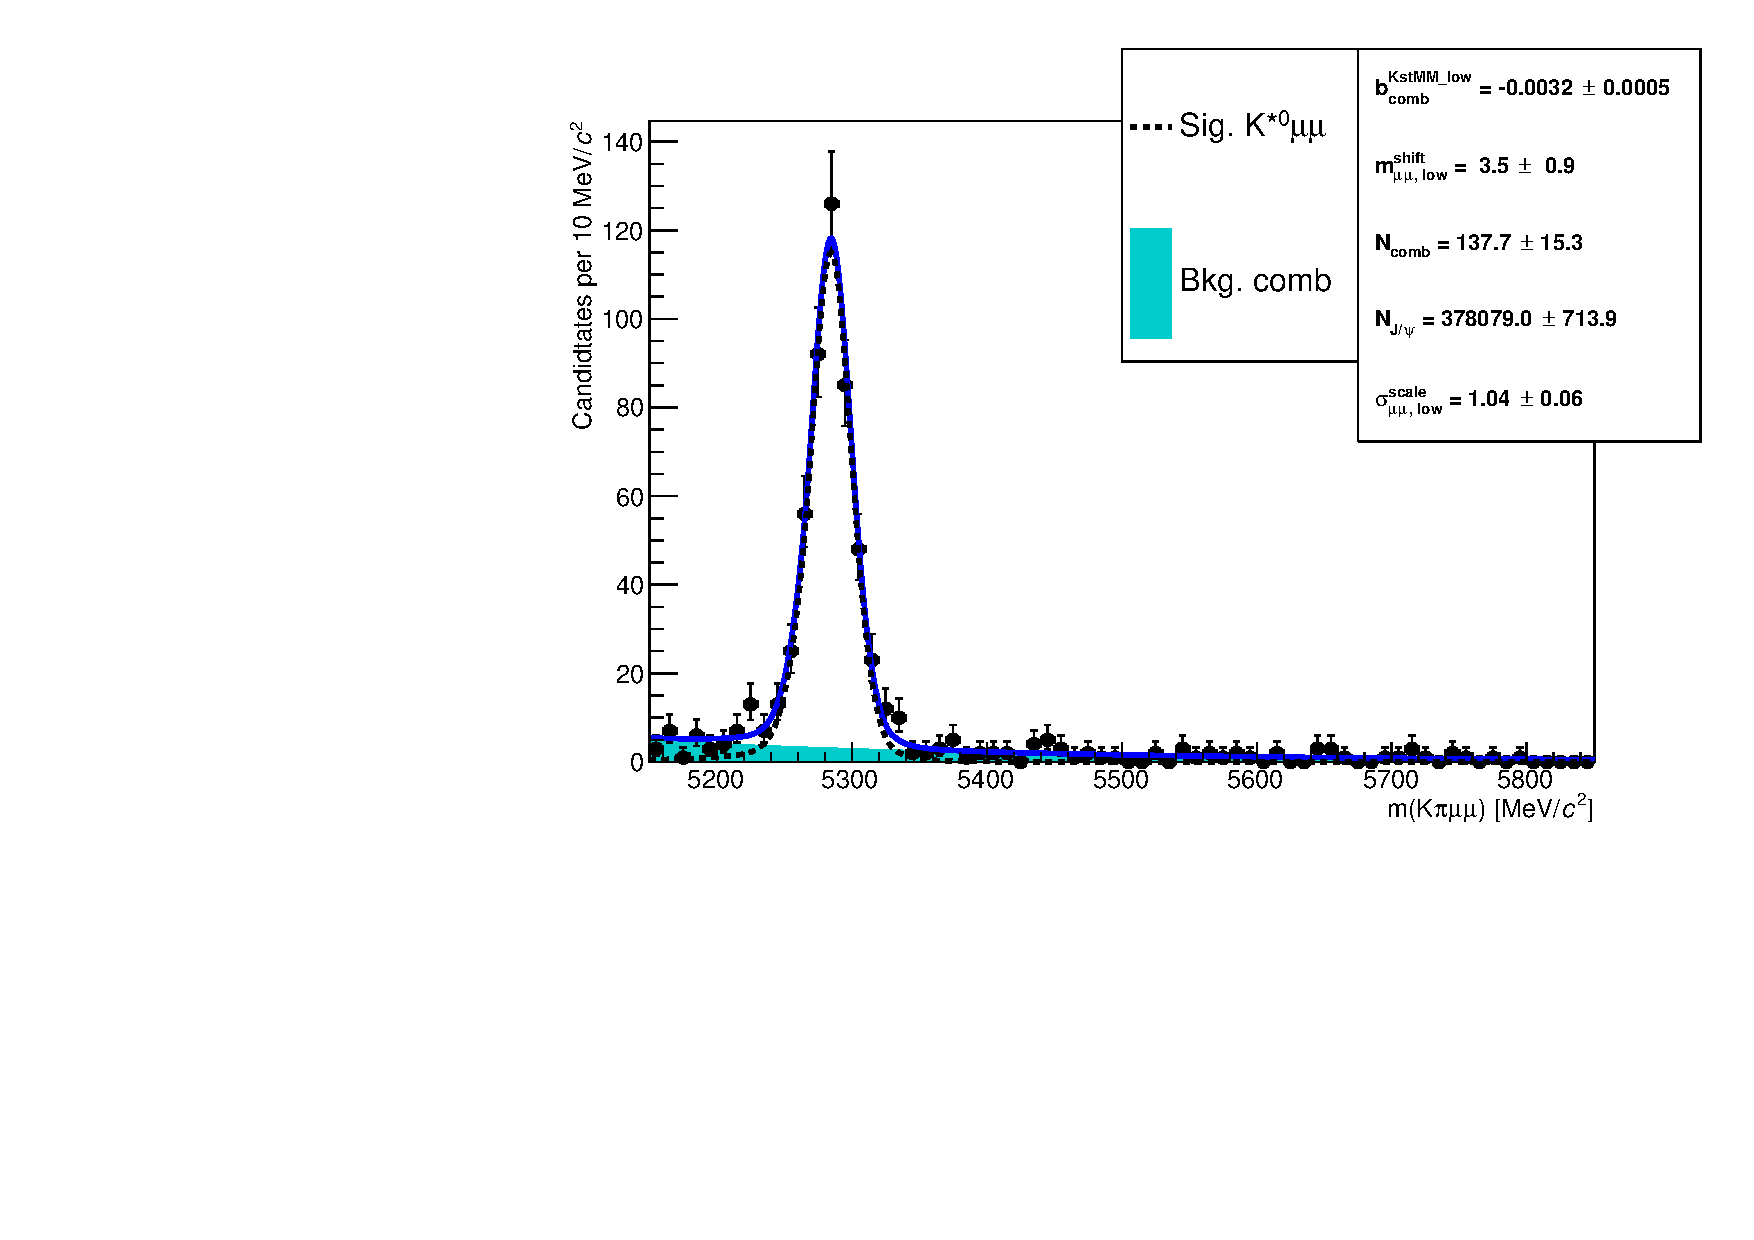
\includegraphics[width=0.55\textwidth]{RKst/figs/Fit/fit_MM/KstMM_low.pdf}
%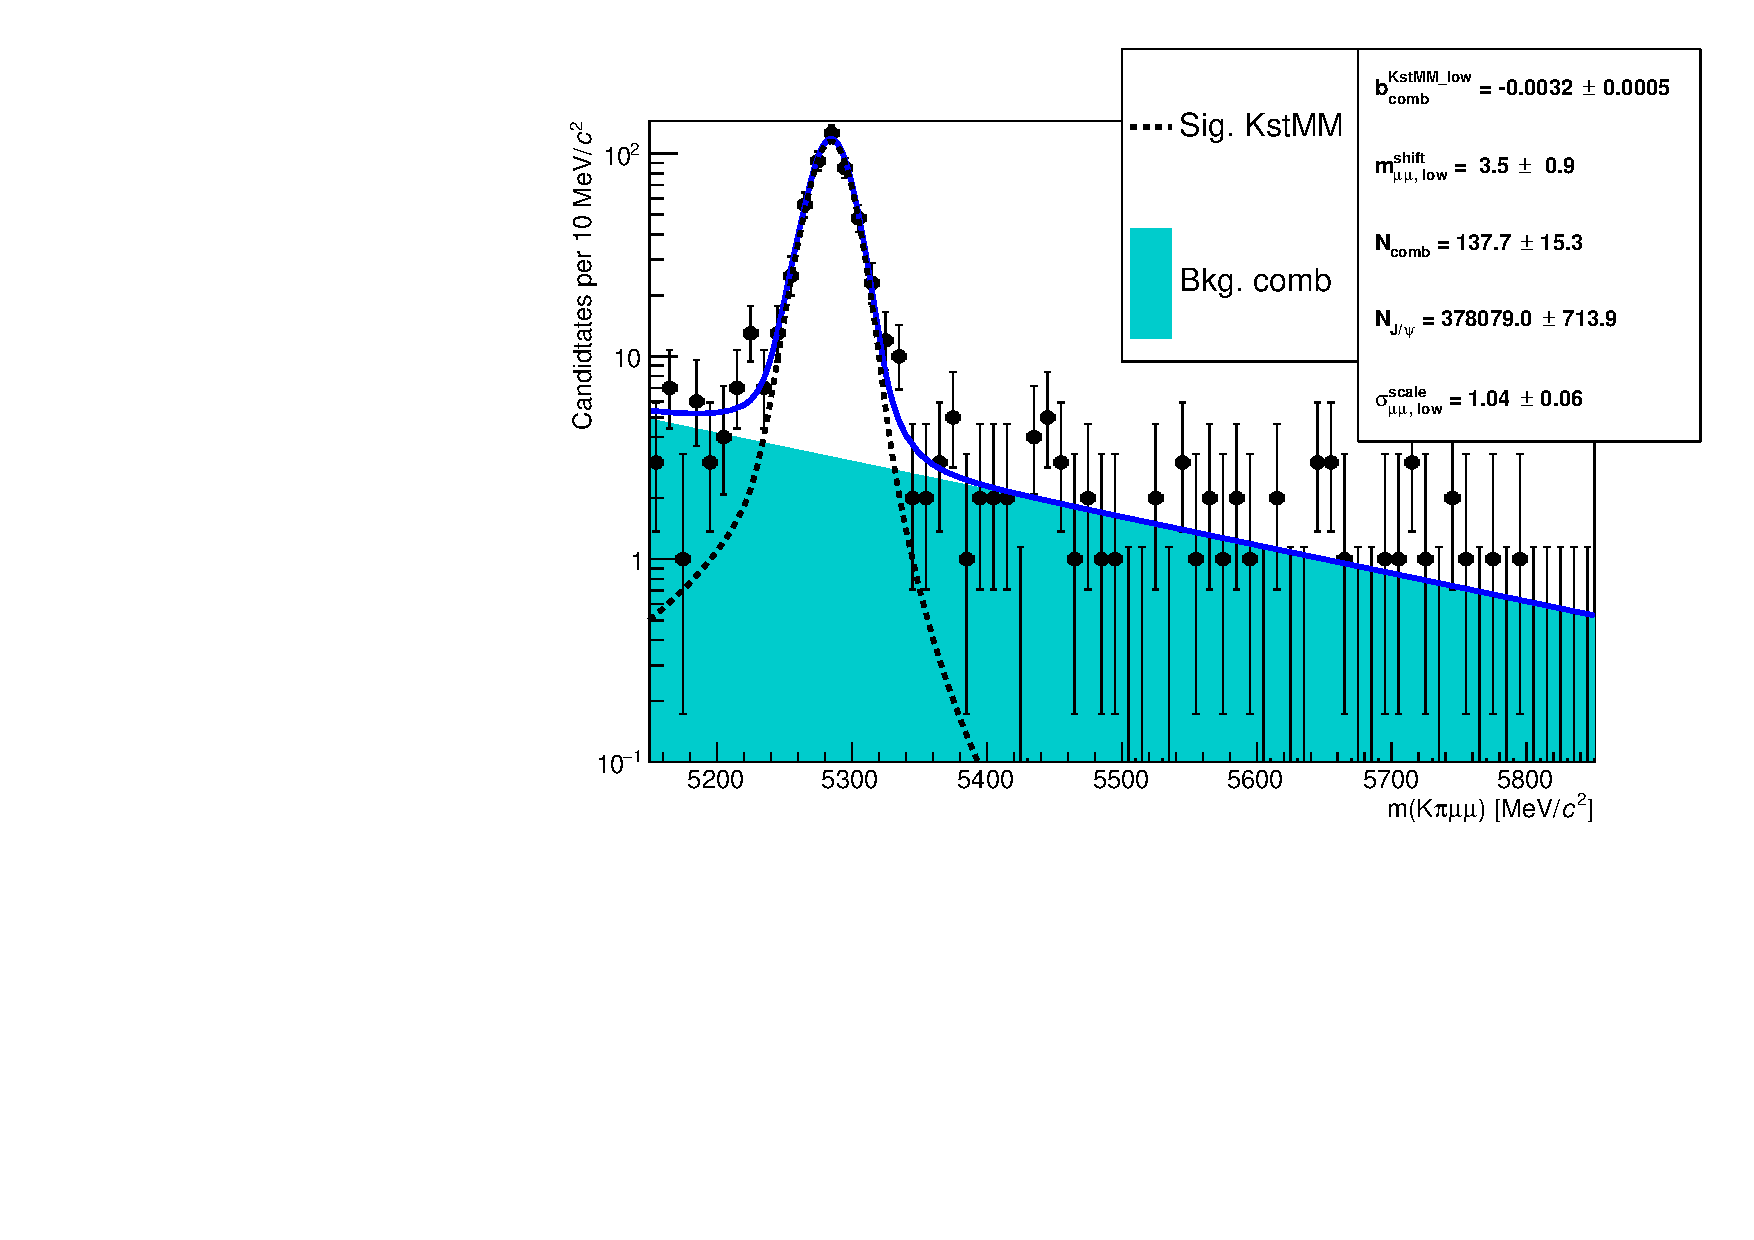
\includegraphics[width=0.49\textwidth]{RKst/figs/Fit/fit_MM/KstMM_low_log.pdf}
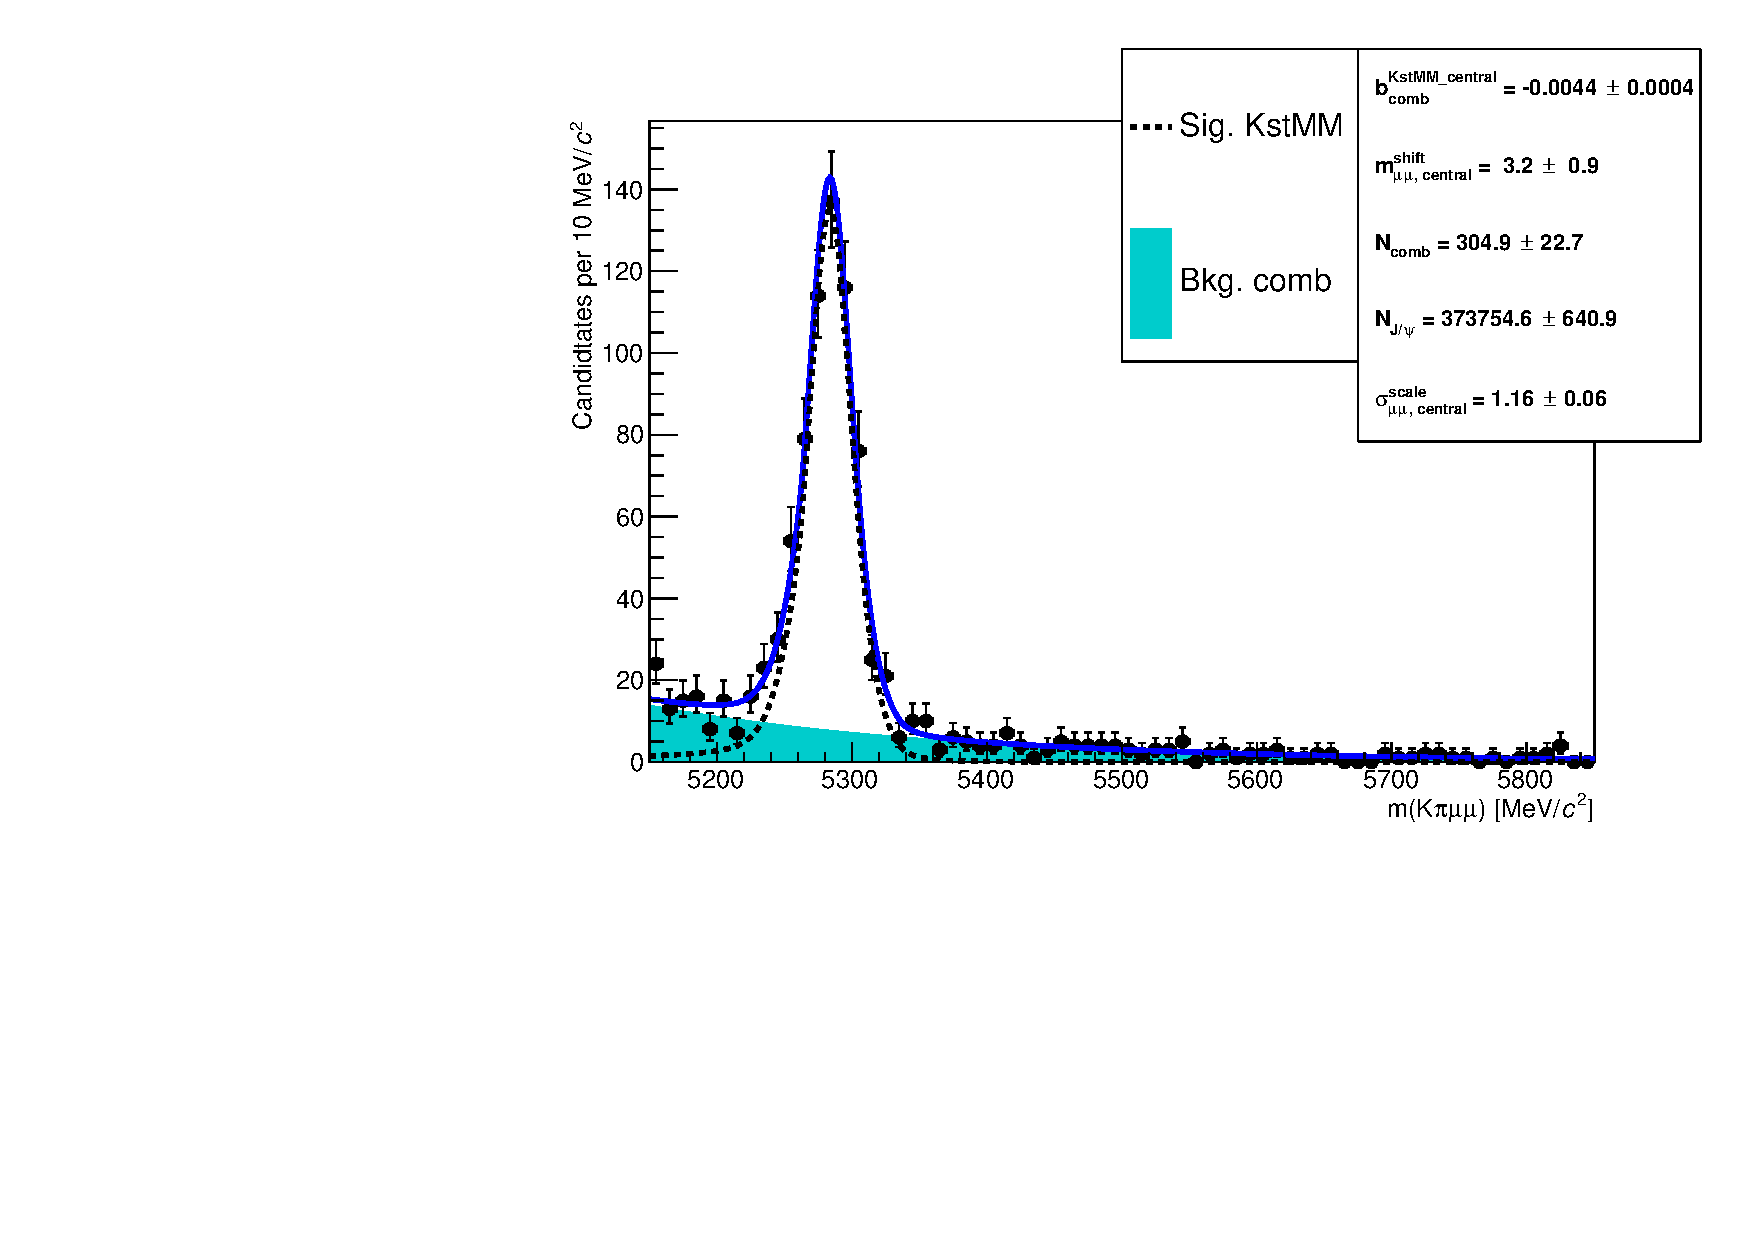
\includegraphics[width=0.55\textwidth]{RKst/figs/Fit/fit_MM/KstMM_central.pdf}
%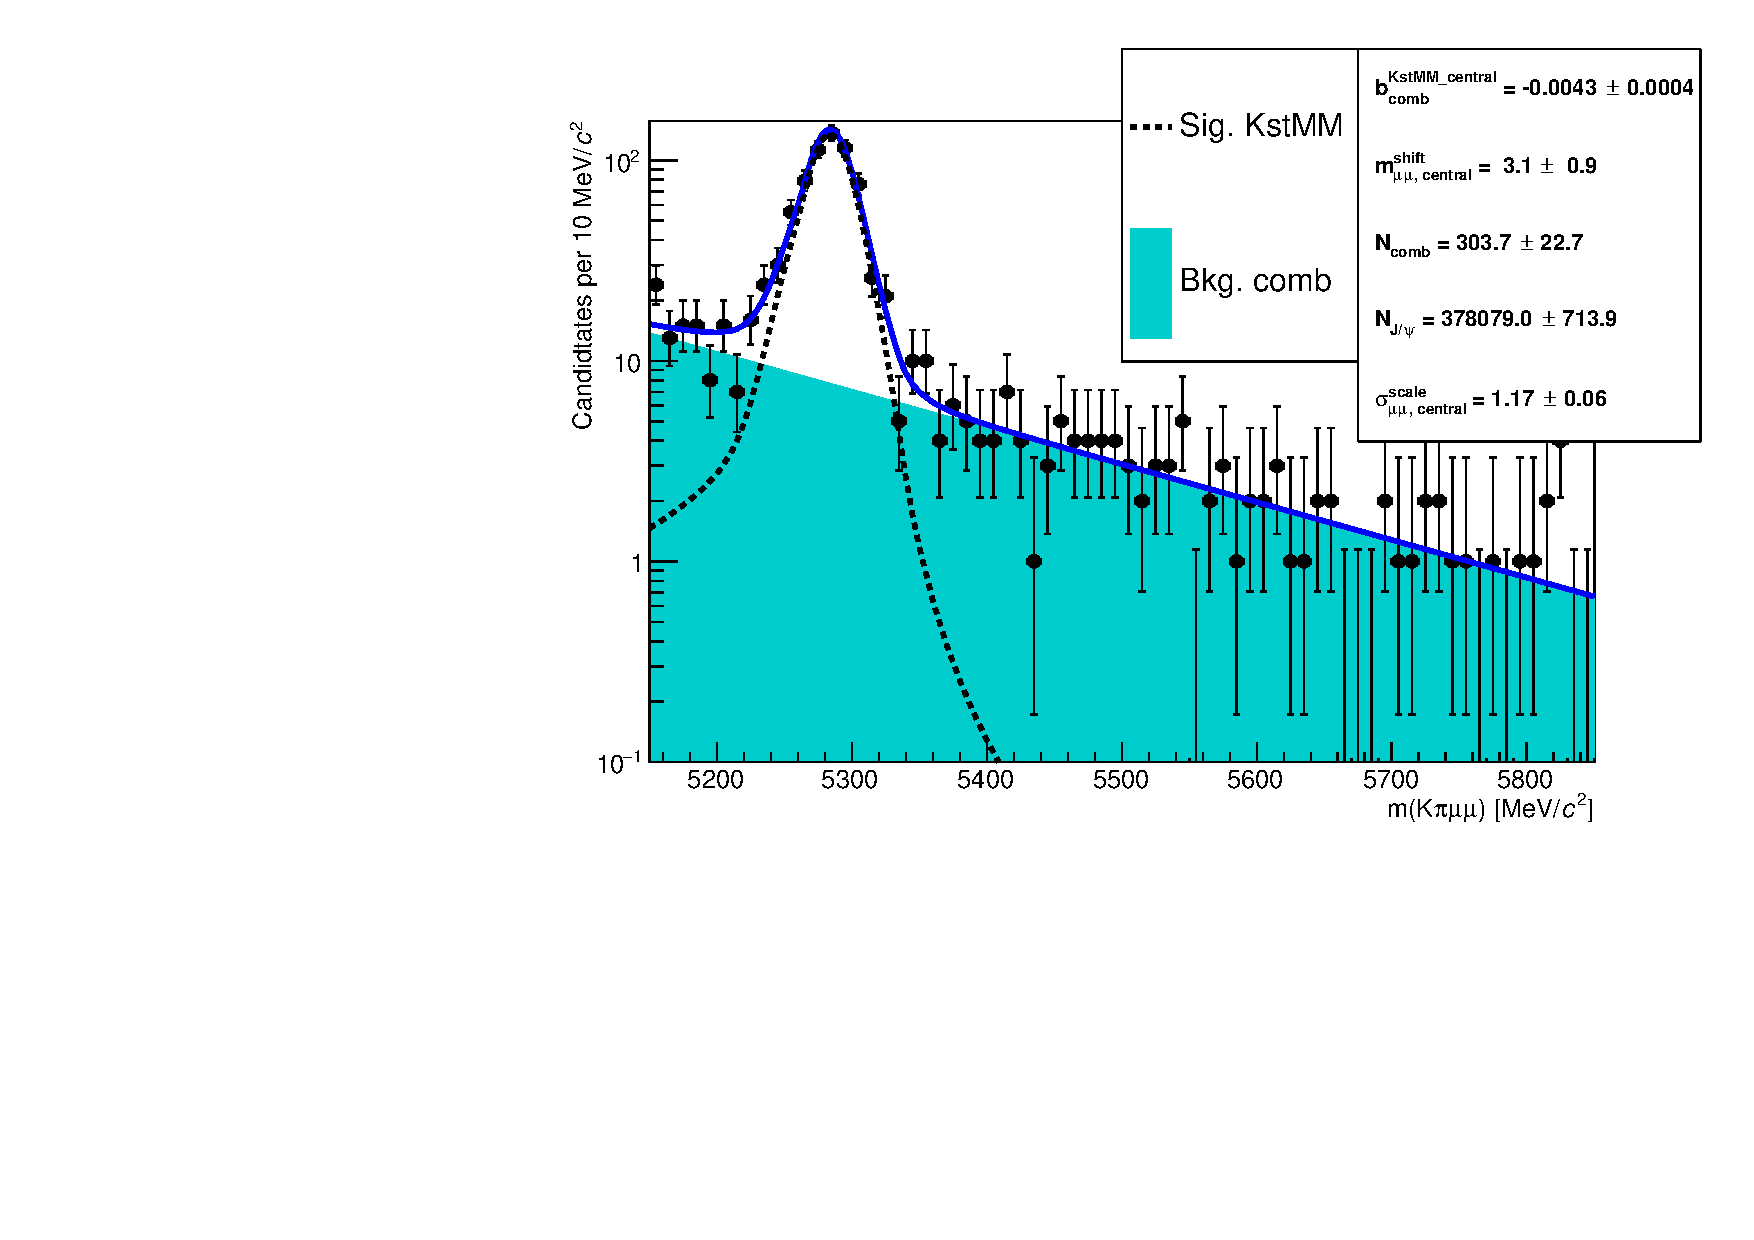
\includegraphics[width=0.49\textwidth]{RKst/figs/Fit/fit_MM/KstMM_central_log.pdf}
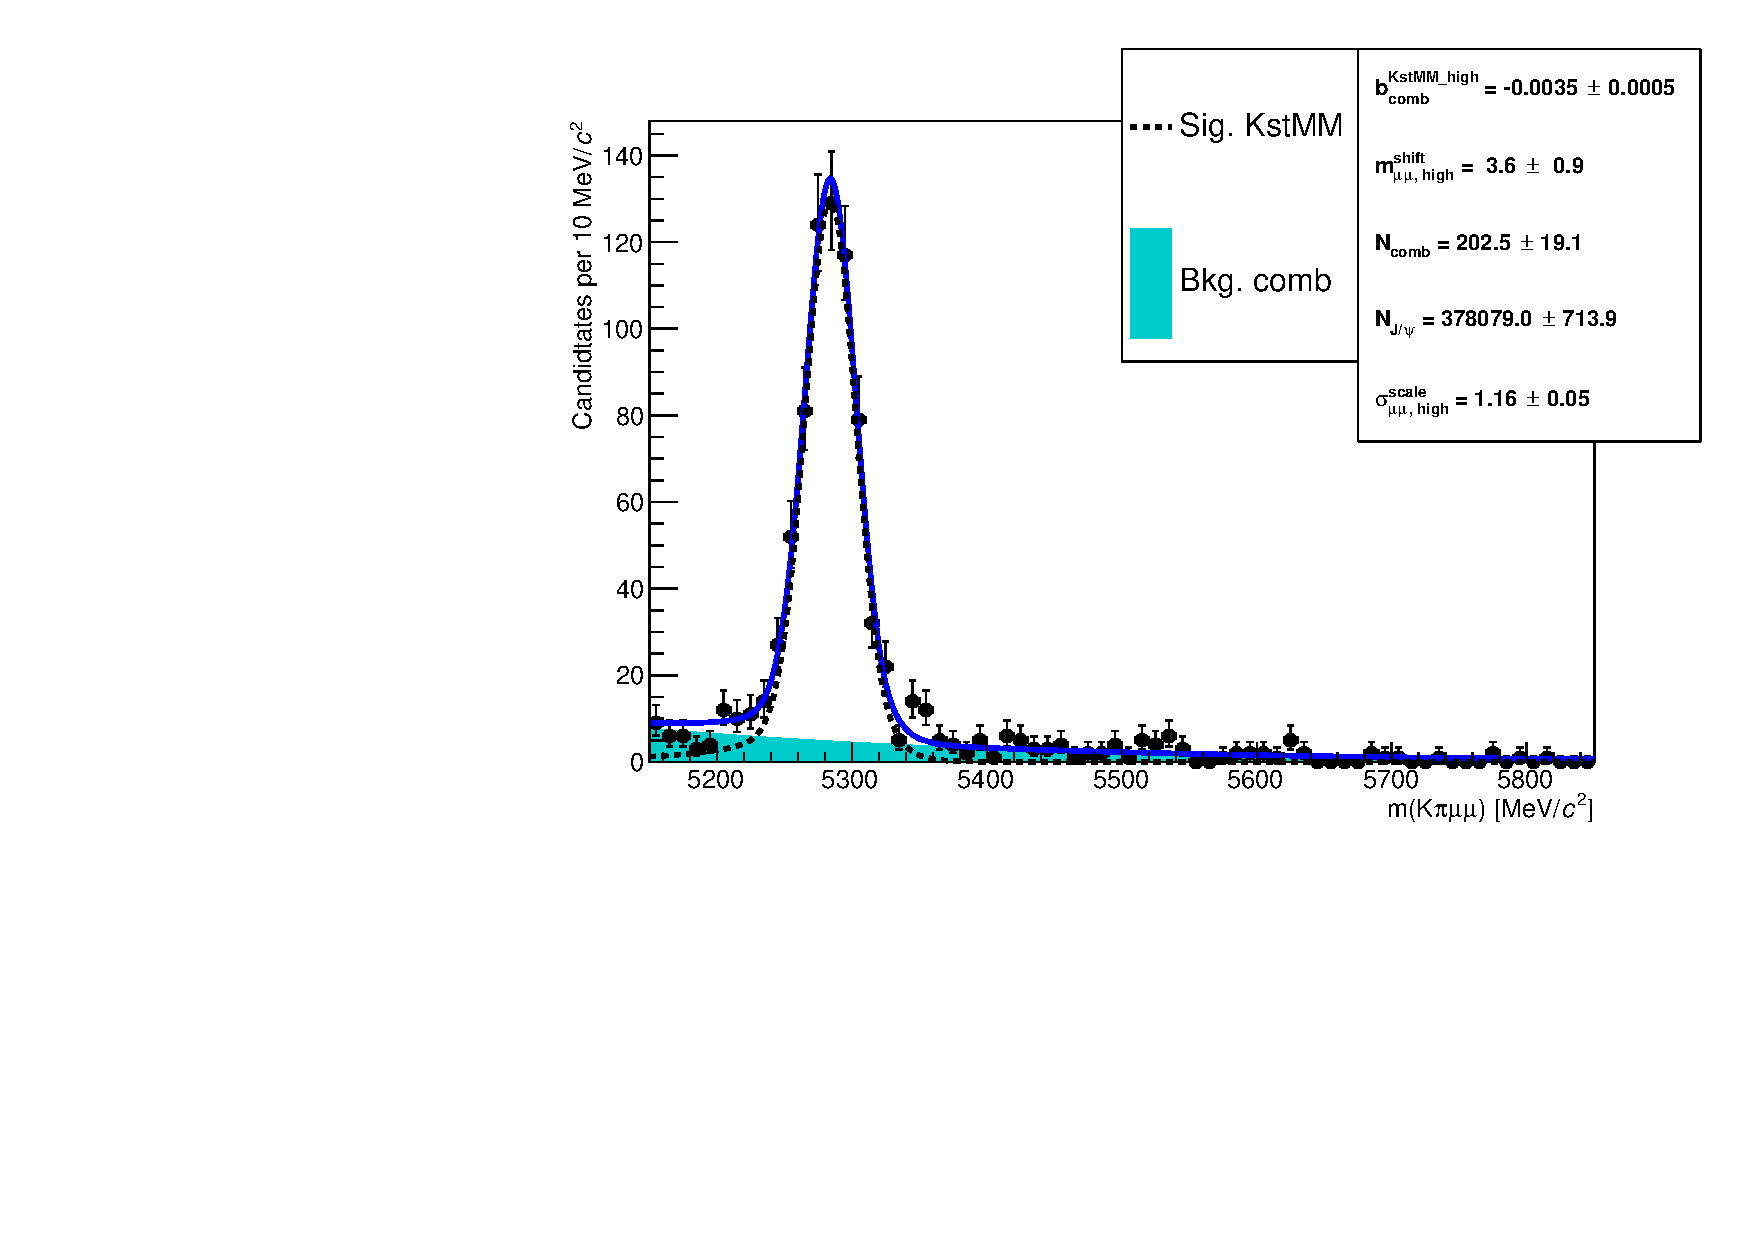
\includegraphics[width=0.55\textwidth]{RKst/figs/Fit/fit_MM/KstMM_high.pdf}
%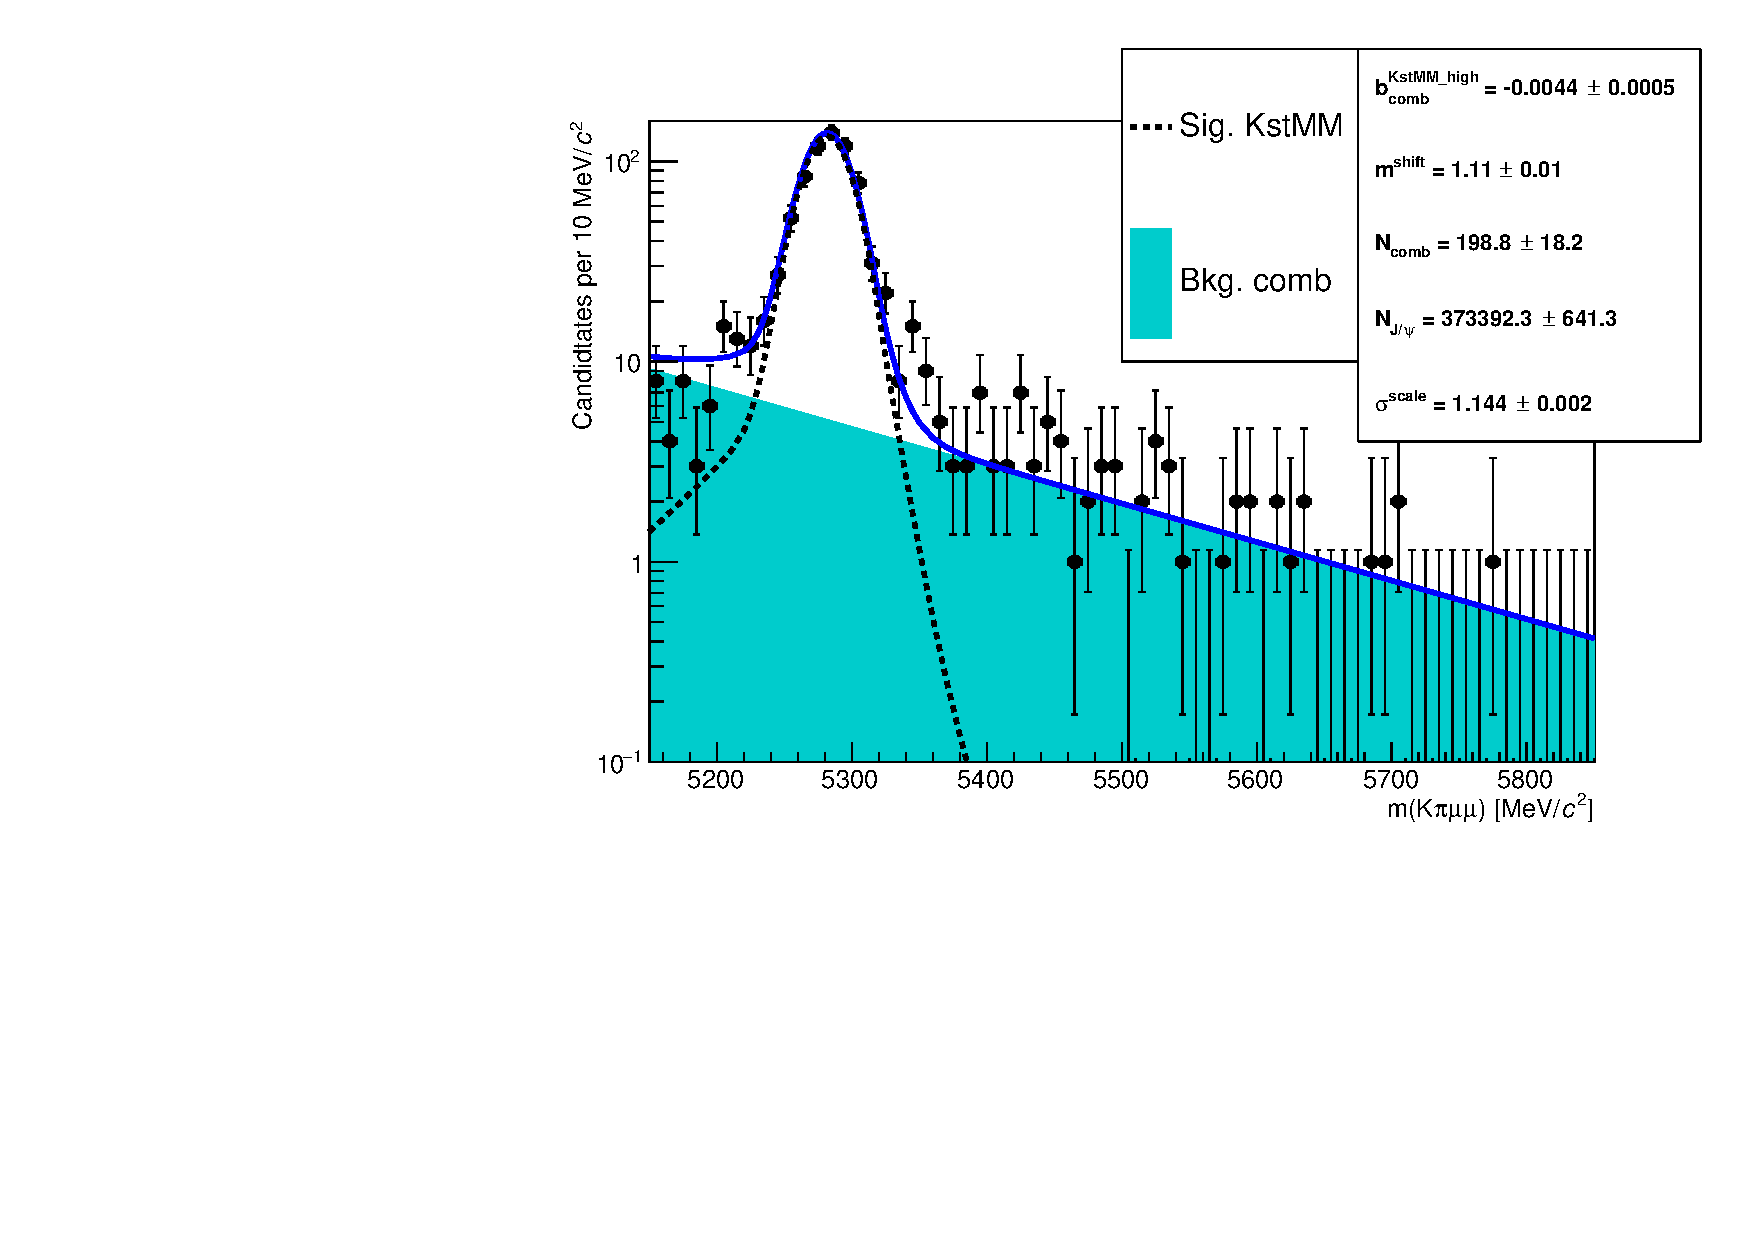
\includegraphics[width=0.49\textwidth]{RKst/figs/Fit/fit_MM/KstMM_high_log.pdf}
\caption{From top to bottom fitted $m(K\pi \mu\mu)_\jpsi$ invariant mass distributions
 for $\jpsi(\mu\mu)$ candidates and fitted $m(K\pi \mu\mu)$ distributions for rare candidates 
 in the low-, central- and high-\qsq intervals. Dashed black lines represent the signal PDFs and 
 filled shapes the background components. }
\label{fig:mumu_data_fits}
\end{figure}

\clearpage

\subsection{Electron channels}
\label{sec:RKst_fit_ee}

Also in the electron case the fitted variable is the 4-body invariant mass coming from a kinematic fit.
In general, this does no include constraints to intermediate resonances, unless specified.
When constraints to intermediate resonances are applied the invariant mass is referred to as
$m(K\pi ee)_R$, where $R = \jpsi$ or \psitwos.
%The reconstructed invariant mass of the \Bz depends on which L0 line triggered the event.
A simultaneous fit to the 4-body invariant mass of the \BdToKstJPsee and \BdToKstee 
channels and across the three trigger categories defined in Sec.~\ref{sec:RKst_trigstripping} is performed.
%
For each trigger category, the $\jpsi(ee)$ and $ee$ yields are extracted from the following signal channel categories:
%
\begin{itemize}
\item \BdToKstJPsee, with a \jpsi mass constraint, $m(K\pi ee)_{\jpsi}$;
\item \BdToKstee in the three \qsq intervals.
\end{itemize}

Extra control channels are fit simultaneously:
%
\begin{itemize}
\item \BdToKstGee to constrain the yield of partially-reconstructed background 
in the low-\qsq and the leakage of \BdToKstG into the low-\qsq;
\item \BdToKstJPsee, without the \jpsi mass constraint, to constrain the leakage into the central-\qsq and the 
parameters that model residual data-simulation discrepancies;
\item \BdToKstPsiee, with a \psitwos mass constraint,  $m(K\pi ee)_{\psi}$, to constrain the leakage to lower and higher \qsq values.
\end{itemize}

When fitting the variable without a \jpsi mass constraint it is important to fit a wider mass range to better constrain the 
parameters modelling the radiative tail and the backgrounds; therefore a mass window [4500,6200]~\mevcc~ is used. The lower limit 
is given by the point in which the \qsq cut (at 6~\gevgevcccc to separate the rare and resonant channels)
starts to affect the 4-body invariant mass distribution. 
%
%For the variable with a mass constraint a mass window of 5150--5850\mevcc is used to fit the \JPsee, which has the advantage of removing the contributions from the partially-reconstructed background.
%
%The control samples of \BdToKstPsiee and
%\BdToKstGee candidates are also added to the simultaneous fit and a few parameters are shared as explained later.
%Finally, for the \BdToKstJPsee candidates the invariant mass calculated without \jpsi mass constraint
%is also added to the fit as a control sample. This is necessary in order to obtain the data-simulation discrepancy parameters
%shared with the model for the rare samples, which requires to fit the same variable in both cases.

The invariant mass distributions are different depending on the
L0 line that triggered the event and also on the number of bremsstrahlung photons recovered.
%Furthermore the efficiencies can be more easily treated if divided in trigger categories.
Therefore, our samples are divided in three trigger categories, as described in
Sec.~\ref{sec:RKst_trigstripping}, and three bremsstrahlung categories defined as:
%
\begin{itemize}
\item $0\gamma$: candidates with no photons recovered;
\item $1\gamma$: candidates with one photon from either of the electrons;
\item $2\gamma$: candidates with more than one recovered photon.
\end{itemize}
%
All samples are fitted simultaneously, which allows a better use of the available statistics 
as the simultaneous fit gathers information from the three categories at the same time.
Furthermore, using this method the results for the three categories are
naturally combined in a single $r_{ee}$ ratio.
%
The PDFs used to fit the invariant mass distributions are described in the following sections.



\subsubsection{Signal PDFs for the electron channels}
\label{sec:fit_ee_central}


\begin{table}[h]
\centering
\caption{Percentages of events with 0, 1 and 2 emitted photons in the three
trigger categories, obtained from simulated events.}
\begin{tabular}{$c|^c^c^c}
\rowstyle{\bfseries}
Trigger 	&	\boldmath{ $0 \gamma$ (\%) }	&	\boldmath{$1 \gamma$   (\%) }&	 \boldmath{$2 \gamma$ (\%)} \\ \hline
\multicolumn{4}{c}{\BdToKstee low-\qsq} \\ \hline
L0E			&	34.2	&	56.0		&	9.8	 \\
L0H			&	27.8	&	58.1		&	14.2	 \\
L0I			&	31.7 	&	56.9		&	11.4	 \\
\hline
\multicolumn{4}{c}{\BdToKstee central-\qsq} \\ \hline
L0E			&	29.2 	& 50.0 		& 20.8	 \\
L0H			&	23.6 	& 50.5 		& 26.0	 \\
L0I			&	28.5 	& 49.9 		& 21.6	 \\
\hline
\multicolumn{4}{c}{\BdToKstee high-\qsq} \\ \hline
L0E			&	20.6 	& 51.2 		& 28.2	 \\
L0I			&	10.0 	& 53.8 		& 36.2 \\
\hline
\multicolumn{4}{c}{\BdToKstGee} \\ \hline
L0E			&	40.4	&	59.6	&	--	 \\
L0H			&	32.2	&	67.8	&	--	 \\
L0I			&	39.3 	&	60.7	&	--	 \\
\hline
\multicolumn{4}{c}{\BdToKstJPsee} \\ \hline
%\multicolumn{4}{c}{\small (vertex constrained)} \\ \hline
%L0E			&	28.947 & 50.100 & 20.952	 \\
%L0H			&	18.873 & 51.128 & 29.999	 \\
%L0I			&	26.724 & 51.698 & 21.578	 \\
%\hline
%\multicolumn{4}{c}{\small (vertex and mass constrained)} \\ \hline
L0E			&	29.0 	& 50.1 		& 20.8	 \\
L0H			&	18.9 	& 51.3 		& 29.8	 \\
L0I			&	26.9 	& 51.7 		& 21.4	 \\
\hline
\multicolumn{4}{c}{\BdToKstPsiee} \\ \hline
L0E			&	27.2 & 51.3 & 21.5	 \\
L0H			&	17.4 & 51.5 & 31.2	 \\
L0I			&	22.0 & 55.0 & 23.0	 \\
\end{tabular}
\label{tab:brem_frac}
\end{table}

As for the muon channels, simulated candidates are fitted fist to constrain
the shape parameters for the subsequent fit to data. The signal PDFs are built using the following method:
%
\begin{itemize}
\item Simulated $\Bz\to\Kstarz(\jpsi\to ee)$ and $\Bz\to\Kstarz ee$ candidates are divided
in each trigger and bremsstrahlung category and an independent fit is performed to each sample.
A different fit is also performed for each \qsq interval. It is important use to independent signal tail parameters 
for each \qsq interval because, as can be seen in Fig.~\ref{fig:high_central_mass_comparison}, the invariant mass
distributions can be significantly different.
\item For each trigger category a PDF is built as the sum of the three PDFs of the bremsstrahlung categories:
\begin{equation}
\mathcal{P}^{\rm L0}(m) = f^{\rm L0}_{0\gamma} \cdot \mathcal{P}^{\rm L0}_{0\gamma}(m) + f^{\rm L0}_{1\gamma} \cdot \mathcal{P}^{\rm L0}_{1\gamma}(m) + (1 - f^{\rm L0}_{0\gamma} - f^{\rm L0}_{1\gamma}) \cdot  \mathcal{P}^{\rm L0}_{2\gamma}(m),
\end{equation}
where the $\mathcal{P}(m)^{L0}_{n\gamma}$ functions are the chosen PDFs for the trigger and bremsstrahlung categories
and the $f^{L0}_{n\gamma}$ parameters are the relative fractions of events falling in each category.
\item Most parameters are fixed (details later) and the combined PDF, $\mathcal{P}_{sig}(m)$,
is used to fit real data divided only in trigger categories.
\end{itemize}
%
\begin{figure}[h!]
\centering
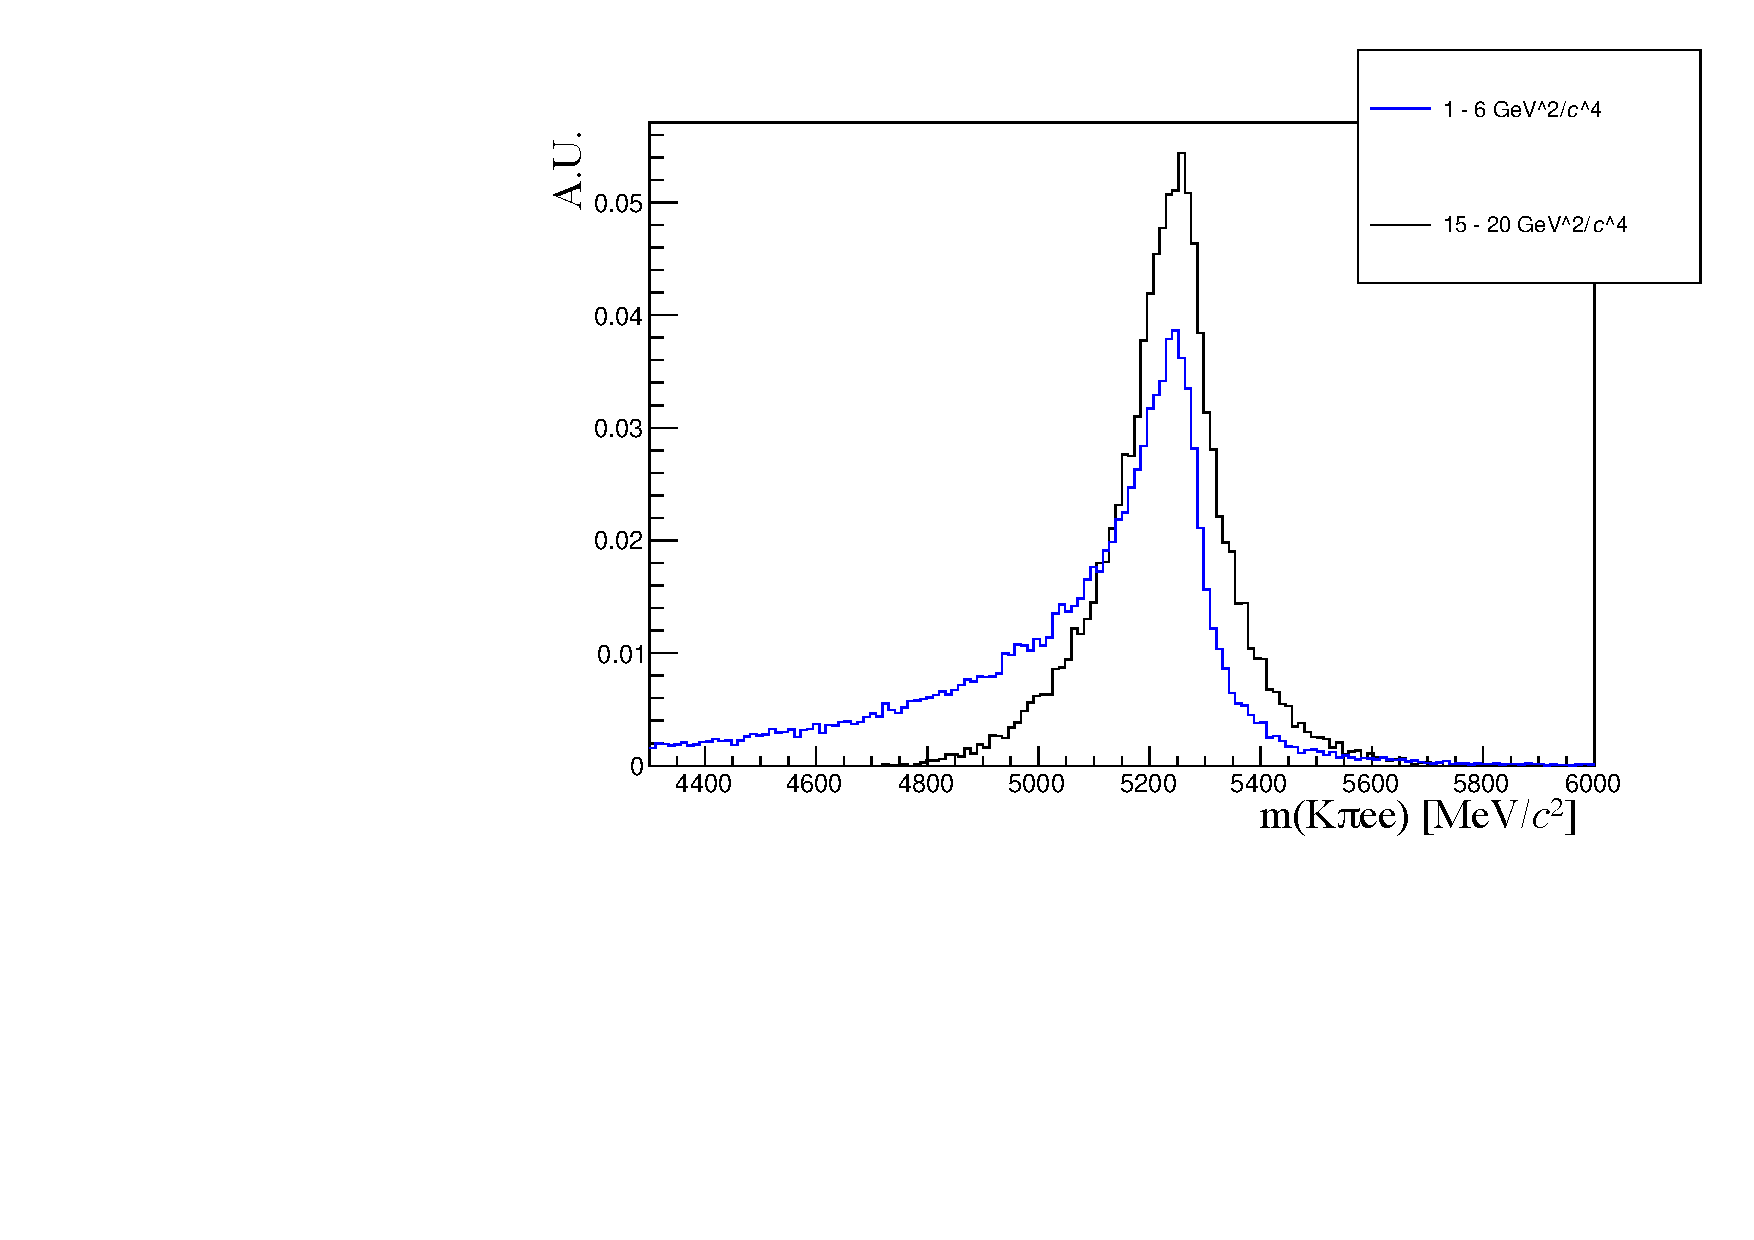
\includegraphics[width=0.70\textwidth]{RKst/figs/high_central_mass_comparison.pdf}
\caption{Simulated m($K\pi ee$) invariant mass in the $[1.1,6]$ and $[15,20]$~\gevgevcccc~\qsq intervals.  }
\label{fig:high_central_mass_comparison}
\end{figure}

The distribution of the \mKpiee mass in the $0\gamma$ category is characterised by a sharp tail on the righthand side and is described 
with a Crystal Ball function (CB), while the $1\gamma$ and $2\gamma$ categories are modelled using the sum of a Crystal Ball 
and a Gaussian function (CBG) with independent parameters. In all the bremsstrahlung categories the distribution of the 4-body 
invariant mass with the \jpsi mass constraint, $m(K\pi ee)_{\jpsi}$, is modelled using the sum of a DCB and a Gaussian 
functions as done for the muon fit.
%
%All parameters obtained using simulation are fixed in the fit to data.
To account for possible data-simulation discrepancies, the mass (widths) of each trigger PDF is allowed to shift (scale), similarly to the muon channels.
However, due to the larger background contamination these parameters are shared between the rare and the \BdToKstJPsee control sample.
%The tail parameters are similar between the $\jpsi(ee)$ and the central-\qsq but this is not the case at high-\qsq, as can be seen
%in Fig.~\ref{fig:high_central_mass_comparison}, due to the migration of candidates in the tail to lower reconstructed \qsq.
%For this reason the initial parameters for each candidate type are obtained fitting a simulated sample of the same candidate type. 

%Finally, combining the three bremsstrahlung PDFs one needs to specify in which fractions they contribute to the total.

The $f^{L0}_{n\gamma}$ fractions have been shown to be in good agreement between 
resonant data and simulation and therefore they are fixed to the simulated values, separately
for the normalisation channel and each \qsq interval. Table~\ref{tab:brem_frac} lists the percentages
of candidates with 0, 1 and 2 recovered photons for each trigger category.

In summary the signal PDF for the fit on data is defined as:
%
\begin{equation}
\begin{array} {ll}
\mathcal{P}_{sig}(m;c,m') & = \sum\limits_{L0}^{} \;[ \, f^{\rm L0}_{0\gamma} \cdot \mathcal{P}^{\rm L0}_{0\gamma}(m;c,m')  \\
& + \, f^{\rm L0}_{1\gamma} \cdot \mathcal{P}^{\rm L0}_{1\gamma}(m;c,m') + (1 - f^{\rm L0}_{0\gamma} - f^{\rm L0}_{1\gamma}) \cdot \mathcal{P}^{\rm L0}_{2\gamma}(m;c,m')]
\end{array} 
\end{equation}
%
where the free parameters are: $c$, the widths' scaling factor, and $m'$, the mass shift.


\subsubsection{Background PDFs for the electron channels}
\label{sec:RKst_misreco_fit}

This section reports the background components considered for each fitted sample.

\subsubsection*{\BdToKstee low-\qsq}

\begin{itemize}

\item \textit{Combinatorial}: described using an exponential function; the yield and slope parameters are free to vary in the fit;

\item \textit{Partially-reconstructed} (hadronic): the shape is obtained from a $K_1^+(1270)$ simulated samples smoothed with
a \verb!RooKeysPdf!. Simulated distributions are shown in Fig.~\ref{fig:misreco}. The fraction of partially-reconstructed 
candidates with respect to signal ones is expected to be very similar to that
in \BdToKstGee and therefore the normalisation is fixed as:
%
$$N_{\ee, \, {\rm low}}^{\rm part-reco} = N_{\ee} \cdot \frac{N_{\gamma(ee)}^{\rm part-reco}}{N_{\gamma(ee)}},$$
%
where $N_{\gamma(ee)}^{\rm part-reco (hadronic)}/N_{\gamma(ee)}$ is the fraction of hadronic partially-reconstructed background candidates relative to the signal yield in the \BdToKstGee channel;

\item \textit{\BdToKstG leakage}: the leakage from the \BdToKstGee decay into the low-\qsq region is modelled using simulated candidates that pass the low-\qsq requirements: the distribution is smoothed using a \verb!RooKeysPdf!; the normalisation is fixed to the \BdToKstGee yield, $N_{\gamma(ee)}$ as:
%
$$N_{\ee, \, {\rm low}}^{\rm leak} = N_{\gamma(ee)} \cdot f_{\gamma(ee)}^{\rm leak, \,MC},$$
%
where $f_{\gamma(ee)}^{\rm leak, \,MC}$ is the fraction of $\gamma(ee)$ simulated candidates which leaks in the low-\qsq region.

\end{itemize}


\subsubsection*{\BdToKstee central-\qsq}

\begin{itemize}

\item \textit{Combinatorial}: described using an exponential function;
the yield and slope parameters are free to vary in the fit.

\item \textit{Partially-reconstructed} (hadronic): modelled using simulation as described for the low-\qsq 
but in this case the normalisation is left free to vary.

%fixed with respect to the signal yield, $N_{\ee}$, as:
%
%$$N_{\ee}^{\rm mis-reco} = N_{\ee} \cdot \frac{N_{\jpsi(ee)}^{\rm mis-reco (hadronic)}}{N_{\jpsi(ee)}},$$
%
%where $N_{\jpsi(ee)}^{\rm mis-reco (hadronic)}/N_{\jpsi(ee)}$ is the fraction of hadronic mis-reconstructed background relative
%to the signal yield in the $\Bd\to\Kstarz(\jpsi\to\ee)$ channel. Note that the leptonic mis-reconstructed background is not modelled
%because it does not contribute in the rare samples.

\item \textit{\BdToKstJPs leakage}: the leakage from the \jpsi radiative tail into the central-\qsq interval is modelled by selecting 
simulated \BdToKstJPsee candidates which pass the central-\qsq requirements and smoothing the distributions
with a kernel density estimation method. The normalisation is fixed to the $\Bs\to\Kstarz(\jpsi\to\ee)$ yield, 
$N_{\jpsi ee}$, as:
%
$$N_{\ee, \, {\rm central}}^{\rm leak} = N_{\jpsi(ee)} \cdot f_{\jpsi(ee)}^{\rm leak, \,MC},$$
%\frac{N_{\jpsi(ee)}^{\rm leak, \,MC}}{N_{\jpsi(ee)}^{\rm MC}},$$
%
%where $N_{\jpsi ee}^{\rm MC}$ is the number of \jpsi(ee) simulated events reconstructed in the \jpsi mass window (6--11\gevgevcccc), and $N_{\jpsi ee}^{\rm leak, \,MC}$ is the number of $\Bs\to\Kstarz(\jpsi\to\ee)$ simulated events leaking in the central-\qsq region.
where $f_{\jpsi(ee)}^{\rm leak, \,MC}$ is the fraction of $\Bd\to\Kstarz(\jpsi\to\ee)$ simulated candidates reconstructed
in the central-\qsq interval.

\end{itemize}

\subsubsection*{\BdToKstee high-\qsq}
%
\begin{itemize}

\item \textit{Combinatorial}: modelled using a shape obtained by reversing the neural network requirement on data,
which has the effect of selecting background candidates instead of signal ones.
Figure~\ref{fig:highq2_comb} shows the invariant mass distributions for different anti-cuts on the electron 
and muon samples at high-\qsq. The shapes are very similar between the two samples and as a function 
of the cut value. In order to have a larger statistics, the shape is taken from the muon sample with a tight
anti-MVA cut, $\verb!NNout! < 0.1$, and smoothed with a \texttt{RooKeysPdf};

\item \textit{Partially-reconstructed} (hadronic): modelled using simulation as described for the previous intervals;
 the normalisation is left free to vary.

\item \textit{\BdToKstPsi leakage}: the leakage from the \psitwos radiative tail is modelled using simulated 
\BdToKstPsiee candidates which pass the the high-\qsq requirements. The normalisation is fixed to 
the $\psitwos(ee)$ yield, $N_{\psitwos(ee)}$ as:
%
$$N_{\ee, \, {\rm high}}^{\rm leak} = N_{\psitwos(ee)} \cdot f_{\psitwos(ee)}^{\rm leak, \,MC},$$
%
where $f_{\psitwos(ee)}^{\rm leak, \,MC}$ is the fraction of $\Bd\to\Kstarz(\psitwos\to\ee)$ simulated candidates
leaking into the high-\qsq interval.

\end{itemize}

\subsubsection*{\BdToKstG}

\begin{itemize}

\item \textit{Combinatorial}: described using an exponential function; the yield and slope parameters are free to vary in the fit;

\item \textit{Partially-reconstructed} (hadronic): modelled using simulation as described for the previous intervals;
 the normalisation is left free to vary and used to constrain the fraction of partially-reconstructed candidates in the low-\qsq interval.

\item \textit{\BdToKstee leakage}: as the $\Kstarz\gamma$ was added to the low-\qsq also the low-\qsq leakage is added
to $\Kstar\gamma$. The yield is constrained to the $N_{ee}^{low}$ yield.

\end{itemize}

\begin{figure}[t!]
\centering
%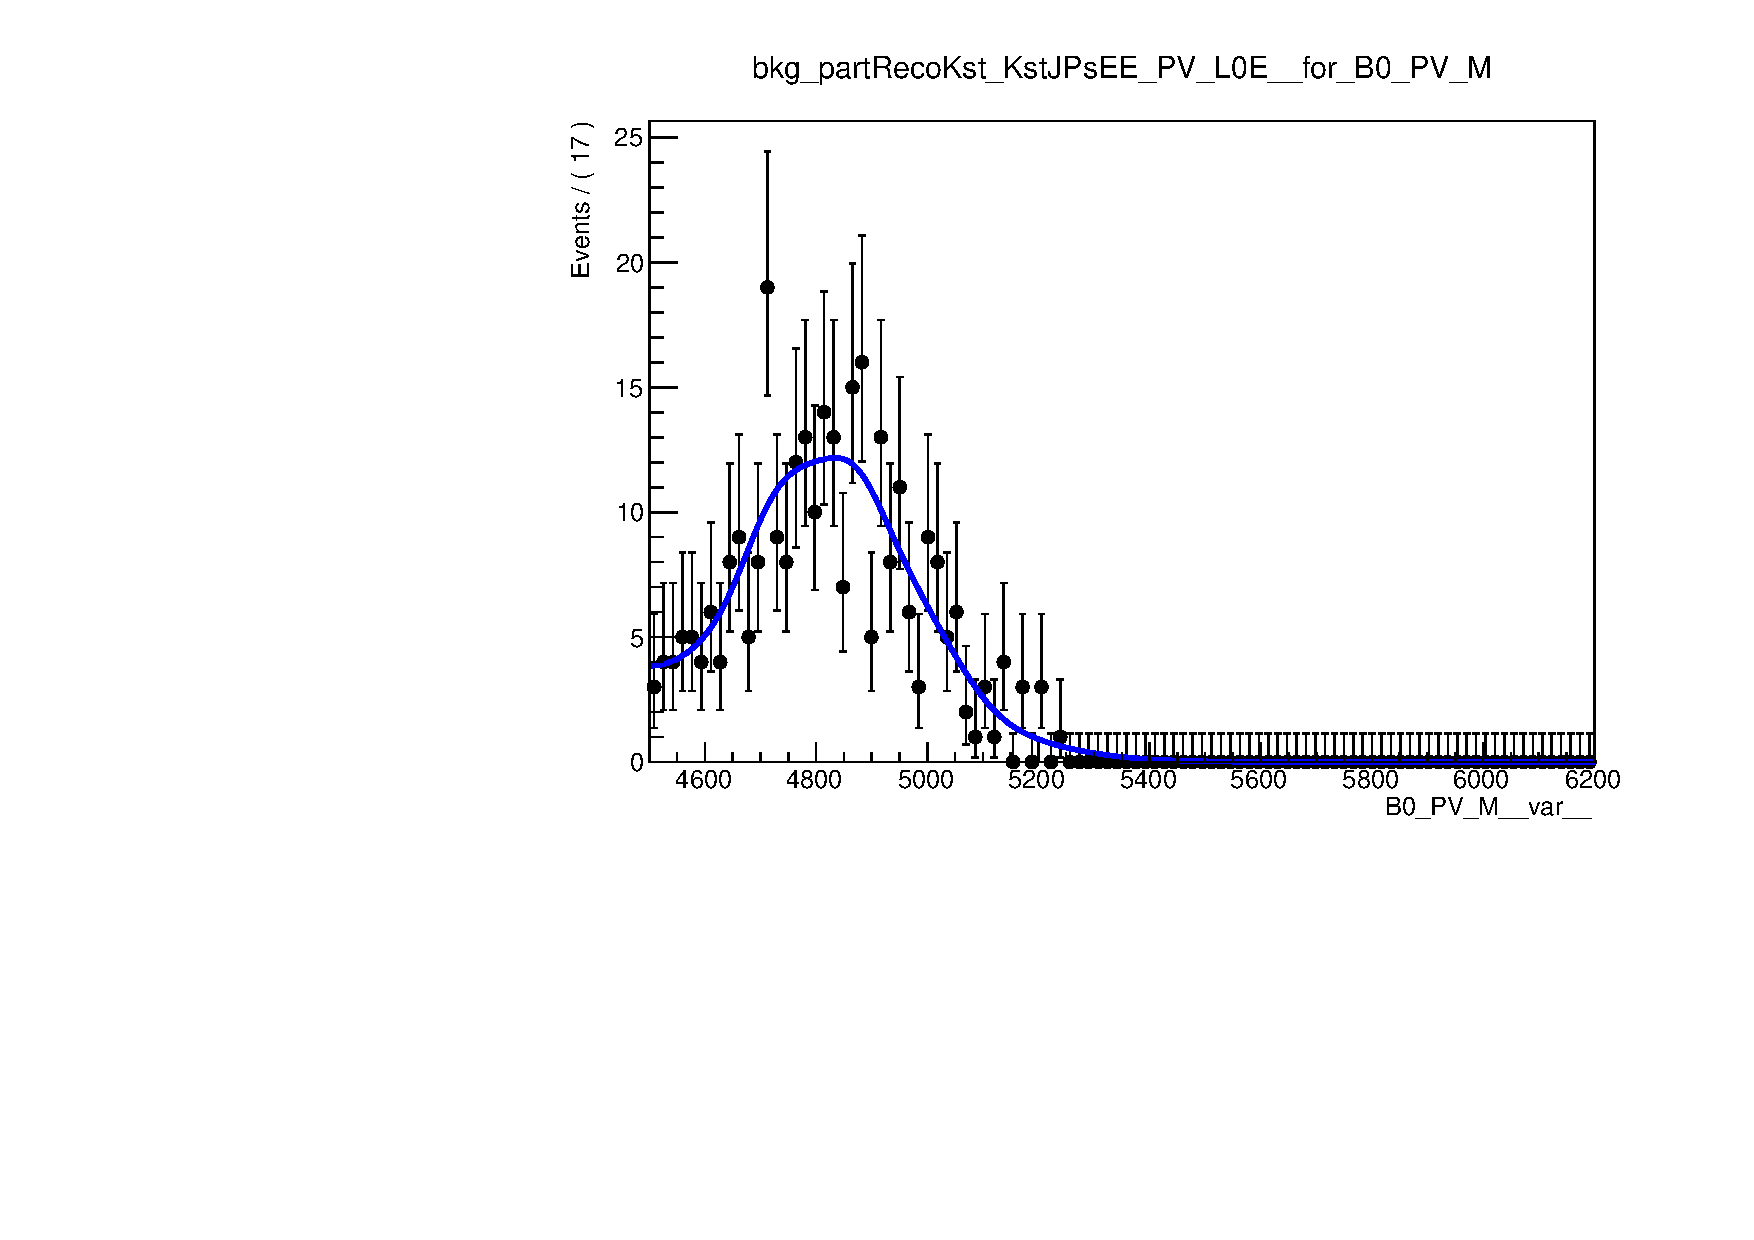
\includegraphics[width=0.49\textwidth]{RKst/figs/Fit/fit_EE/rooKeysModel_bkg_partRecoKst_KstJPsEE_PV_L0E__for_B0_PV_M.pdf}
%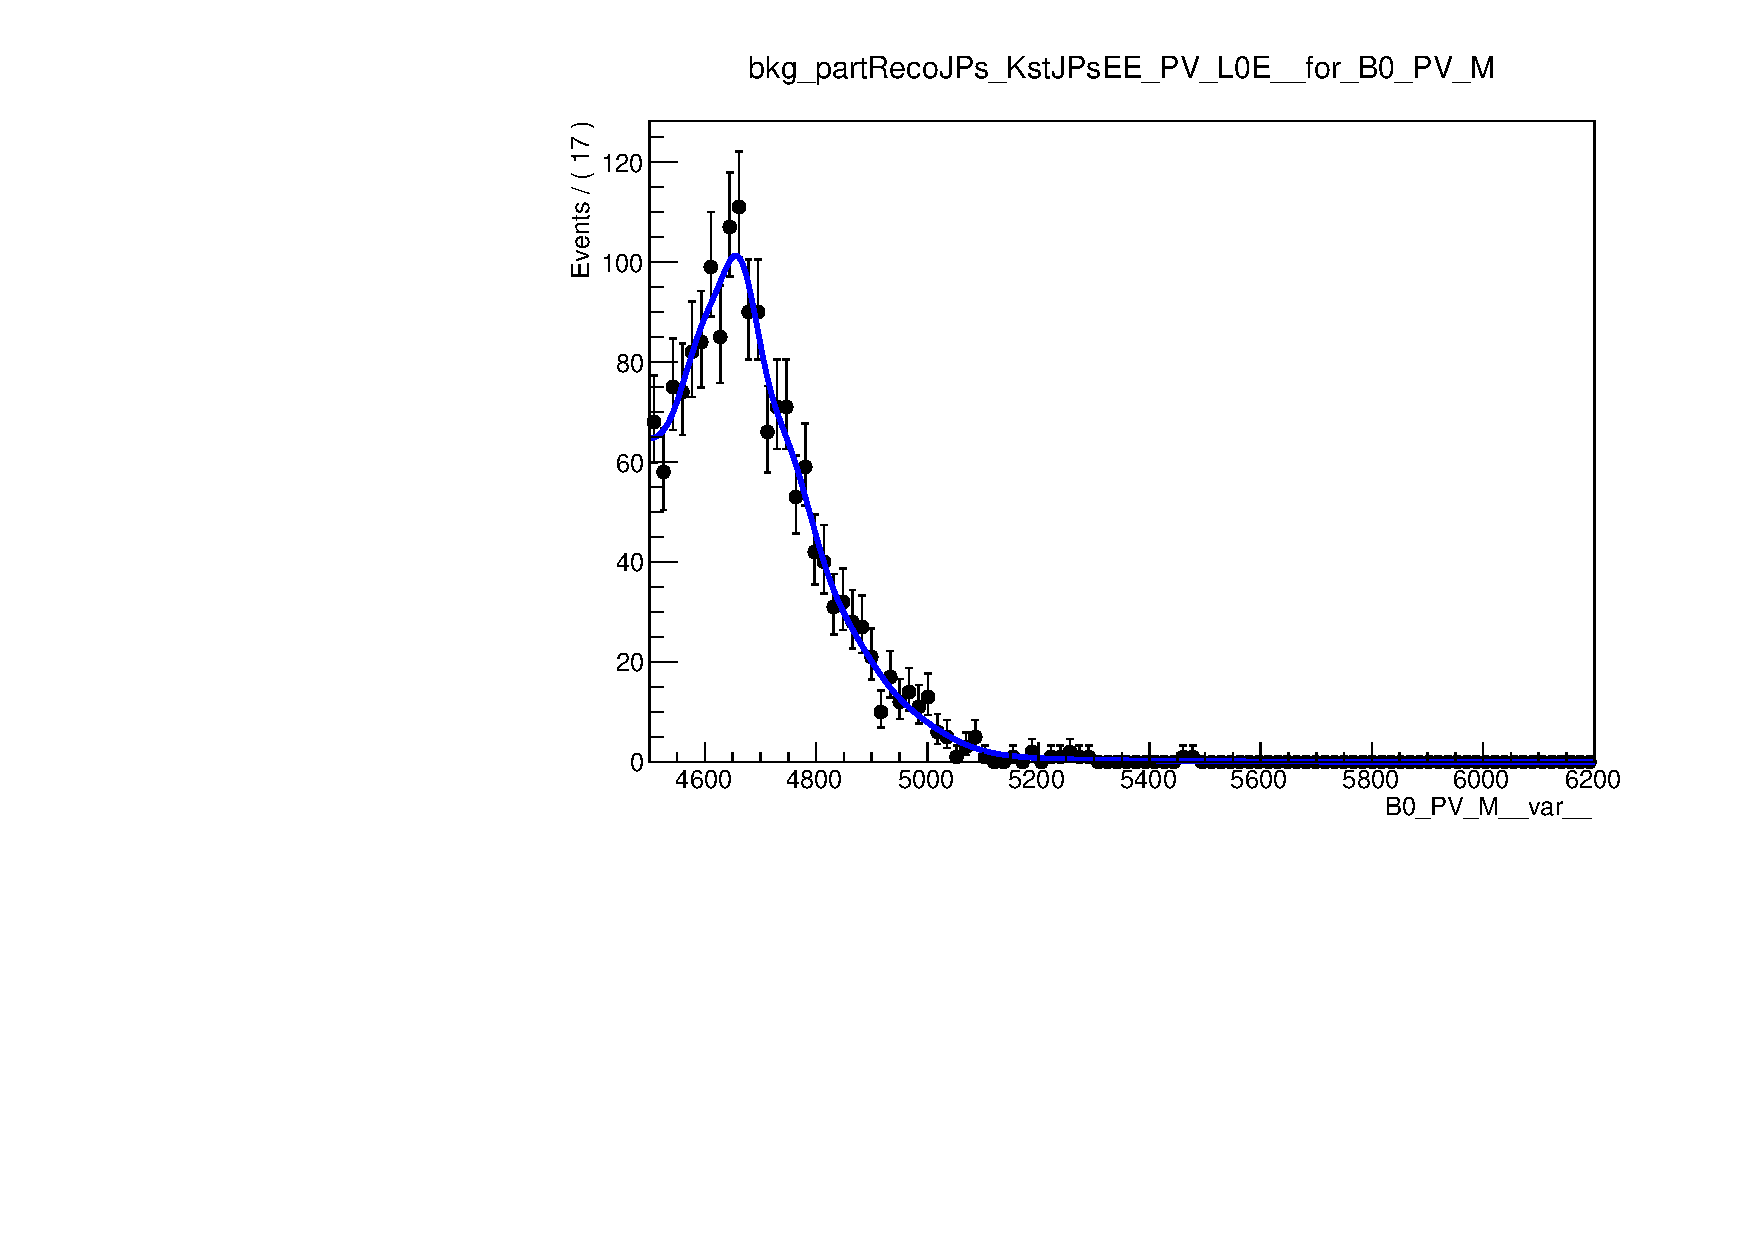
\includegraphics[width=0.49\textwidth]{RKst/figs/Fit/fit_EE/rooKeysModel_bkg_partRecoJPs_KstJPsEE_PV_L0E__for_B0_PV_M.pdf}
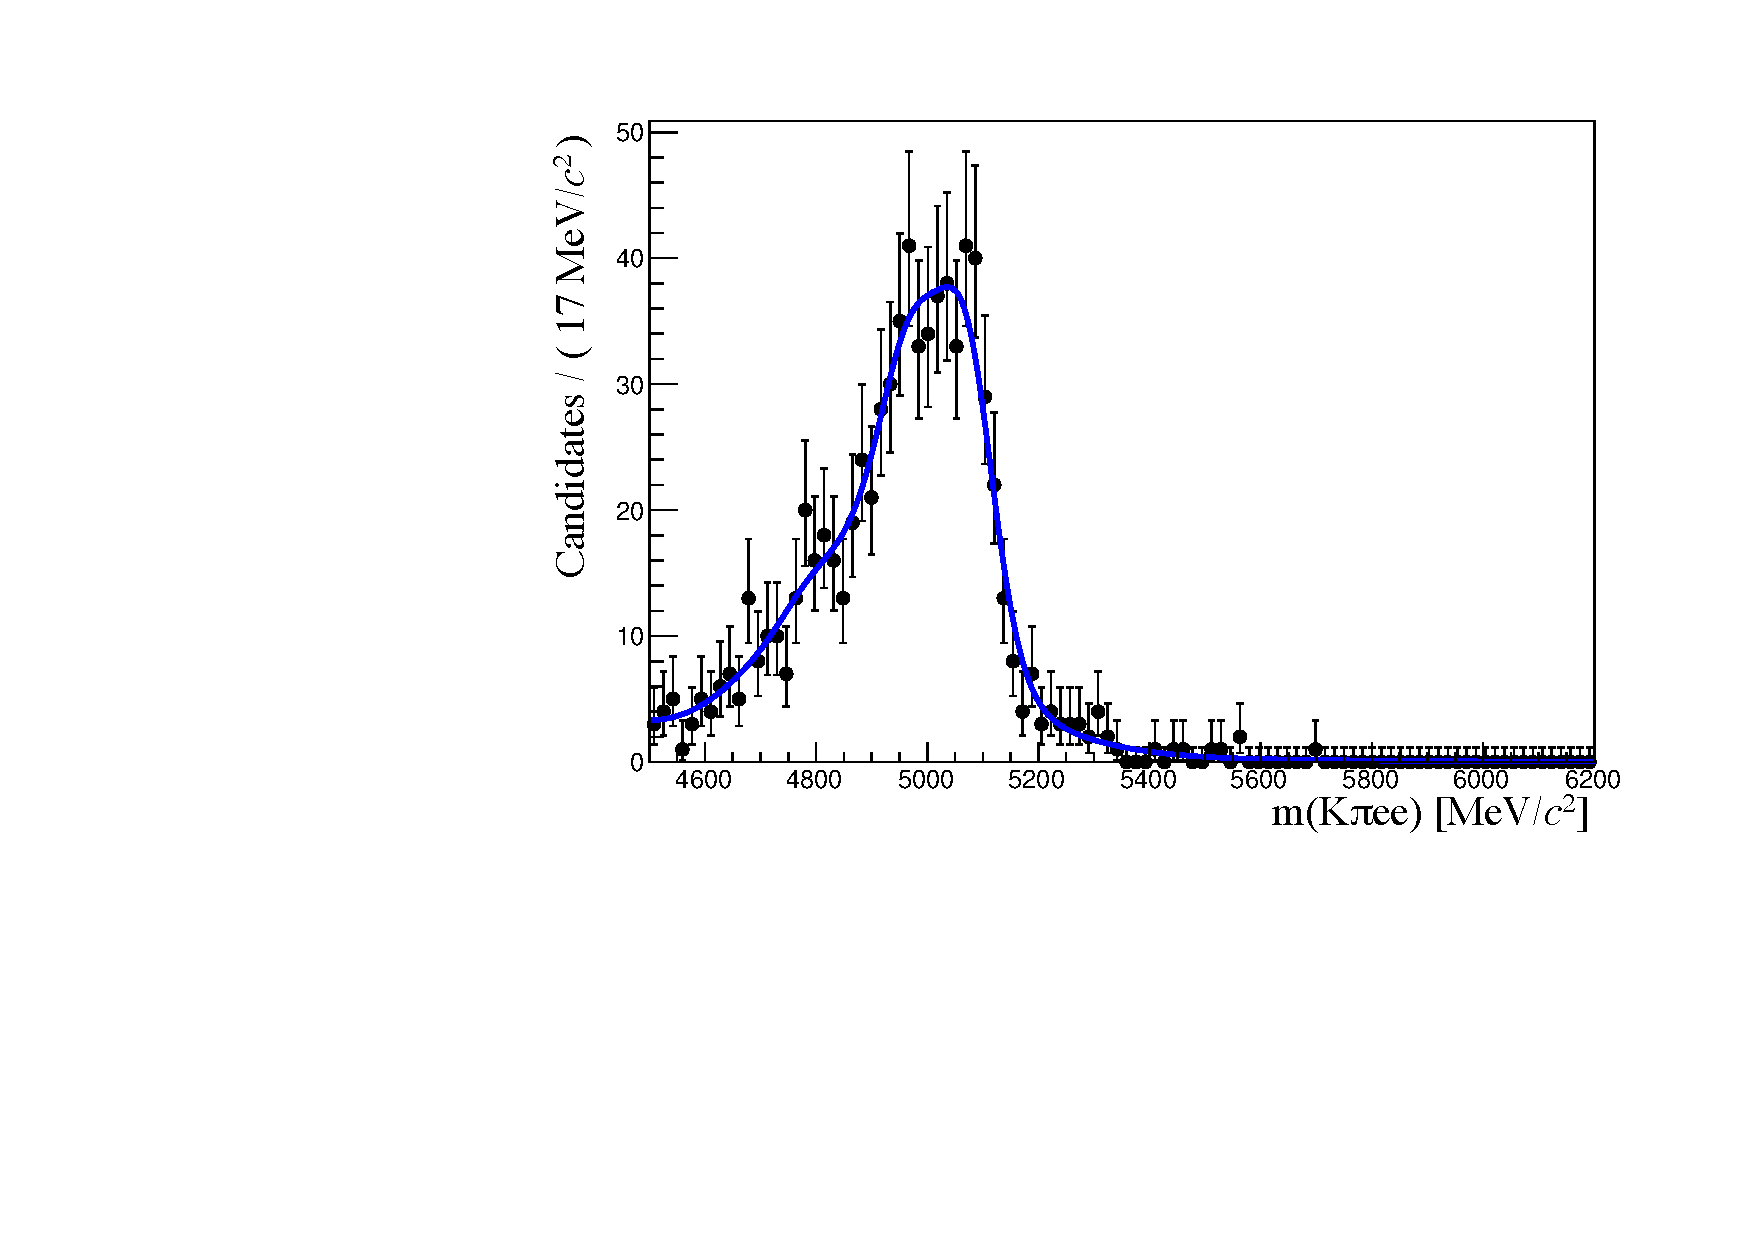
\includegraphics[width=0.49\textwidth]{RKst/figs/Fit/fit_EE/rooKeysModel_bkg_partReco_KstEE_low_L0E__for_B0_PV_M.pdf}
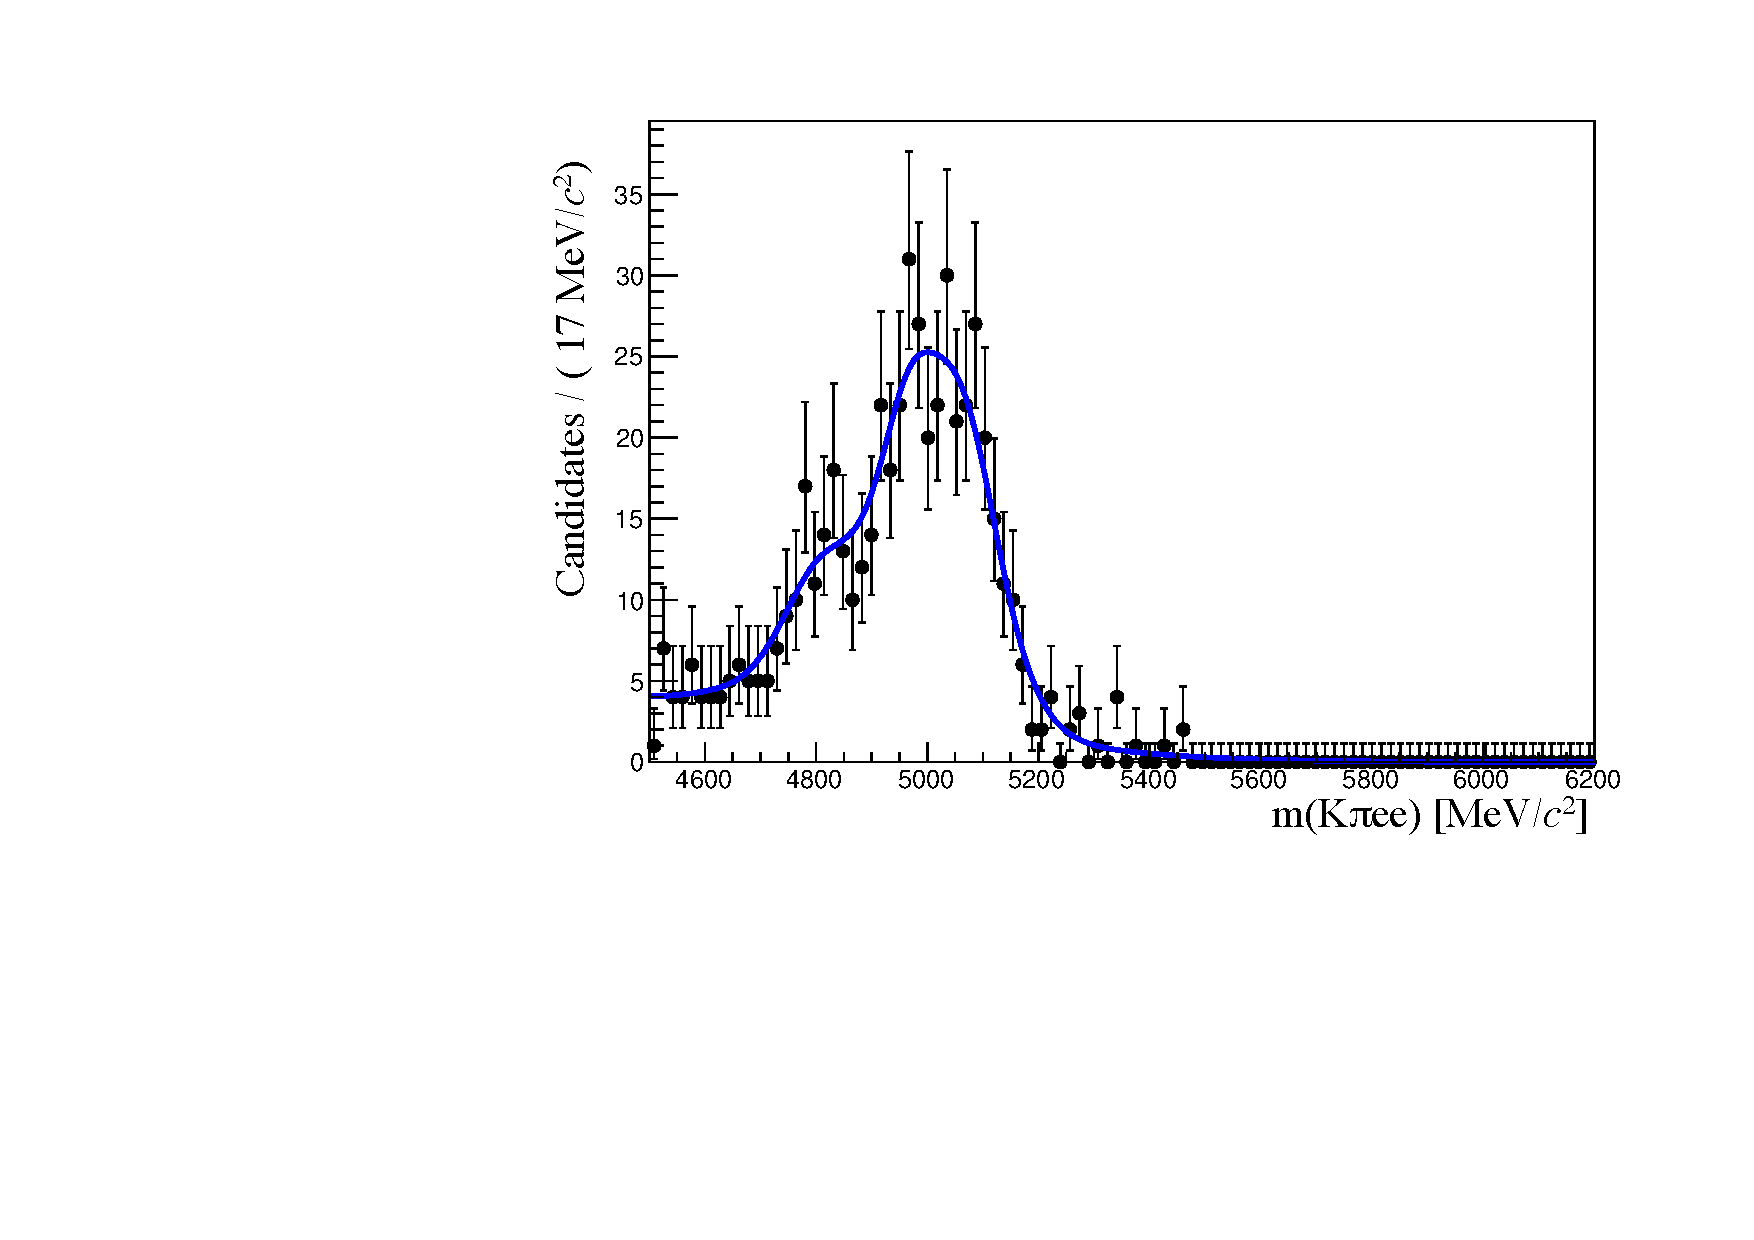
\includegraphics[width=0.49\textwidth]{RKst/figs/Fit/fit_EE/rooKeysModel_bkg_partReco_KstEE_central_L0E__for_B0_PV_M.pdf}
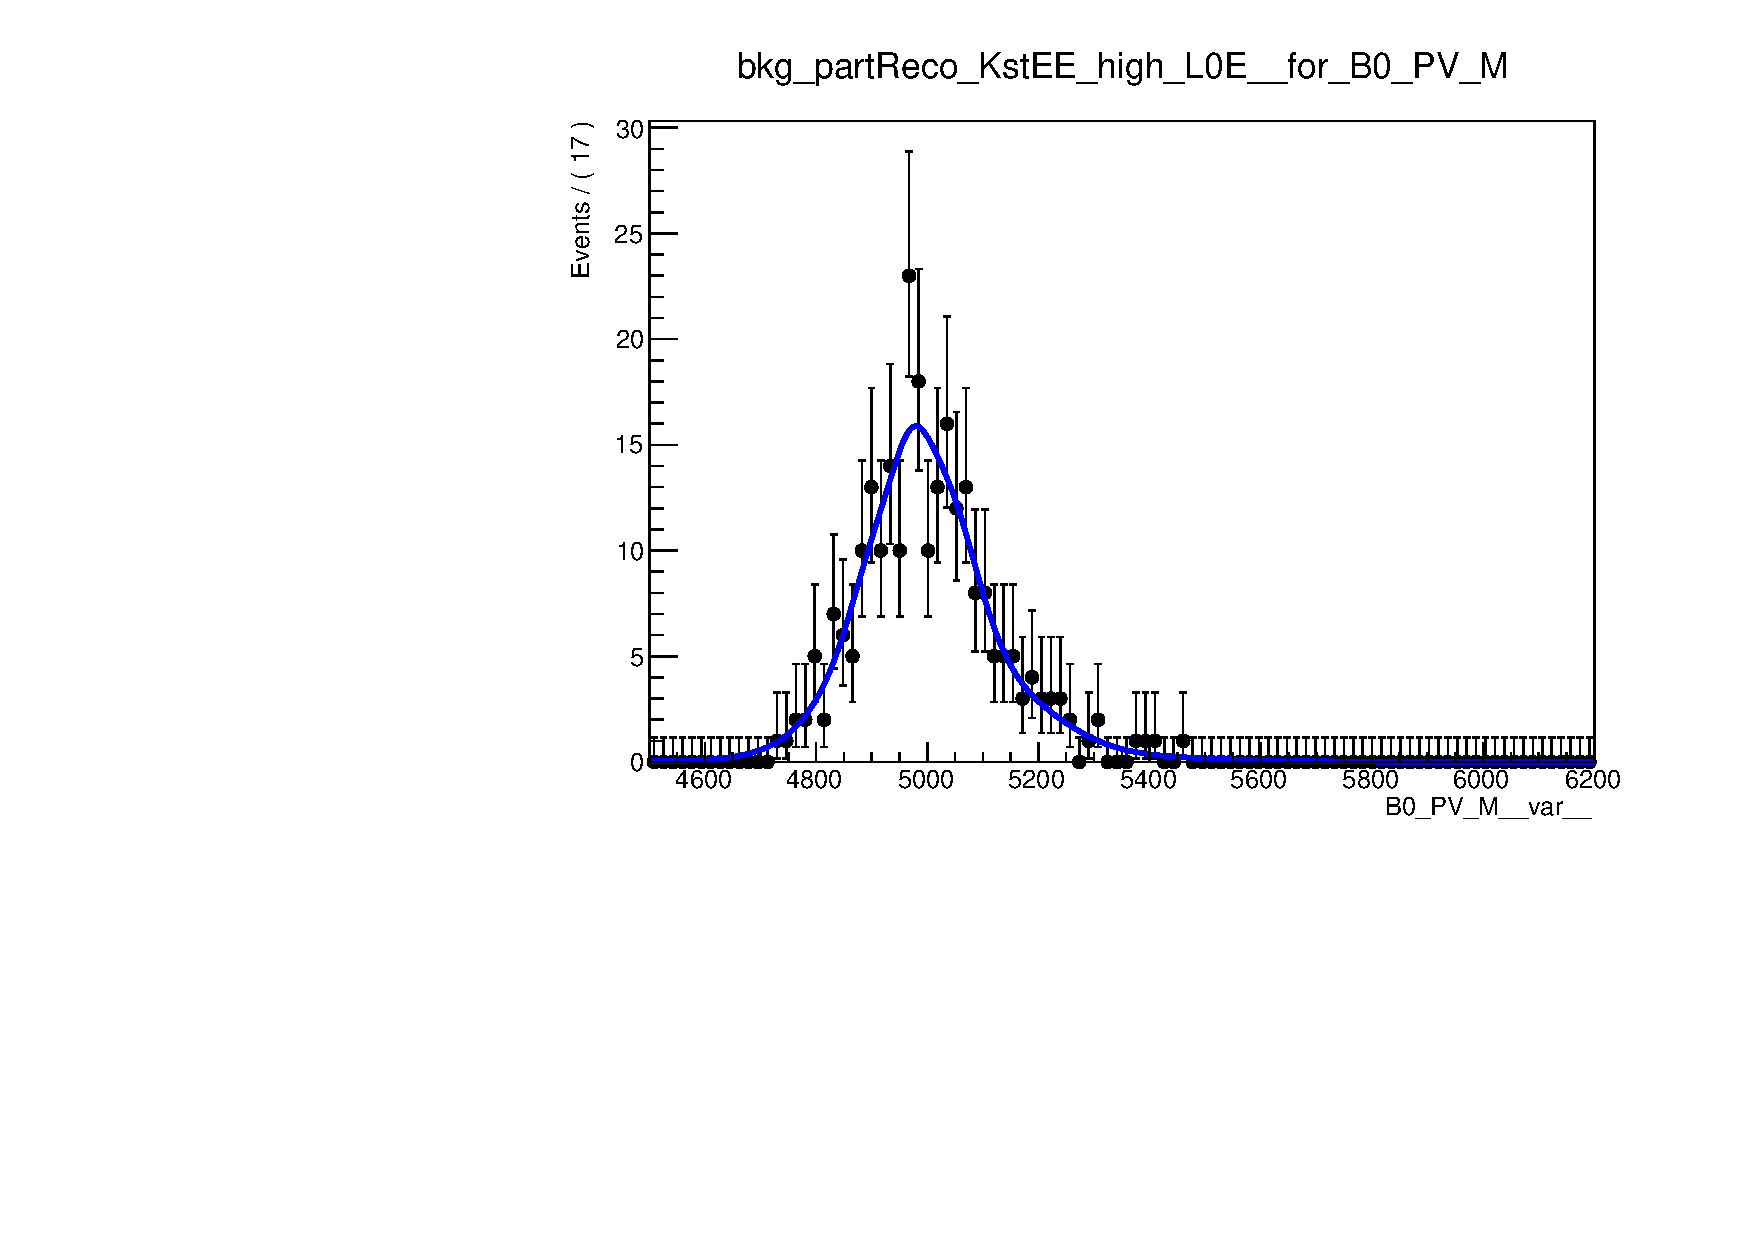
\includegraphics[width=0.49\textwidth]{RKst/figs/Fit/fit_EE/rooKeysModel_bkg_partReco_KstEE_high_L0E__for_B0_PV_M.pdf}
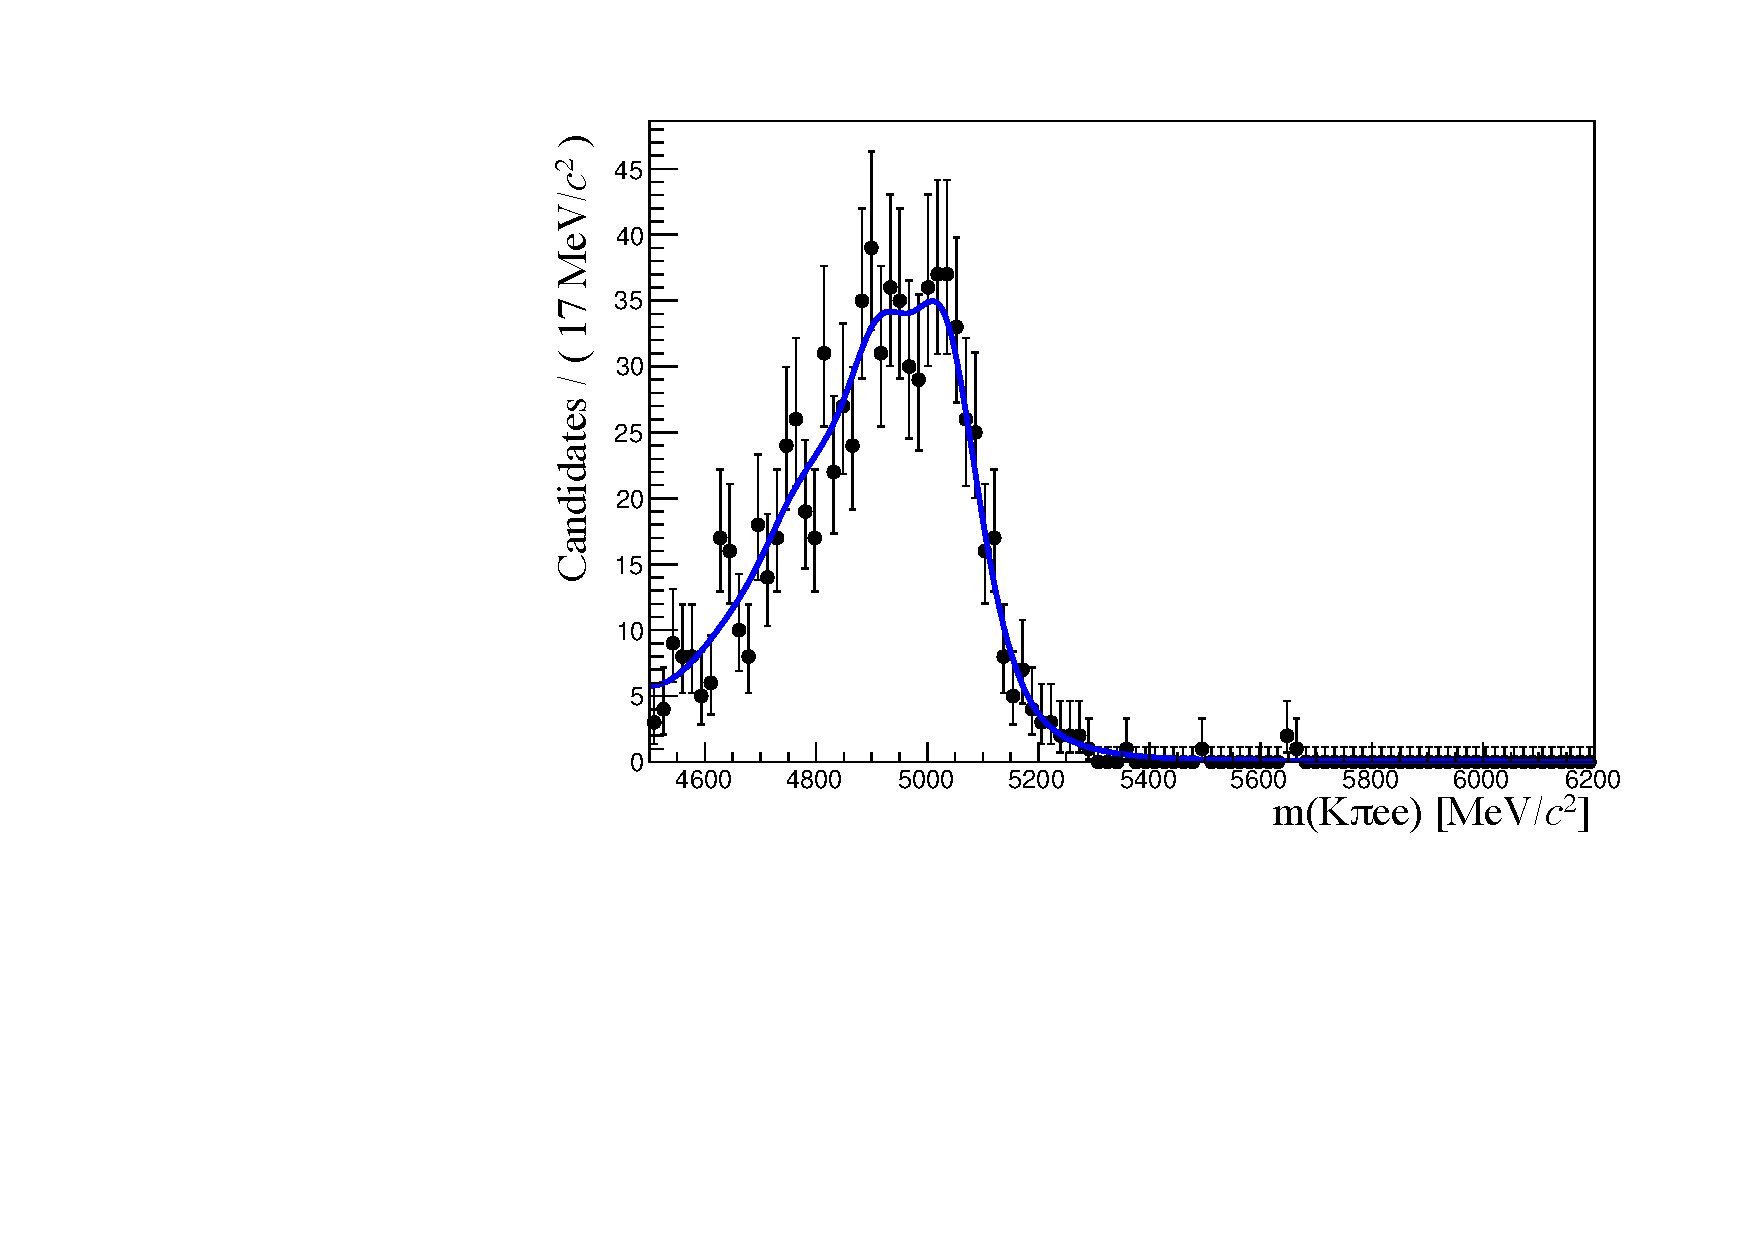
\includegraphics[width=0.49\textwidth]{RKst/figs/Fit/fit_EE/rooKeysModel_bkg_partReco_KstGEE_L0E__for_B0_PV_M.pdf}
\caption{Distributions of the \mKpiee invariant mass of decays involving
higher \Kstarz resonances for the (top left) low- (top right) central-, (bottom left) high-\qsq intervals 
and (bottom right) \BdToKstGee.}
\label{fig:misreco}
%\end{figure}

\vspace{2cm}

%\begin{figure}[t!]
\centering
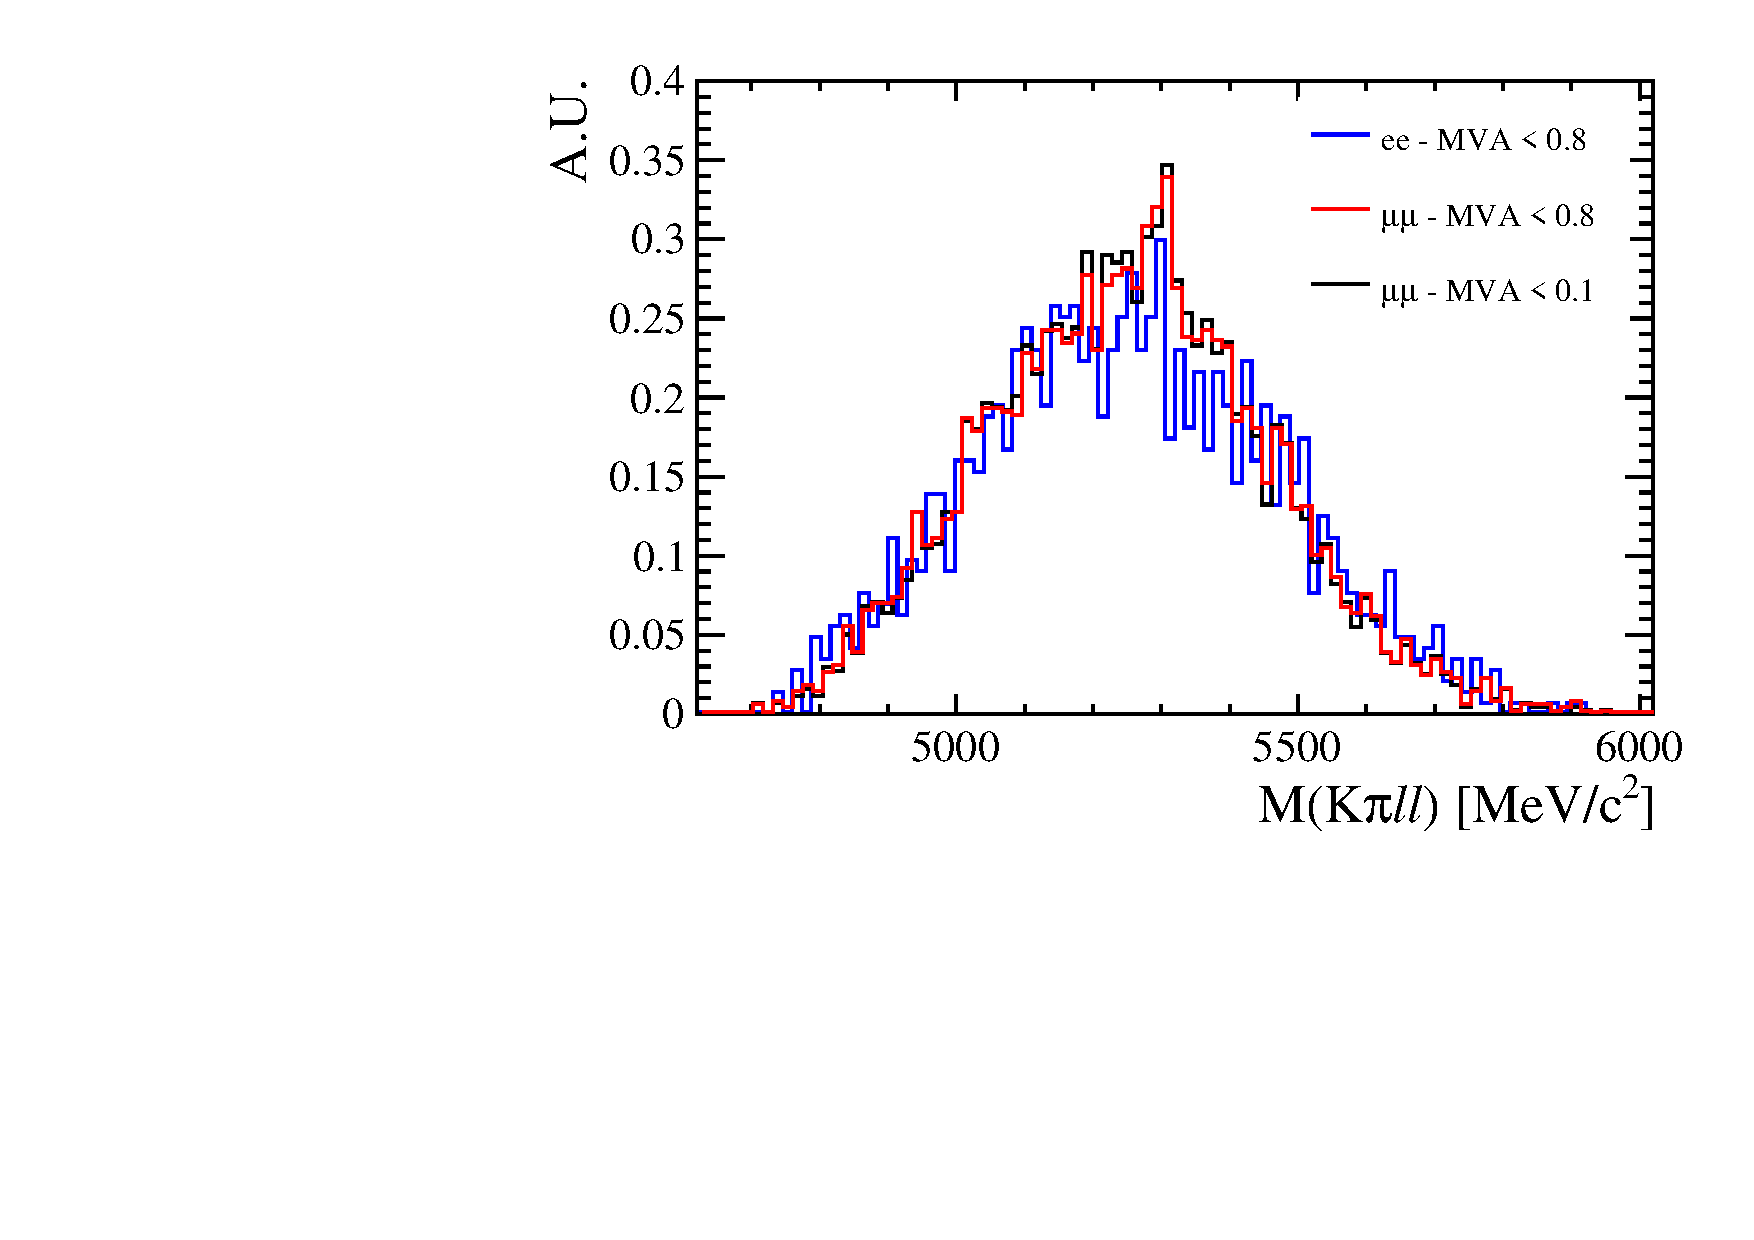
\includegraphics[width=0.7\textwidth]{RKst/figs/Background/highq2_comb.pdf}
\caption{Distributions of the \mKpill invariant mass for \BdToKstll candidates selected with a reversed cut on the neural network output.}
\label{fig:highq2_comb}
\end{figure}

\subsubsection*{\BdToKstJPs and \BdToKstPsi}

The following backgrounds are considered for the fits to the invariant mass of \BdToKstJPsee candidates:
%
\begin{itemize}

\item \textit{Combinatorial}: described using an exponential function. The yield and slope parameters are free to vary in the fit;

\item $\Lb\to pK(\jpsi\to\ee)$: described using simulated candidates to which the full selection is applied. This distribution has a broad 
shape under the signal peak and is smoothed using a \texttt{RooKeysPdf}. The normalisation is constrained to the 
$\Lb\to pK(\jpsi\to\mumu)$ yield returned by the muon fit after correcting for efficiency differences between final states with muons and electrons.

\item $\Bs\to\Kstarz(\jpsi\to\ee)$: described using the same PDF adopted for the signal, but a different central value, $m_0$, which is set at the \Bs nominal mass. The normalisation is constrained to the $\Bd\to\Kstarz(\jpsi\to\mumu)$ yield returned by the muon fit after correcting for efficiency differences between final states with muons and electrons;

\end{itemize}

The \jpsi mass constraint has the effect of pushing the partially-reconstructed background away from 
the peak outside the fit window. The \jpsi control sample is selected using the requirement that the 4-body 
mass constrained using \verb!DecaTreeFitter! is above 5150~\mevc, which explicitly removes
the partially-reconstructed background; this cut does not produce significant distortion to the
unconstrained invariant mass distribution in the considered window. 
For these reasons this background does not need to be modelled in either of these cases.
%
%, used as control sample, includes further components:
%
%\begin{itemize}
%
%\item \textit{Partially-reconstructed}: the partially-reconstructed background from both higher hadronic and \ccbar resonances
%is modelled using inclusive \decay{\Bz}{\jpsi X} simulated events to which the full selection is applied. The invariant mass distributions 
%of these candidates, shown in Fig.~\ref{fig:misreco}, is smoothed using a kernel estimation method and the yield is left free to vary;
%
%. Given the little statistics available, the same shape 
%is used for all the trigger categories
%
%events to which the full selection is applied
%this background is split in an hadronic component, involving higher hadronic resonances, 
%and a leptonic one, coming from higher \ccbar resonances. Both categories are modelled using inclusive \decay{\Bz}{\jpsi X} simulated 
%events to which the full selection is applied. The distribution for the hadronic (leptonic) category is defined by selecting candidates where 
%the \Kstarz (\jpsi) is not a direct daughter of the \Bz. The invariant mass distributions of these candidates, shown in Fig.~\ref{fig:misreco}, are 
%smoothed using a kernel estimation method and their yields are left free to vary in the fit. Given the little statistics available, the same shape 
%is used for all the trigger categories;
%
%\item \textit{\BdToKstPsi leakage}: the leakage from the \psitwos radiative tail into the \jpsi interval is modelled by 
%selecting simulated $\psitwos\to\ee$ which pass the requirements for \jpsi candidates. The normalisation is fixed 
%to the $\Bd\to\Kstarz(\psitwos\to\ee)$ yield, $N_{\psitwos(ee)}$, as:
%
%$$N_{\jpsi(ee)}^{\rm leak} = N_{\psitwos(ee)} \cdot f_{\psitwos(ee)}^{\rm leak, \,MC},$$
%\frac{N_{\psitwos(ee)}^{\rm leak, \,MC}}{N_{\psitwos(ee)}^{\rm MC}},$$
%
%where $f_{\psitwos(ee)}^{\rm leak, \,MC}$ is the fraction of $\Bd\to\Kstarz(\psitwos\to\ee)$ simulated events reconstructed in the \jpsi interval.
%
%\end{itemize}
%
For the fit to \BdToKstPsiee candidates, which includes a \psitwos mass constraint, only the combinatorial background is considered
and described using an exponential function.
%

%\clearpage

\subsubsection{Summary of the fit to the electron samples}

In summary, the free parameters in the fit to data are:
%
\begin{itemize}
\item the \BdToKstJPsee, \BdToKstPsiee and \BdToKstGee yields in each trigger category;
\item the $r_{ee}$ ratio common to all trigger categories; one for the low, one for the central- and one for the high-\qsq region;
\item one mass shift, $m'$, and one width scale factor, $c$, for the signal PDF common between \BdToKstJPsee and \BdToKstee in all intervals,
but different for the three trigger categories and for \BdToKstPsiee and \BdToKstGee;
\item the yield and slope, when applicable (e.g. no slope at high-\qsq), of the combinatorial background in each trigger category and for each channel;
\item the yield of the backgrounds when not fixed as described in the previous section.
\end{itemize}

Fits to simulated \BdToKstJPsee candidates are shown in Appendix~\ref{app:RKMCfits}, while
fits to real candidates are shown in Fig.~\ref{fig:fitJPsEE} for the normalisation channel, in Fig.~\ref{fig:fitsEE} 
for the rare channel and in Fig.~\ref{fig:fitsControlEE} for the control channels.
For simplicity the latter two figures show the sum of the three trigger categories, while the separate plots are
reported in Appendix~\ref{app:RKDatafits}, where fitted parameters are also reported on the plots.
%
In the high-\qsq interval, above 15~\gevgevcccc, the efficiency for the
L0Hadron trigger becomes very low as the \Kstarz has very low momentum.
In this region only 9 candidates are found spread in the interval
$4500 < m(K\pi ee) < 6000$ \mevcc. Therefore
only L0E and L0I triggered events are fitted for this region.

\subsection{Event yields}

Table~\ref{tab:RKst_yields} reports raw yields obtained from the
fits described in the previous subsections. The values for the rare channels and $\gamma(ee)$ are
 not parameters free to vary in the fits but, as described in Sec.~\ref{sec:rkst_fits}, they are parameterised
as a function of the number of resonant candidates found and the ratios $r_{ee}$ and $r_{\mu\mu}$
between the resonant and rare branching fractions; the values in the tables are derived from the ratios. 

%Measured values of these ratios are reported in Tab.~\ref{tab:RKst_results}.

%\clearpage

\begin{table}[t!]
\centering
\caption{Summary of the raw yields obtained from the invariant mass fits. The uncertainty is statistical.}
\label{tab:RKst_yields}
\renewcommand\arraystretch{1.4}
\begin{tabular}{$c|^c|^c|^c}
%\textbf{Sample} & \BdToKstGee & \BdToKstJPsll & \BdToKstPsiee \\ \hline
\rowstyle{\bfseries}
Sample & {\boldmath $\gamma(ee)$} & {\boldmath $\jpsi(ee)$} & {\boldmath $\psitwos(ee)$} \\ \hline
$\mu\mu$ 		& --	& $ 373755  \pm 641 $	& --  \\
$ee$ L0E 			& $ 614  \pm 35 $	& $ \phantom{0}42797  \pm 260 $	& $ 2701  \pm 62 $\\
$ee$ L0H 			& $ 262  \pm 24 $	& $ \phantom{00}3680  \pm 79\phantom{0} $		& $ \phantom{00}58  \pm 10 $\\
$ee$ L0I 			& $ 382  \pm 39 $	& $ \phantom{0}10804  \pm 138 $	& $ \phantom{0}569  \pm 32 $\\
\end{tabular}

\vspace{1cm}

\begin{tabular}{c|c|c|c}
%\rowstyle{\bfseries}
\textbf{Sample} & \textbf{low-}{\boldmath\qsq} & \textbf{central-}{\boldmath\qsq} & \textbf{high-}{\boldmath\qsq} \\ \hline
$\mu\mu$ 		& $ 475  \pm 24  $                 & $ 636  \pm 29  $ 			& $ 679  \pm 29 $  \\
$ee$ L0E 			& $ 117   \pm  12$         & $ 89   \pm  13$  & $ 158  \pm 26 $  \\
$ee$ L0H 			& $ \phantom{0}44   \pm  8\phantom{0}$         & $ \phantom{0}18   \pm  7\phantom{0}$ 	& 			-- 			 \\
$ee$ L0I 			& $ \phantom{0}72   \pm  11$        & $ \phantom{0}38   \pm  9\phantom{0}$ 	& $ \phantom{0}52  \pm 13 $  \\
\end{tabular}
\end{table}

%\begin{table}[t]
%\centering
%\caption{Raw yields of events found fitting invariant mass distributions of the rare and resonant events. }
%\renewcommand\arraystretch{1.25}
%\begin{tabular}{$c|^c^c^c}
%\rowstyle{\bfseries}
% Sample 			& 1.1--6~\boldmath{\gevgevcccc }			& 15--20~\boldmath{\gevgevcccc }		&\boldmath{ \jpsi}  \\ \hline
%$\mu\mu$ 		& $ \phantom{.}626  \pm 30\phantom{.}  $ 		& $ 605  \pm 27 $ 		& $ 333113  \pm 604 $ \\
%$ee$ L0E 			& $ \phantom{.}132   \pm  17\phantom{.}$   	& $ 137  \pm 27 $ 		& $ \phantom{x}48601  \pm 326 $ \\
%$ee$ L0H 			& $ 31.7   \pm  4.2$ 		& 			-- 						& $ \phantom{xx}4324  \pm 94\phantom{x} $ \\
%$ee$ L0I 			& $ 49.6   \pm  6.5$ 		& 			-- 						& $ \phantom{x}12791  \pm 172 $ \\
 %\end{tabular}
%\label{tab:RKst_yields}
%\end{table}

\begin{figure}[h!]
\centering
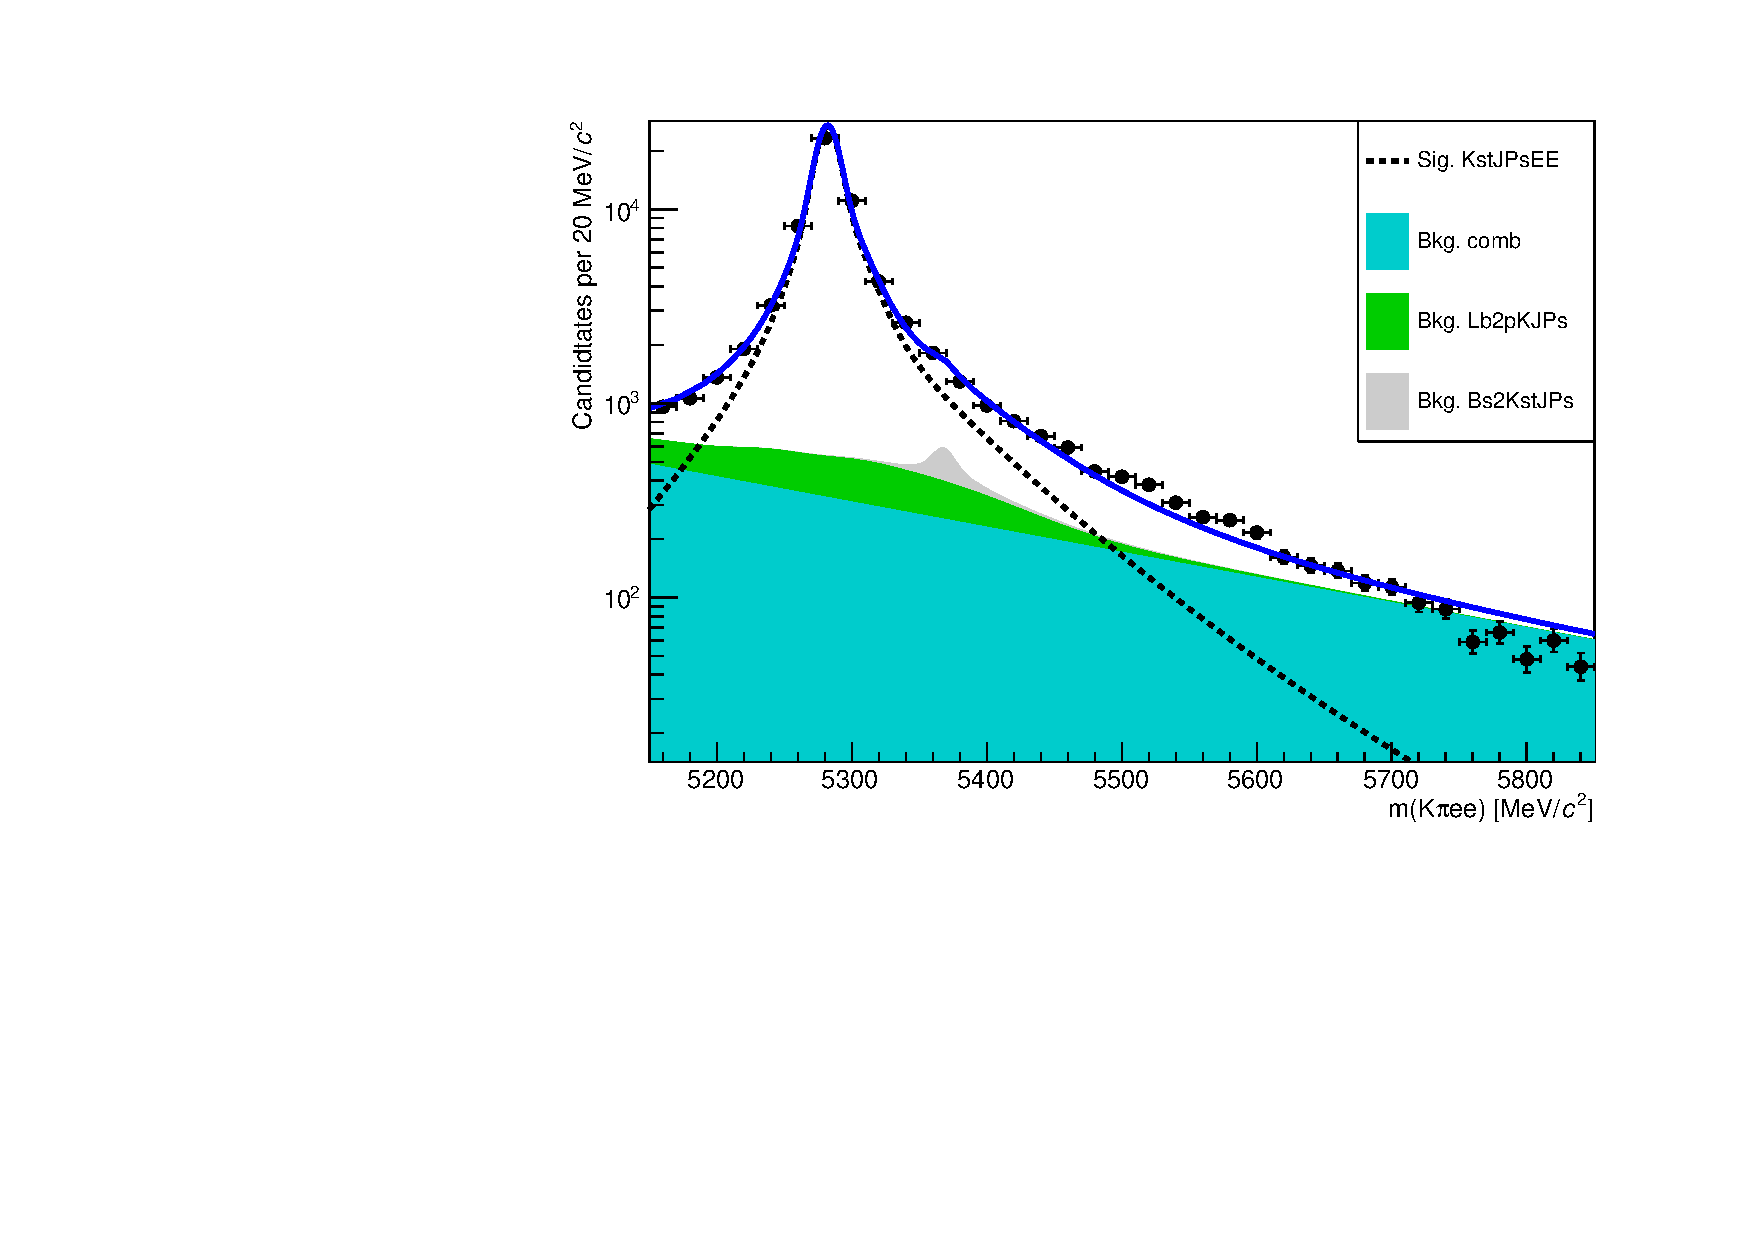
\includegraphics[width=0.7\textwidth]{RKst/figs/Fit/fit_EE/fit_JPs_L_log.pdf}
\caption{Fit to the mass constrained invariant mass, $\mKpiee_{\jpsi}$, of \BdToKstJPsee candidates.
The dashed black line represents the signal and the shaded shapes the backgrounds.}
\label{fig:fitJPsEE}
\end{figure}


\begin{figure}[h!]
\centering
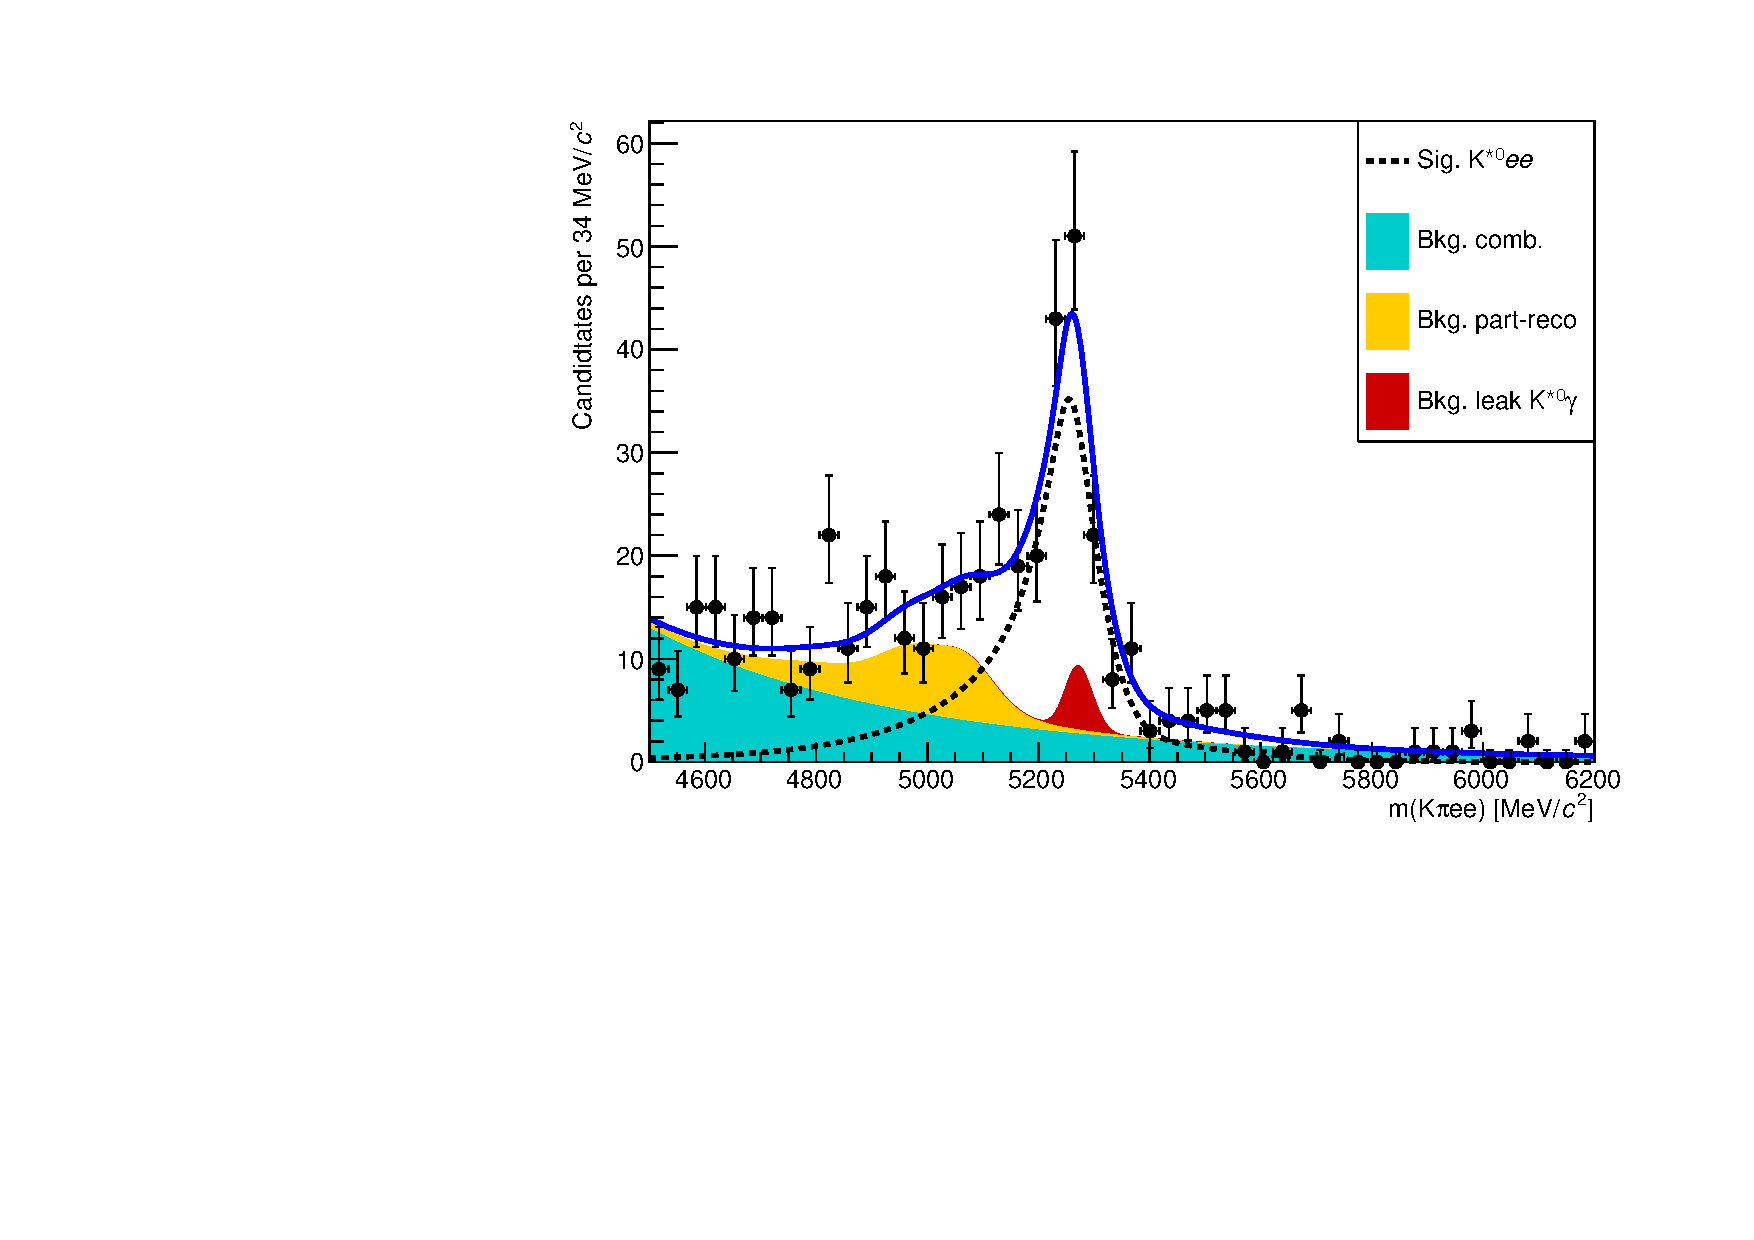
\includegraphics[width=0.7\textwidth]{RKst/figs/Fit/fit_EE/fit_EEl.pdf}
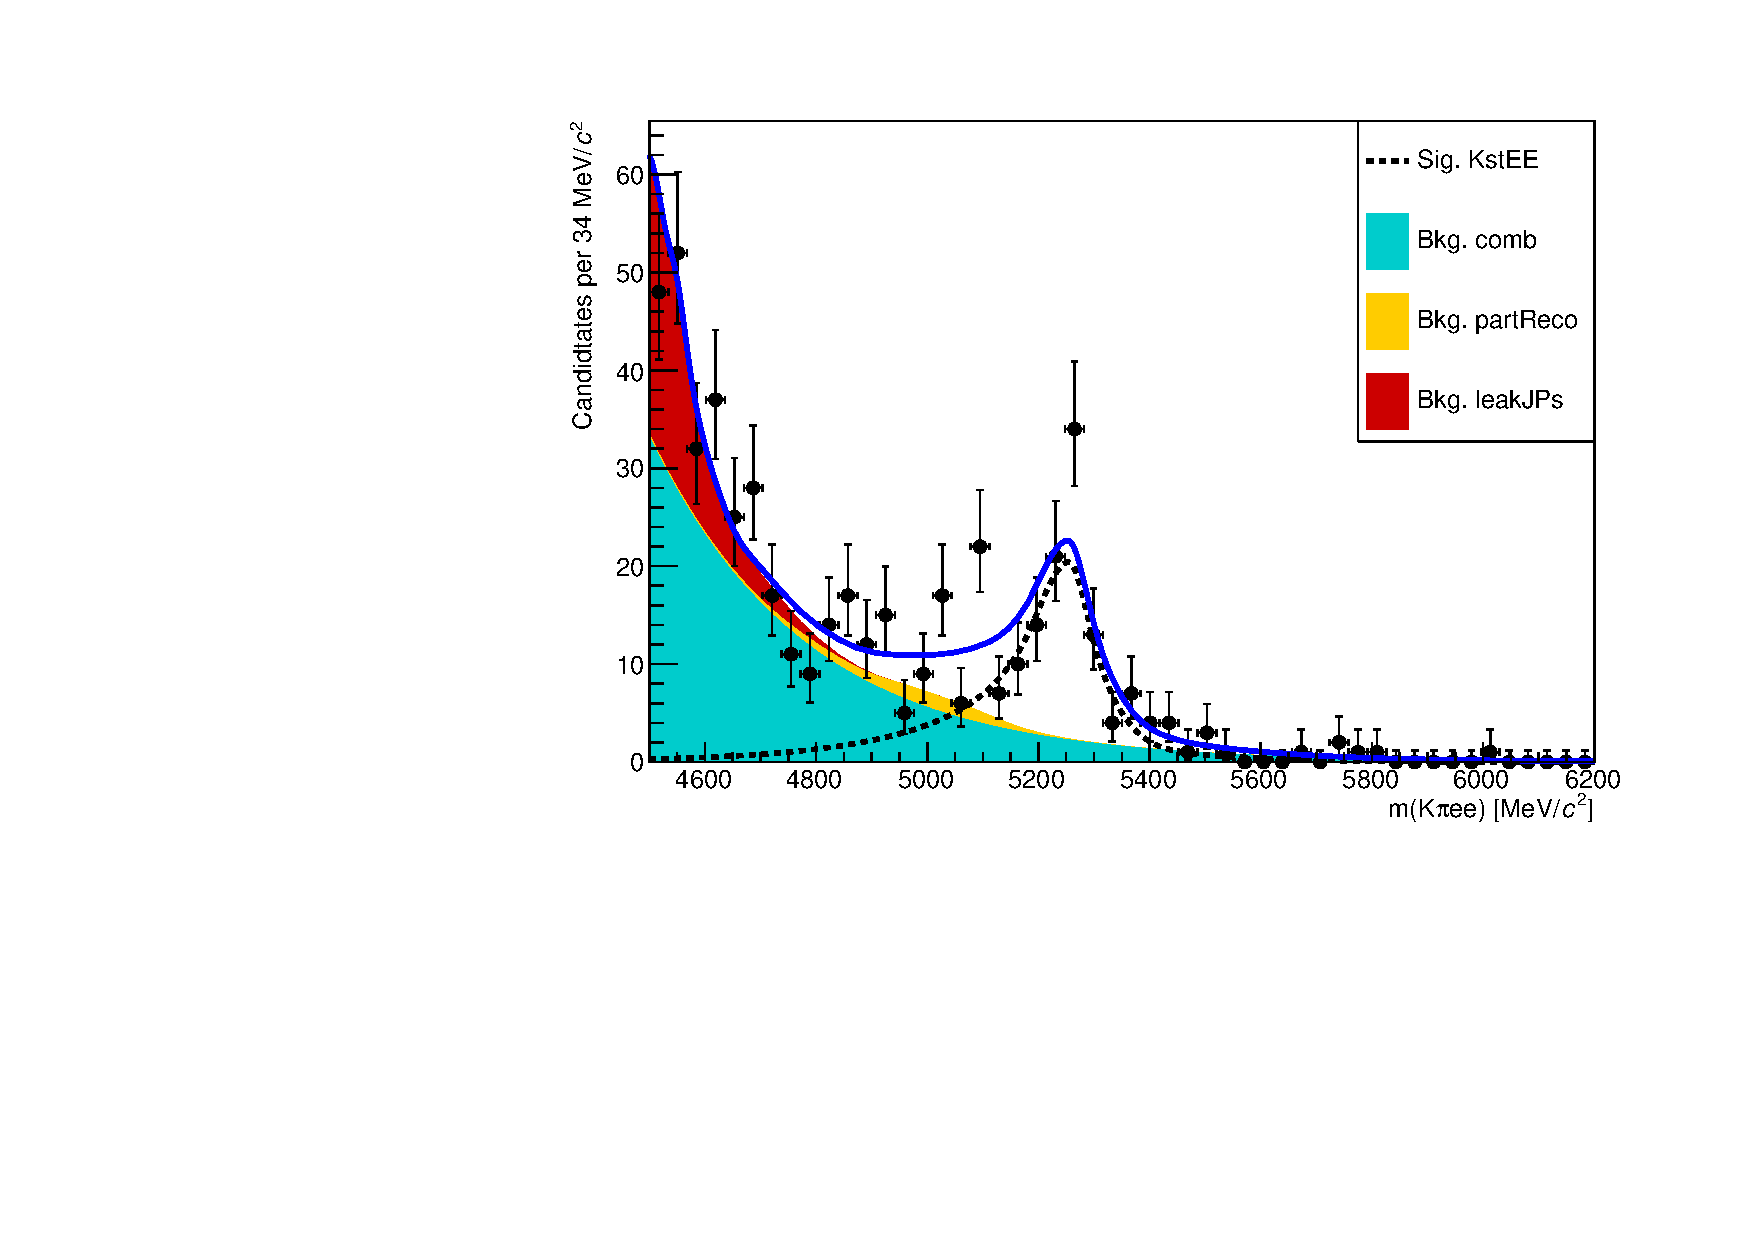
\includegraphics[width=0.7\textwidth]{RKst/figs/Fit/fit_EE/fit_EEc.pdf}
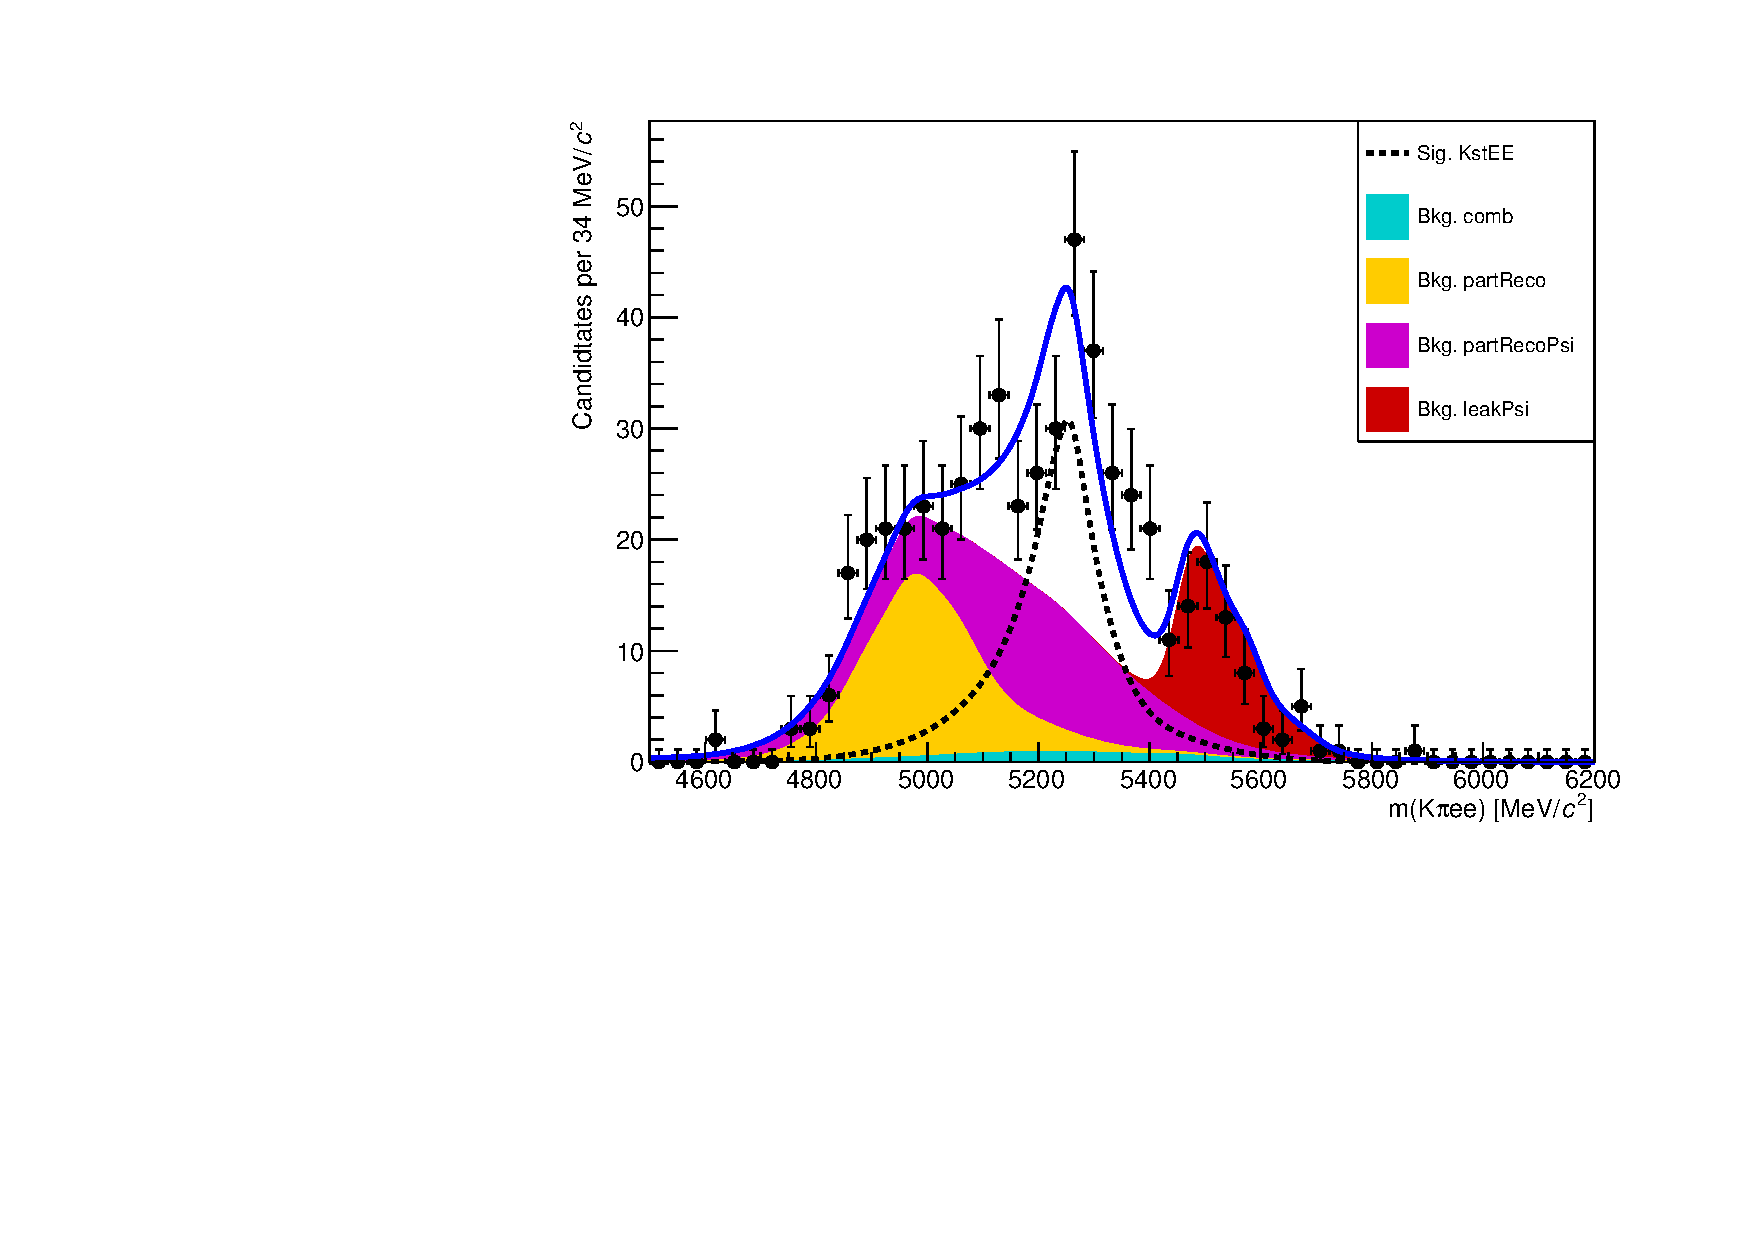
\includegraphics[width=0.7\textwidth]{RKst/figs/Fit/fit_EE/fit_EEh.pdf}
\caption{Fit to the \mKpiee invariant mass of \BdToKstee candidates. From top to bottom for the low-, central-
and high-\qsq intervals. The dashed black line represents the signal and the shaded shapes the backgrounds.}
\label{fig:fitsEE}
\end{figure}
%
\begin{figure}[h!]
\centering
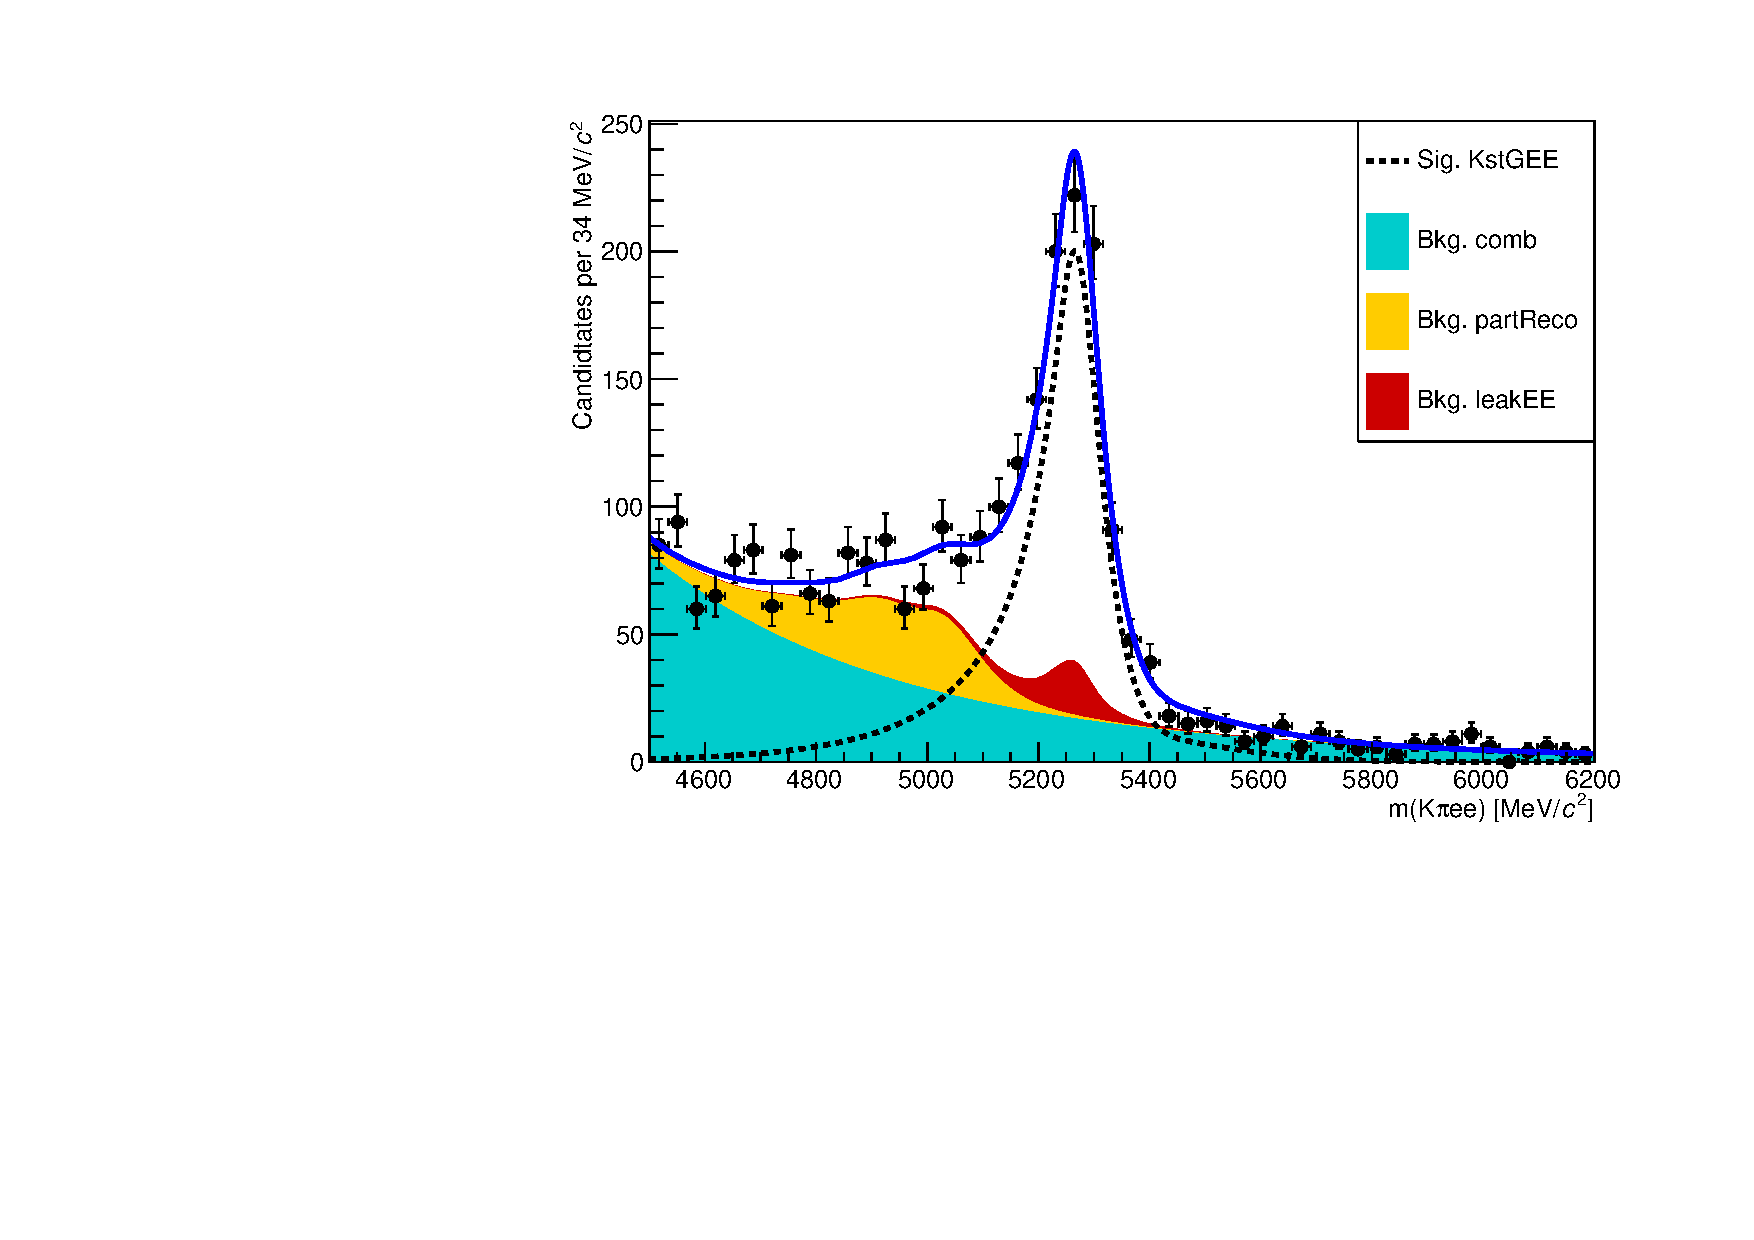
\includegraphics[width=0.7\textwidth]{RKst/figs/Fit/fit_EE/fit_G.pdf}
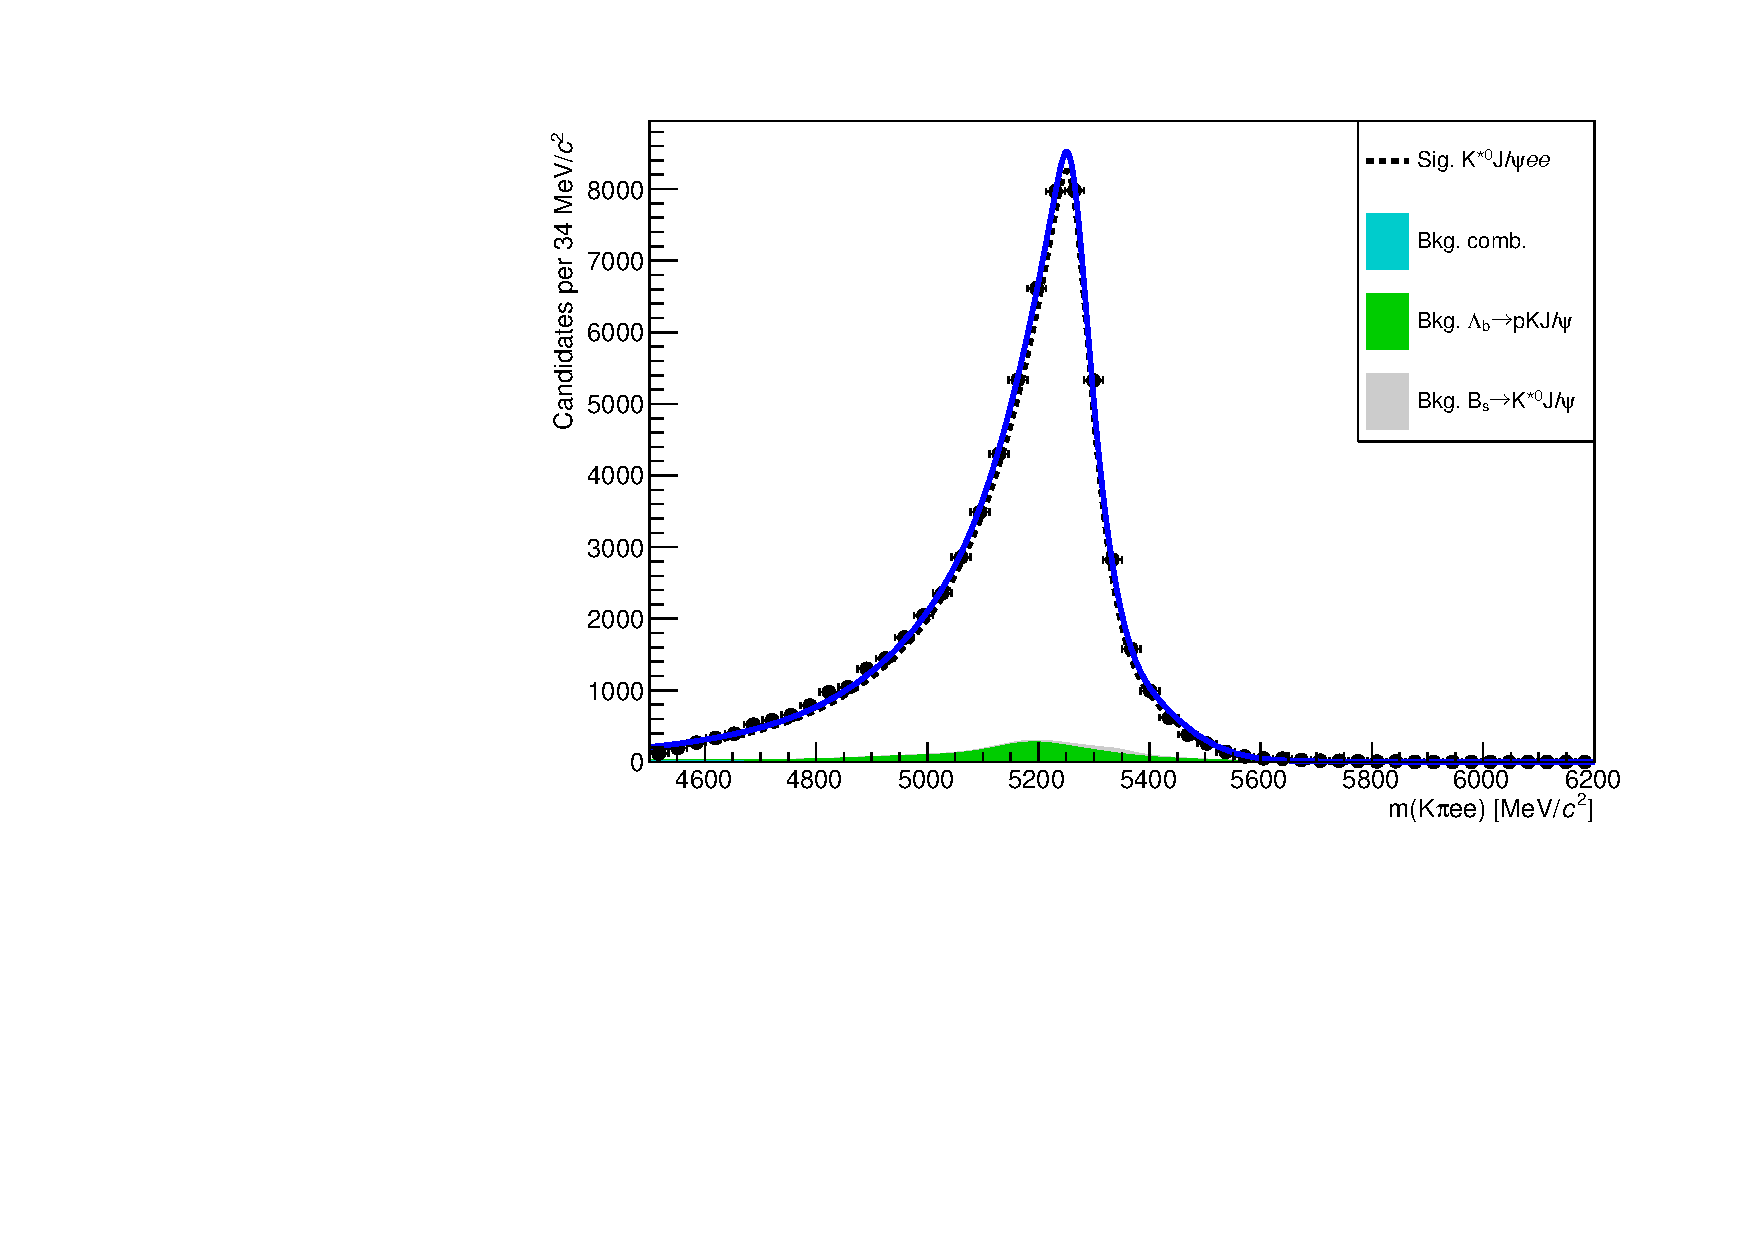
\includegraphics[width=0.7\textwidth]{RKst/figs/Fit/fit_EE/fit_JPs_P.pdf}
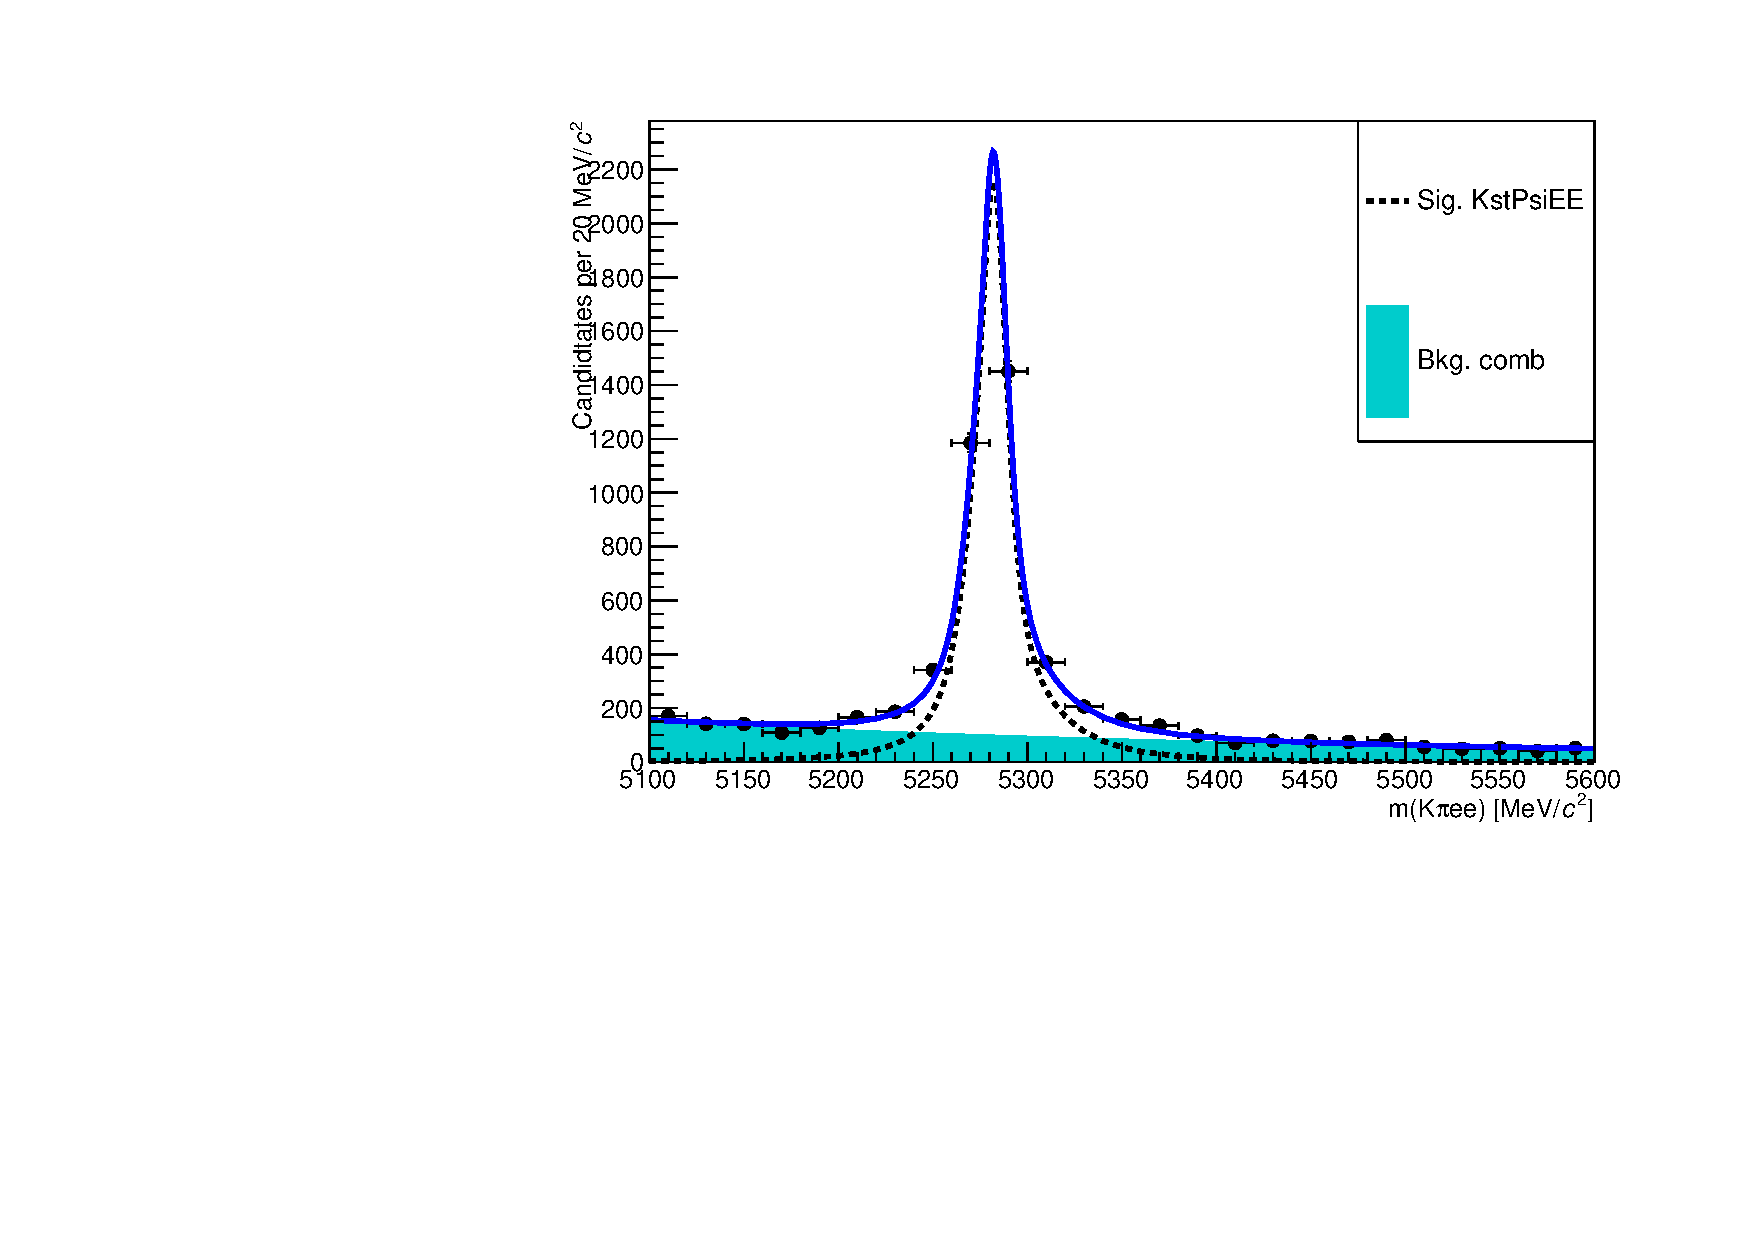
\includegraphics[width=0.7\textwidth]{RKst/figs/Fit/fit_EE/fit_Psi.pdf}
\caption{Fit to the \mKpiee invariant mass of control channel candidates.
From top to bottom: the invariant mass distribution without mass constraint of \BdToKstGee
and \BdToKstJPsee candidates and the constrained invariant mass, $\mKpiee_{\psi}$, of \BdToKstPsiee candidates.
The dashed black line represents the signal and the shaded shapes the backgrounds.}
\label{fig:fitsControlEE}
\end{figure}

\clearpage

